\documentclass[a4paper,11pt,twoside,openright]{report}
\usepackage[left=2cm,right=2cm,top=2cm,bottom=3cm]{geometry}
\usepackage{xspace}
\usepackage{listings}
\usepackage{color}
\usepackage[backref]{hyperref}
\usepackage[fleqn]{amsmath}
\usepackage{amsmath,amsfonts,amssymb,stmaryrd}
\usepackage{fancybox}
\usepackage{subfigure}
\usepackage{multirow}
\usepackage[table,xcdraw]{xcolor}
\usepackage[utf8]{inputenc}
\usepackage{graphicx}
\usepackage{verbatim}
\usepackage{latexsym}
\usepackage{mathchars}
\usepackage{setspace}
\usepackage{color}

\setlength{\parskip}{\medskipamount}  % a little space before a \par
\setlength{\parindent}{0pt}	      % don't indent first lines of paragraphs
%UHEAD.STY  If this is included after \documentstyle{report}, it adds
% an underlined heading style to the LaTeX report style.
% \pagestyle{uheadings} will put underlined headings at the top
% of each page. The right page headings are the Chapter titles and
% the left page titles are supplied by \def\lefthead{text}.

% Ted Shapin, Dec. 17, 1986

\makeatletter
\def\chapapp2{Chapter}

\def\appendix{\par
 \setcounter{chapter}{0}
 \setcounter{section}{0}
 \def\chapapp2{Appendix}
 \def\@chapapp{Appendix}
 \def\thechapter{\Alph{chapter}}}

\def\ps@uheadings{\let\@mkboth\markboth
% modifications
\def\@oddhead{\protect\underline{\protect\makebox[\textwidth][l]
		{\sl\rightmark\hfill\rm\thepage}}}
\def\@oddfoot{}
\def\@evenfoot{}
\def\@evenhead{\protect\underline{\protect\makebox[\textwidth][l]
		{\rm\thepage\hfill\sl\leftmark}}}
% end of modifications
\def\chaptermark##1{\markboth {\ifnum \c@secnumdepth >\m@ne
 \chapapp2\ \thechapter. \ \fi ##1}{}}%
\def\sectionmark##1{\markright {\ifnum \c@secnumdepth >\z@
   \thesection. \ \fi ##1}}}
\makeatother
%%From: marcel@cs.caltech.edu (Marcel van der Goot)
%%Newsgroups: comp.text.tex
%%Subject: illegal modification of boxit.sty
%%Date: 28 Feb 92 01:10:02 GMT
%%Organization: California Institute of Technology (CS dept)
%%Nntp-Posting-Host: andromeda.cs.caltech.edu
%%
%%
%%Quite some time ago I posted a file boxit.sty; maybe it made it
%%to some archives, although I don't recall submitting it. It defines
%%	\begin{boxit}
%%	...
%%	\end{boxit}
%%to draw a box around `...', where the `...' can contain other
%%environments (e.g., a verbatim environment). Unfortunately, it had
%%a problem: it did not work if you used it in paragraph mode, i.e., it
%%only worked if there was an empty line in front of \begin{boxit}.
%%Luckily, that is easily corrected.
%%
%%HOWEVER, apparently someone noticed the problem, tried to correct it,
%%and then distributed this modified version. That would be fine with me,
%%except that:
%%1. There was no note in the file about this modification, it only has my
%%   name in it.
%%2. The modification is wrong: now it only works if there is *no* empty
%%   line in front of \begin{boxit}. In my opinion this bug is worse than
%%   the original one.
%%
%%In particular, the author of this modification tried to force an empty
%%line by inserting a `\\' in the definition of \Beginboxit. If you have
%%a version of boxit.sty with a `\\', please delete it. If you have my
%%old version of boxit.sty, please also delete it. Below is an improved
%%version.
%%
%%Thanks to Joe Armstrong for drawing my attention to the bug and to the
%%illegal version.
%%
%%                                          Marcel van der Goot
%% .---------------------------------------------------------------
%% | Blauw de viooltjes,                    marcel@cs.caltech.edu
%% |    Rood zijn de rozen;
%% | Een rijm kan gezet
%% |    Met plaksel en dozen.
%% |


% boxit.sty
% version: 27 Feb 1992
%
% Defines a boxit environment, which draws lines around its contents.
% Usage:
%   \begin{boxit}
%	... (text you want to be boxed, can contain other environments)
%   \end{boxit}
%
% The width of the box is the width of the contents.
% The boxit* environment behaves the same, except that the box will be
% at least as wide as a normal paragraph.
%
% The reason for writing it this way (rather than with the \boxit#1 macro
% from the TeXbook), is that now you can box verbatim text, as in
%   \begin{boxit}
%   \begin{verbatim}
%   this better come out in boxed verbatim mode ...
%   \end{verbatim}
%   \end{boxit}
%
%						Marcel van der Goot
%						marcel@cs.caltech.edu
%

\def\Beginboxit
   {\par
    \vbox\bgroup
	   \hrule
	   \hbox\bgroup
		  \vrule \kern1.2pt %
		  \vbox\bgroup\kern1.2pt
   }

\def\Endboxit{%
			      \kern1.2pt
		       \egroup
		  \kern1.2pt\vrule
		\egroup
	   \hrule
	 \egroup
   }	

\newenvironment{boxit}{\Beginboxit}{\Endboxit}
\newenvironment{boxit*}{\Beginboxit\hbox to\hsize{}}{\Endboxit}
\pagestyle{empty}

\setlength{\parskip}{2ex plus 0.5ex minus 0.2ex}
\setlength{\parindent}{0pt}

\makeatletter  %to avoid error messages generated by "\@". Makes Latex treat "@" like a letter

\linespread{1.5}
\def\submitdate#1{\gdef\@submitdate{#1}}

\def\maketitle{
  \begin{titlepage}{
    %\linespread{1.5}
    \Large Universit\'e Nice-Sophia Antipolis \\
    %\linebreak
    \'ECOLE DOCTORALE STIC \\
	SCIENCES ET TECHNOLOGIES DE L’INFORMATION ET DE LA COMMUNICATION\\
    %\linebreak
    %Department of Computing
    \rm
    \vskip 3in
    \Large \bf \@title \par
  }
  \vskip 0.3in
  \par
  {\Large \@author}
  \vskip 4in
  \par
  Submitted in part fulfilment of the requirements for the degree of 
  \linebreak
  Doctor of Philosophy in Computing of the Universit\'e Nice-Sophia Antipolis
  \linebreak
  %the Diploma of Imperial College, \@submitdate
  \vfil
  \end{titlepage}
}

\def\titlepage{
  \newpage
  \centering
  \linespread{1}
  \normalsize
  \vbox to \vsize\bgroup\vbox to 9in\bgroup
}
\def\endtitlepage{
  \par
  \kern 0pt
  \egroup
  \vss
  \egroup
  \cleardoublepage
}

\def\abstract{
  \begin{center}{
    \large\bf Abstract}
  \end{center}
  \small
  %\def\baselinestretch{1.5}
  \linespread{1.5}
  \normalsize
}
\def\endabstract{
  \par
}

\newenvironment{acknowledgements}{
  \cleardoublepage
  \begin{center}{
    \large \bf Acknowledgements}
  \end{center}
  \small
  \linespread{1.5}
  \normalsize
}{\cleardoublepage}
\def\endacknowledgements{
  \par
}

\newenvironment{dedication}{
  \cleardoublepage
  \begin{center}{
    \large \bf Dedication}
  \end{center}
  \small
  \linespread{1.5}
  \normalsize
}{\cleardoublepage}
\def\enddedication{
  \par
}

\def\preface{
    \pagenumbering{roman}
    \pagestyle{plain}
    \doublespacing
}

\def\body{
    \cleardoublepage    
    \pagestyle{uheadings}
    \tableofcontents
    \pagestyle{plain}
    \cleardoublepage
    \pagestyle{uheadings}
    \listoftables
    \pagestyle{plain}
    \cleardoublepage
    \pagestyle{uheadings}
    \listoffigures
    \pagestyle{plain}
    \cleardoublepage
    \pagestyle{uheadings}
    \pagenumbering{arabic}
    \doublespacing
}

\makeatother  %to avoid error messages generated by "\@". Makes Latex treat "@" like a letter

\newcommand{\ipc}{{\sf ipc}}

\newcommand{\Prob}{\bbbp}
\newcommand{\Real}{\bbbr}
\newcommand{\real}{\Real}
\newcommand{\Int}{\bbbz}
\newcommand{\Nat}{\bbbn}

\newcommand{\NN}{{\sf I\kern-0.14emN}}   % Natural numbers
\newcommand{\ZZ}{{\sf Z\kern-0.45emZ}}   % Integers
\newcommand{\QQQ}{{\sf C\kern-0.48emQ}}   % Rational numbers
\newcommand{\RR}{{\sf I\kern-0.14emR}}   % Real numbers
\newcommand{\KK}{{\cal K}}
\newcommand{\OO}{{\cal O}}
\newcommand{\AAA}{{\bf A}}
\newcommand{\HH}{{\bf H}}
\newcommand{\II}{{\bf I}}
\newcommand{\LL}{{\bf L}}
\newcommand{\PP}{{\bf P}}
\newcommand{\PPprime}{{\bf P'}}
\newcommand{\QQ}{{\bf Q}}
\newcommand{\UU}{{\bf U}}
\newcommand{\UUprime}{{\bf U'}}
\newcommand{\zzero}{{\bf 0}}
\newcommand{\ppi}{\mbox{\boldmath $\pi$}}
\newcommand{\aalph}{\mbox{\boldmath $\alpha$}}
\newcommand{\bb}{{\bf b}}
\newcommand{\ee}{{\bf e}}
\newcommand{\mmu}{\mbox{\boldmath $\mu$}}
\newcommand{\vv}{{\bf v}}
\newcommand{\xx}{{\bf x}}
\newcommand{\yy}{{\bf y}}
\newcommand{\zz}{{\bf z}}
\newcommand{\oomeg}{\mbox{\boldmath $\omega$}}
\newcommand{\res}{{\bf res}}
\newcommand{\cchi}{{\mbox{\raisebox{.4ex}{$\chi$}}}}
%\newcommand{\cchi}{{\cal X}}
%\newcommand{\cchi}{\mbox{\Large $\chi$}}

% Logical operators and symbols
\newcommand{\imply}{\Rightarrow}
\newcommand{\bimply}{\Leftrightarrow}
\newcommand{\union}{\cup}
\newcommand{\intersect}{\cap}
\newcommand{\boolor}{\vee}
\newcommand{\booland}{\wedge}
\newcommand{\boolimply}{\imply}
\newcommand{\boolbimply}{\bimply}
\newcommand{\boolnot}{\neg}
\newcommand{\boolsat}{\!\models}
\newcommand{\boolnsat}{\!\not\models}

\renewcommand*{\lstlistlistingname}{List of Listings}
\newcommand{\op}[1]{\mathrm{#1}}
\newcommand{\s}[1]{\ensuremath{\mathcal #1}}

% Properly styled differentiation and integration operators
\newcommand{\diff}[1]{\mathrm{\frac{d}{d\mathit{#1}}}}
\newcommand{\diffII}[1]{\mathrm{\frac{d^2}{d\mathit{#1}^2}}}
\newcommand{\intg}[4]{\int_{#3}^{#4} #1 \, \mathrm{d}#2}
\newcommand{\intgd}[4]{\int\!\!\!\!\int_{#4} #1 \, \mathrm{d}#2 \, \mathrm{d}#3}

% Large () brackets on different lines of an eqnarray environment
\newcommand{\Leftbrace}[1]{\left(\raisebox{0mm}[#1][#1]{}\right.}
\newcommand{\Rightbrace}[1]{\left.\raisebox{0mm}[#1][#1]{}\right)}

% Funky symobols for footnotes
\newcommand{\symbolfootnote}{\renewcommand{\thefootnote}{\fnsymbol{footnote}}}
% now add \symbolfootnote to the beginning of the document...

\newcommand{\normallinespacing}{\renewcommand{\baselinestretch}{1.5} \normalsize}
\newcommand{\mediumlinespacing}{\renewcommand{\baselinestretch}{1.2} \normalsize}
\newcommand{\narrowlinespacing}{\renewcommand{\baselinestretch}{1.0} \normalsize}
\newcommand{\bump}{\noalign{\vspace*{\doublerulesep}}}
\newcommand{\cell}{\multicolumn{1}{}{}}
\newcommand{\spann}{\mbox{span}}
\newcommand{\diagg}{\mbox{diag}}
\newcommand{\modd}{\mbox{mod}}
\newcommand{\minn}{\mbox{min}}
\newcommand{\andd}{\mbox{and}}
\newcommand{\forr}{\mbox{for}}
\newcommand{\EE}{\mbox{E}}

\newcommand{\deff}{\stackrel{\mathrm{def}}{=}}
\newcommand{\syncc}{~\stackrel{\textstyle \rhd\kern-0.57em\lhd}{\scriptstyle L}~}

\def\coop{\mbox{\large $\rhd\!\!\!\lhd$}}
\newcommand{\sync}[1]{\raisebox{-1.0ex}{$\;\stackrel{\coop}{\scriptscriptstyle
#1}\,$}}

\newtheorem{definition}{Definition}[chapter]
\newtheorem{theorem}{Theorem}[chapter]

\newcommand{\Figref}[1]{Figure~\ref{#1}}
\newcommand{\fig}[3]{
 \begin{figure}[!ht]
 \begin{center}
 \scalebox{#3}{\includegraphics{figs/#1.ps}}
 \vspace{-0.1in}
 \caption[ ]{\label{#1} #2}
 \end{center}
 \end{figure}
}

\newcommand{\figtwo}[8]{
 \begin{figure}
 \parbox[b]{#4 \textwidth}{
 \begin{center}
 \scalebox{#3}{\includegraphics{figs/#1.ps}}
 \vspace{-0.1in}
 \caption{\label{#1}#2}
 \end{center}
 }
 \hfill
 \parbox[b]{#8 \textwidth}{
 \begin{center}
 \scalebox{#7}{\includegraphics{figs/#5.ps}}
 \vspace{-0.1in}
 \caption{\label{#5}#6}
 \end{center}
 }
 \end{figure}
}

 \usepackage{booktabs}
 \usepackage{multirow}
 \usepackage[table,xcdraw]{xcolor}
 
 \usepackage{afterpage}
 \usepackage{pdflscape}
 
 %\usepackage{setspace}
 
 \usepackage[compact]{titlesec}
 %\titlespacing{\section}{0pt}{*0}{*0}
 %\titlespacing{\subsection}{0pt}{*0}{*0}
 %\titlespacing{\subsubsection}{0pt}{*0}{*0}
 
 \usepackage{enumitem}
  % space in list and enumerate
 \setlist[itemize]{topsep=0ex}
 
 % space between lines in paragraphs
 %\singlespacing

 % eliminate space between paragraph
\setlength{\parskip}{1em}
 
 
 \newcommand*{\englishTitle}[1]{\def\engTitle{#1}}
 \newcommand*{\frenchTitle}[1]{\def\frTitle{#1}}
 \newcommand*{\director}[1]{\def\dirName{#1}}
 \newcommand*{\directorTitle}[1]{\def\dirTitle{#1}}
 \newcommand*{\directorAffiliation}[1]{\def\dirAff{#1}} 
 \newcommand*{\supervisor}[1]{\def\supName{#1}}
 \newcommand*{\supervisorTitle}[1]{\def\supTitle{#1}}
 \newcommand*{\supervisorAffiliation}[1]{\def\supAff{#1}} 
 \newcommand*{\reviewerOne}[1]{\def\revOneName{#1}}
 \newcommand*{\reviewerOneTitle}[1]{\def\revOneTitle{#1}}
 \newcommand*{\reviewerOneAffiliation}[1]{\def\revOneAff{#1}}
 \newcommand*{\reviewerTwo}[1]{\def\revTwoName{#1}}
 \newcommand*{\reviewerTwoTitle}[1]{\def\revTwoTitle{#1}}
 \newcommand*{\reviewerTwoAffiliation}[1]{\def\revTwoAff{#1}}
 \newcommand*{\president}[1]{\def\presName{#1}}
 \newcommand*{\presidentTitle}[1]{\def\presTitle{#1}} 
 \newcommand*{\presidentAffiliation}[1]{\def\presAff{#1}}
 \newcommand*{\examinerOne}[1]{\def\examOneName{#1}}
 \newcommand*{\examinerOneTitle}[1]{\def\examOneTitle{#1}}
 \newcommand*{\examinerOneAffiliation}[1]{\def\examOneAff{#1}}
 \newcommand*{\examinerTwo}[1]{\def\examTwoName{#1}}
 \newcommand*{\examinerTwoTitle}[1]{\def\examTwoTitle{#1}}
 \newcommand*{\examinerTwoAffiliation}[1]{\def\examTwoAff{#1}}
 \renewcommand*{\author}[1]{\def\authornames{#1}}
 \newcommand\maketitletesis{
 	\begin{titlepage}
 		\newgeometry{	
 			left=1.5in,	
 			top=0.5in,
 			right=.5in,	
 			bottom=1.2in,
 			headheight = 20.0pt,
 			headsep = 0.25in,
 			footskip = 0.3in
 		}
 		\begin{center}
 			\noindent {\large \textbf{UNIVERSIT\'E NICE - SOPHIA ANTIPOLIS}} \\
 			\vspace*{0.3cm}
 			\noindent {\LARGE \textbf{\'ECOLE DOCTORALE STIC}} \\
 			\noindent \textbf{SCIENCES ET TECHNOLOGIES DE L'INFORMATION \\ ET DE LA COMMUNICATION} \\
 			\vspace*{0.5cm}
 			\noindent \Huge \textbf{T H \`E S E} \\
 			\vspace*{0.3cm}
 			\noindent \large {pour l'obtention du grade de} \\
 			\vspace*{0.3cm}
 			\noindent \LARGE \textbf{Docteur en Sciences} \\
 			\vspace*{0.3cm}
 			\noindent \Large de l'Universit\'e Nice - Sophia Antipolis \\
 			\noindent \Large \textbf{Mention : \textsc{Informatique}}\\
 			\vspace*{0.4cm}
 			\noindent \large {present\'ee et soutenue par\\}
 			\noindent \authornames \\
 			\vspace*{0.5cm}
 			\noindent {\Huge \textbf{\frTitle}} \\
 			\vspace*{0.3cm}
 			\noindent {\Large \textbf{\engTitle}} \\
 			\vspace*{0.5cm}
 			\noindent \Large Th\`ese dirig\'ee par: \dirName \\
 			%\vspace*{10mm}
 			\noindent \Large et encadr\'ee par: \supName \\
 			%\noindent \Large pr\'epar\'ee \`a l'INRIA Sophia Antipolis, Projet \textsc{\groupname}\\
 			\vspace*{0.2cm}
 			\noindent \large soutenue le 27 F\'evrier 2016 \\
 			\vspace*{0.3cm}
 		\end{center}
 		\noindent \large \textbf{Jury :}
 		\begin{center}
 			%\noindent \large 
 			\begin{tabular}{llccl}
 				%	  M.		& \presName 		& \presTitle		&	\presAff		& \textit{Pr\'esident}\\
 				M.		& \revOneName 	& \revOneTitle	&	\revOneAff	& \textit{Rapporteur}\\
 				M.		& \revTwoName	& \revTwoTitle	&	\revTwoAff	& \textit{Rapporteur}\\	
 				M.		& \examOneName	& \examOneTitle	&	\examOneAff	& \textit{Examinateur}\\
 				M.		& \examTwoName	& \examTwoTitle 	&	\examTwoAff	& \textit{Examinateur}\\
 				M.		& \dirName 		& \dirTitle		&	\dirAff		& \textit{Directeur de Th\`ese}\\
 				M. 	& \supName 		& \supTitle		&	\supAff		& \textit{Encadrant}\\
 			\end{tabular}
 		\end{center}
 		\restoregeometry
 	\end{titlepage}
 }
 
 
 %\usepackage[acronym]{glossaries}
 %\makeglossaries
 %\include{glossaryDES}

\newcommand{\tsq}{\textsc{TimeSquare}\xspace}
\newcommand{\ccsl}{\textsc{ccsl}\xspace}
\newcommand{\ecl}{\textsc{ecl}\xspace}
\newcommand{\as}{\textsc{as}\xspace}
\newcommand{\dsa}{\textsc{dsa}\xspace}
\newcommand{\dse}{\textsc{dse}\xspace}
\newcommand{\mse}{\textsc{mse}\xspace}
\newcommand{\mocc}{\textsc{mocc}\xspace}
\newcommand{\moccml}{\textsc{moccml}\xspace}
\newcommand{\ie}{\emph{i.e.,~}}
\newcommand{\eg}{\emph{e.g.},~}
\newcommand{\bcool}{\textsc{B-COoL}\xspace}
\newcommand{\bflow}{\textsc{B-FloW}\xspace}
\newcommand{\todo}[1]{{\color{blue}\fcolorbox{red}{yellow}{\textbf{TODO:}} #1}}

\definecolor{KRed}{rgb}{0.59,0,0}
\definecolor{KBlue}{rgb}{0,0,0.59}
\definecolor{KBlack}{rgb}{0,0,0}
\definecolor{KGreen}{rgb}{0,0.59,0}
\definecolor{KPurple}{rgb}{0.5,0,0.47}
\definecolor{KOliveGreen}{cmyk}{0.64,0,0.95,0.40}

\definecolor{DBlue}{rgb}{0,0,0.4}
\definecolor{DRed}{rgb}{0.4,0,0}
\definecolor{CGreen}{rgb}{0.3,0.7,0.4}
\definecolor{OliveGreen}{rgb}{0.3,0.7,0.4}
\definecolor{LGrey}{rgb}{0.95,0.95,0.95}


\lstdefinelanguage{ecl}
{
	morekeywords=[0]{ require, using, extern, pre, post, inv},
	morekeywords=[1]{activitydiagram, tfsm},
	morekeywords=[2]{ aspect, abstract },
	morekeywords=[3]{ end, Operator, operator },
	morekeywords=[4]{ package, context, def, Event, self},
	morekeywords=[5]{  },
	morekeywords=[6]{ and, or, not },
	sensitive=true,
	morecomment=[l]{//},
	morecomment=[s]{/*}{*/},
	morestring=[b]",
}

\lstset{language=ecl,
	basicstyle=\ttfamily,
	keywordstyle=[0]\bf\color{KRed},
	keywordstyle=[1]\bf\color{KBlue},
	keywordstyle=[2]\textit\bf\color{KBlue},
	keywordstyle=[3]\bf\color{KBlue},
	keywordstyle=[4]\textit\bf\color{KPurple},
	keywordstyle=[5]\bf\color{KBlack},
	keywordstyle=[6]\bf\color{KPurple},
	commentstyle=\color{KOliveGreen},
	tabsize=2,
	breaklines=true,
	aboveskip=1pt,
	belowskip=1pt,
	numbersep=3pt
	%   frame=single,
	%   backgroundcolor=\color{Gris}    
}

\lstdefinelanguage{bcool}
{
	morekeywords=[0]{ require, using, extern, pre, post, inv},
	morekeywords=[1]{activity, tfsm},
	morekeywords=[2]{},
	morekeywords=[3]{ end, Operator, operator, BCOoLSpec},
	morekeywords=[4]{ ImportLib, ImportInterface, as, when, do, CorrespondenceMatching, Event, Local, Global},
	morekeywords=[5]{ occurs, startAction, finishAction, entering, leaving, startActivity, finishActivity, ticks, firing},
	morekeywords=[6]{ and, or, not },
	sensitive=true,
	morecomment=[l]{//},
	morecomment=[s]{/*}{*/},
	morestring=[b]",
}

\lstset{language=bcool,
	basicstyle=\ttfamily,
	keywordstyle=[0]\bf\color{KRed},
	keywordstyle=[1]\bf\color{KBlue},
	keywordstyle=[2]\textit\bf\color{KBlue},
	keywordstyle=[3]\bf\color{KBlue},
	keywordstyle=[4]\textit\bf\color{KPurple},
	keywordstyle=[5]\bf\color{KBlack},
	keywordstyle=[6]\bf\color{KPurple},
	commentstyle=\color{KOliveGreen},
	tabsize=2,
	breaklines=true,
	aboveskip=5pt,
	belowskip=5pt,
	numbersep=3pt
	%   frame=single,
	%   backgroundcolor=\color{Gris}    
}

\lstdefinelanguage{moccml}
{
	morekeywords=[0]{ require, using, extern, pre, post, inv},
	morekeywords=[1]{dse, Coincides, Causes, SampleBy, root, integer},
	morekeywords=[2]{"./ccsllibrary/kernel.ccslLib","./ccsllibrary/CCSL.ccslLib"},
	morekeywords=[3]{ end, Operator, operator, BCOoLSpec},
	morekeywords=[4]{ ClockConstraintSystem, Block, entryBlock, RelationDefinition, Relation, AutomataConstraintLibrary, RelationDeclarations, as, RelationLibrary, ExpressionLibrary, RelationDefinitions, RelationDeclaration, imports, BCoolLibrary, import, ExpressionDeclarations, ExpressionDefinitions, ExpressionDefinition, ExpressionDeclaration},
	morekeywords=[5]{ occurs, startAction, finishAction, entering, leaving, startActivity, finishActivity, ticks},
	morekeywords=[6]{ and, or, not },
	sensitive=true,
	morecomment=[l]{//},
	morecomment=[s]{/*}{*/},
	morestring=[b]",
}

\lstset{language=moccml,
	basicstyle=\ttfamily,
	keywordstyle=[0]\bf\color{KRed},
	keywordstyle=[1]\bf\color{KBlue},
	keywordstyle=[2]\textit\bf\color{KBlue},
	keywordstyle=[3]\bf\color{KBlue},
	keywordstyle=[4]\textit\bf\color{KPurple},
	keywordstyle=[5]\bf\color{KBlack},
	keywordstyle=[6]\bf\color{KPurple},
	commentstyle=\color{KOliveGreen},
	tabsize=2,
	breaklines=true,
	%   frame=single,
	%   backgroundcolor=\color{Gris}    
}


\lstdefinelanguage{bflow}
{
	morekeywords=[0]{ require, using, extern, pre, post, inv},
	morekeywords=[1]{activity, tfsm},
	morekeywords=[2]{},
	morekeywords=[3]{ end, Operator, operator, BCOoLFlow, Flow},
	morekeywords=[4]{ ImportBCOoL, ImportInterface, as, when, do, Model, applies, between, CorrespondenceMatching, Event, Local, Global},
	morekeywords=[5]{ occurs, startAction, finishAction, entering, leaving, startActivity, finishActivity, ticks, firing},
	morekeywords=[6]{ and, or, not },
	sensitive=true,
	morecomment=[l]{//},
	morecomment=[s]{/*}{*/},
	morestring=[b]",
}

\lstset{language=bflow,
	basicstyle=\ttfamily,
	keywordstyle=[0]\bf\color{KRed},
	keywordstyle=[1]\bf\color{KBlue},
	keywordstyle=[2]\textit\bf\color{KBlue},
	keywordstyle=[3]\bf\color{KBlue},
	keywordstyle=[4]\textit\bf\color{KPurple},
	keywordstyle=[5]\bf\color{KBlack},
	keywordstyle=[6]\bf\color{KPurple},
	commentstyle=\color{KOliveGreen},
	tabsize=2,
	breaklines=true,
	aboveskip=5pt,
	belowskip=5pt,
	numbersep=3pt
	%   frame=single,
	%   backgroundcolor=\color{Gris}    
}


\lstdefinelanguage{epsilon}
{
	morekeywords=[0]{ require, using, extern, pre, post, inv},
	morekeywords=[1]{activity, tfsm},
	morekeywords=[2]{},
	morekeywords=[3]{ end, Operator, operator, BCOoLFlow, Flow},
	morekeywords=[4]{ ImportBCOoL, ImportInterface, as, when, do, Model, applies, between, CorrespondenceMatching, Event, Local, Global, rule, match, with, compare, return},
	morekeywords=[5]{ occurs, startAction, finishAction, entering, leaving, startActivity, finishActivity, ticks, firing},
	morekeywords=[6]{ and, or, not },
	sensitive=true,
	morecomment=[l]{//},
	morecomment=[s]{/*}{*/},
	morestring=[b]",
}

\lstset{language=epsilon,
	basicstyle=\ttfamily,
	keywordstyle=[0]\bf\color{KRed},
	keywordstyle=[1]\bf\color{KBlue},
	keywordstyle=[2]\textit\bf\color{KBlue},
	keywordstyle=[3]\bf\color{KBlue},
	keywordstyle=[4]\textit\bf\color{KPurple},
	keywordstyle=[5]\bf\color{KBlack},
	keywordstyle=[6]\bf\color{KPurple},
	commentstyle=\color{KOliveGreen},
	tabsize=2,
	breaklines=true,
	aboveskip=5pt,
	belowskip=5pt,
	numbersep=3pt
	%   frame=single,
	%   backgroundcolor=\color{Gris}    
}


\newcommand*{\englishTitle}[1]{\def\engTitle{#1}}
\newcommand*{\frenchTitle}[1]{\def\frTitle{#1}}
\newcommand*{\director}[1]{\def\dirName{#1}}
\newcommand*{\directorTitle}[1]{\def\dirTitle{#1}}
\newcommand*{\directorAffiliation}[1]{\def\dirAff{#1}} 
\newcommand*{\supervisor}[1]{\def\supName{#1}}
\newcommand*{\supervisorTitle}[1]{\def\supTitle{#1}}
\newcommand*{\supervisorAffiliation}[1]{\def\supAff{#1}} 
\newcommand*{\reviewerOne}[1]{\def\revOneName{#1}}
\newcommand*{\reviewerOneTitle}[1]{\def\revOneTitle{#1}}
\newcommand*{\reviewerOneAffiliation}[1]{\def\revOneAff{#1}}
\newcommand*{\reviewerTwo}[1]{\def\revTwoName{#1}}
\newcommand*{\reviewerTwoTitle}[1]{\def\revTwoTitle{#1}}
\newcommand*{\reviewerTwoAffiliation}[1]{\def\revTwoAff{#1}}
\newcommand*{\president}[1]{\def\presName{#1}}
\newcommand*{\presidentTitle}[1]{\def\presTitle{#1}} 
\newcommand*{\presidentAffiliation}[1]{\def\presAff{#1}}
\newcommand*{\examinerOne}[1]{\def\examOneName{#1}}
\newcommand*{\examinerOneTitle}[1]{\def\examOneTitle{#1}}
\newcommand*{\examinerOneAffiliation}[1]{\def\examOneAff{#1}}
\newcommand*{\examinerTwo}[1]{\def\examTwoName{#1}}
\newcommand*{\examinerTwoTitle}[1]{\def\examTwoTitle{#1}}
\newcommand*{\examinerTwoAffiliation}[1]{\def\examTwoAff{#1}}
\renewcommand*{\author}[1]{\def\authornames{#1}}
\newcommand\maketitletesis{
\begin{titlepage}
	\newgeometry{	
		left=1.5in,	
		top=0.5in,
		right=.5in,	
		bottom=1.2in,
		headheight = 20.0pt,
		headsep = 0.25in,
		footskip = 0.3in
	}
	\begin{center}
		\noindent {\large \textbf{UNIVERSIT\'E NICE - SOPHIA ANTIPOLIS}} \\
		\vspace*{0.3cm}
		\noindent {\LARGE \textbf{\'ECOLE DOCTORALE STIC}} \\
		\noindent \textbf{SCIENCES ET TECHNOLOGIES DE L'INFORMATION \\ ET DE LA COMMUNICATION} \\
		\vspace*{0.5cm}
		\noindent \Huge \textbf{T H \`E S E} \\
		\vspace*{0.3cm}
		\noindent \large {pour l'obtention du grade de} \\
		\vspace*{0.3cm}
		\noindent \LARGE \textbf{Docteur en Sciences} \\
		\vspace*{0.3cm}
		\noindent \Large de l'Universit\'e Nice - Sophia Antipolis \\
		\noindent \Large \textbf{Mention : \textsc{Informatique}}\\
		\vspace*{0.4cm}
		\noindent \large {present\'ee et soutenue par\\}
		\noindent \authornames \\
		\vspace*{0.5cm}
		\noindent {\Huge \textbf{\frTitle}} \\
		\vspace*{0.3cm}
		\noindent {\Large \textbf{\engTitle}} \\
		\vspace*{0.5cm}
		\noindent \Large Th\`ese dirig\'ee par: \dirName \\
		%\vspace*{10mm}
		\noindent \Large et encadr\'ee par: \supName \\
		%\noindent \Large pr\'epar\'ee \`a l'INRIA Sophia Antipolis, Projet \textsc{\groupname}\\
		\vspace*{0.2cm}
		\noindent \large soutenue le 27 F\'evrier 2016 \\
		\vspace*{0.3cm}
	\end{center}
	\noindent \large \textbf{Jury :}
	\begin{center}
		%\noindent \large 
		\begin{tabular}{llccl}
			%	  M.		& \presName 		& \presTitle		&	\presAff		& \textit{Pr\'esident}\\
			M.		& \revOneName 	& \revOneTitle	&	\revOneAff	& \textit{Rapporteur}\\
			M.		& \revTwoName	& \revTwoTitle	&	\revTwoAff	& \textit{Rapporteur}\\	
			M.		& \examOneName	& \examOneTitle	&	\examOneAff	& \textit{Examinateur}\\
			M.		& \examTwoName	& \examTwoTitle 	&	\examTwoAff	& \textit{Examinateur}\\
			M.		& \dirName 		& \dirTitle		&	\dirAff		& \textit{Directeur de Th\`ese}\\
			M. 	& \supName 		& \supTitle		&	\supAff		& \textit{Encadrant}\\
		\end{tabular}
	\end{center}
	\restoregeometry
\end{titlepage}
}


\begin{document}

\englishTitle{\bcool: A Language to Coordinate Concurrent Heterogeneous Systems}
\frenchTitle{\bcool: Un Language pour la Coordination de Syst\`emes Concurrents et H\'et\'erog\`enes}


\author{\LARGE Matias Ezequiel \textsc{Vara Larsen}}

\director{Fr\'ed\'eric \textsc{Mallet}}
\directorTitle{M.C.}
\directorAffiliation{INRIA/I3S-CNRS}
\reviewerOne{Olivier Barais}
\reviewerOneTitle{Prof.}
\reviewerOneAffiliation{Universit\'e de Rennes 1}
\reviewerTwo{Sebastien Gerard}
\reviewerTwoTitle{D.R.}
\reviewerTwoAffiliation{CEA LIST}
\examinerOne{??}
\examinerOneTitle{??}
\examinerOneAffiliation{??}
\examinerTwo{??}
\examinerTwoTitle{??}
\examinerTwoAffiliation{??}
\supervisor{Julien \textsc{DeAntoni}}
\supervisorTitle{M.C.}
\supervisorAffiliation{INRIA/I3S-CNRS}

\maketitletesis

\addcontentsline{toc}{chapter}{R\'esum\'e}

\begin{frenchabstract}
Les appareils modernes sont constitués de plusieurs sous-systèmes de différentes sortes qui communiquent et interagissent. L'hétérogénéité de ces sous-systèmes et leurs interactions complexes rendent très délicate leur développement. L'approche d'ingénierie dirigée par les modèles apporte une solution en permettant l'expression de nombreux modèles structurels et comportementaux de natures très diverses. Dans ce contexte, il est nécessaire de construire un modèle unique qui intègre ces différents modèles afin d'y appliquer des méthodes de validation et de vérification pour permettre aux ingénieurs système de comprendre et de valider un comportement global. Cependant, la coordination manuelle des différents modèles qui composent le système est une opération source d'erreurs et les approches automatiques proposent des patrons de coordination ad-hoc pour certaines paires de langages. Dans ces approches, le patron de coordination est souvent encapsulé dans un outil dont il est difficile d'extraire les liens avec le système global. Cette thèse propose le Behavioral Coordination Operator Language (\bcool), un langage dédié à la spécification de patrons de coordination entre des langages à partir de la définition d'opérateurs de coordination. Ces opérateurs sont employés afin d'automatiser la coordination de modèles exprimés dans ces langages. \bcool est implémenté comme une suite de plugins qui s'appuient sur l'Eclipse Modeling Framework et présente ainsi un environnement complet pour l'exécution et la vérification de différents modèles coordonnés. Nous illustrons cette approche avec la définition d'opérateurs de coordination entre deux langages: \emph{timed finite state machines} et  \emph{activities}. Ensuite, nous utilisons ces opérateurs afin de coordonner et d'exécuter un modèle hétérogène de caméra de surveillance.
\end{frenchabstract}



\cleardoublepage
\addcontentsline{toc}{chapter}{Abstract}


\begin{abstract}
Modern devices embed several subsystems with different characteristics that communicate and interact in many ways. This makes its development complex since a designer has to deal with the heterogeneity of each subsystem but also with the interactions among them. To tackle the development of complex systems, Model Driven Engineering promotes the use of various, possibly heterogeneous, structural and behavioral models. In this context, the coordination of behavioral models to produce a single integrated model is necessary to provide support for validation and verification. It allows system designers to understand and validate the global and emerging behavior of the system. However, the manual coordination of models is tedious and error-prone, and current approaches to automate the coordination are bound to a fixed set of coordination patterns. Moreover, automatic approaches encode the pattern into a tool thus limiting the reasoning on the global system behavior. In this thesis, we propose the Behavioral Coordination Operator Language (\bcool) to reify coordination patterns between specific domains by using coordination operators between the Domain-Specific Modeling Languages used in these domains. Those operators are then used to automate the coordination of models conforming to these languages. \bcool is implemented as plugins for the Eclipse Modeling Framework thus providing a complete environment to execute and verify coordinated models. We illustrate the use of \bcool with the definition of coordination operators between two languages: timed finite state machines and activities. We then use these operators to coordinate and execute the heterogeneous model of a surveillance camera system.
\end{abstract}
\cleardoublepage

\addcontentsline{toc}{chapter}{Acknowledgements}

\begin{acknowledgements}
%This thesis involved the collaboration of many people. My thanks go to:
%\begin{itemize}
%	\item My advisors Frederic Mallet and Julien DeAntoni whose advice improved my quality as research scientist.
%	\item The AOSTE team whose advice improved my research and for every launch that we got all together;
%	\item The GEMOC project for all the feedback during the PhD that helps me a lot for improving my results; 
%	\item The committee members, for serving as my committee members even at hardship. I also want to thank you for letting my defense be an enjoyable moment, and for your brilliant comments and suggestions, thanks to you;
%	\item My family Julio, Silvia, Pilar, Julian, and my grandparents la nona Dina, the Pichi and la abuela Maria. Without your support and encouragement, my success would not have been possible.   
%\end{itemize}



%I think I really grown as a research scientist. Your advice on research have been priceless. It has been a pleasure for me, to work in the AOSTE team during these years. I would like also to thanks 

%I would also like to thank my committee members, professor NAME SURNAME, professor NAME SURNAME, professor NAME SURNAME for serving as my committee members even at hardship. I also want to thank you for letting my defense be an enjoyable moment, and for your brilliant comments and suggestions, thanks to you.


%It has been a pleasure for me, to work in the AOSTE team during these years. I would like to address my special thanks to Charles André, who read and commented my first manuscript version, I miss his questions on Spanish grammar, always difficult to answer. My gratitude to Robert de Simone for welcoming me in the team, and also integrating me to the ANR-HELP project, which was in part an inspiration for this thesis; to Marie-Agnès Peraldi.


\end{acknowledgements}
\cleardoublepage

\begin{dedication}
  Dedication here.
\end{dedication}
\clearpage

\narrowlinespacing

\vspace*{4mm}
\emph{`For a true writer each book should be a new beginning where he tries again for something that is beyond attainment. He should always try for something that has never been done or that others have tried and failed. Then sometimes, with great luck, he will succeed.'}\\
\\

\normallinespacing

\hfill \hfill Ernest Hemingway

\body

\chapter{Introduction}

%\section{Context}

\begin{itemize}
	% context 
	% complex systems
	\item Nowadays devices are becoming more complex. They embed several subsystems with different characteristics that communicate and interact in many ways. For example, current cars can integrate an adaptive control cruise system, GPS tracking, fuel control system and soon on. Furthermore, these subsystems are widely coupled. For instance, the adaptive cruise system controls the way to get home depending on the GPS tacking, also, the fuel control system regulates the speed of the car depending on the level of fuel.
	
	% designing of complex systems
	\item This makes the designing of these systems very complex. A designer has to dealt with the heterogeneity of each subsystem but also with the interaction between them. To reduce the complexity of such a development, the designing is split into different domains, \eg mechanical, electronic, software. Therefore, the development of such complex system is talcked by different domains experts.
	
	% Multiple DSMLs --> heterogenenous
	\item In this context, Model Driven Engineering (MDE) has addressed the problem of the development of application for complex systems by proposing Domain Specific Modeling Languages (DSMLs). Each domain expert relies on a DSMLs to better describe its domain. Each DSMLs has its own expressiveness and properties. As a result of such development, several models conforming to different DSMLs are developed and the specification of the overall system becomes \emph{heterogeneous}.
% problem
	\item However, at some point of development, these models have to be integrated to understand the system and its emerging behavior globally. It is necessary to specify how models and languages are related to each other, in both a structural and a behavioral way. Whereas the MDE community provides some extensive support for the structural composition of models and languages (\eg~\cite{kompose,epsilon}), in this thesis, we rather focus on the coordination~\cite{coordsignibib} of behavioral models/languages to provide simulation and/or verification capabilities for the whole system specification. 
	
% partial solution
	\item Coordination Languages~\cite{coordsignibib} and Architecture Description Languages (ADLs)~\cite{frameadlsbib} provide dedicated languages to specify the coordination between particular behavioral models. This is usually done by system designers that apply some coordination patterns according to their own skills and know-how. To automate such a task, coordination frameworks~\cite{ptoleframebib,modhelxbib} have identified such a pattern and they have encoded it inside a tool, \eg Ptolemy~\cite{ptoleframebib}. However, the semantics of the coordination is hidden thus limiting reasoning. Furthermore, they rely on a general purpose language to express the coordination thus limiting verification and validation of the coordinated system. Since the coordination pattern is encoded, they prevent any tunning of the pattern.   
	
% contribution
\item In this thesis, we deal with the coordination of heterogeneous behavioral models by leveraging on the system designer's skills. We propose a dedicated language named \bcool (standing as Behavioral Coordination Operator Language) that allows for capturing coordination patterns for a given set of DSMLs. These patterns are captured between languages, and then used to derive a coordination model automatically for models conforming to the targeted DSMLs. The coordination at the language level relies on a so-called \emph{language behavioral interface}. This interface exposes an abstraction of the language behavioral semantics in terms of Events. \bcool helps understand and reason about the relationships between different languages used in the design of a system. 

% outline	 		
\item The content of this thesis is organized as follows. 

\item Chapter~\ref{ch:background} presents the thesis background.

\item Chapter~\ref{ch:framework} presents a framework 


%\item Section~\ref{sec:coord-lang} presents the main issues in the coordination of behavioral models, and shows how they can be tackled by explicitly capturing coordination patterns at the language level. Section~\ref{sec:interfaceandexample} defines the notion of language behavioral interface by using an example language named Timed Finite State Machine (TFSM). This language is used later in Section~\ref{sec:BCOol} to illustrate \bcool. In Section~\ref{sec:caseStudies}, we validate the approach by using \bcool to capture three coordination patterns between two languages: TFSM and fUML Activities. Section~\ref{sec:related} gives an overview and comparison to related work. Section~\ref{sec:conclu} concludes with a brief summary and a discussion of ongoing and future actions.
	
%\item Finally, we provide the conclusion of this work, highlighting its main contributions and we give some future perspectives in Chapter 7.
	
\end{itemize}

\begin{landscape}
\begin{figure}
	\begin{center}
		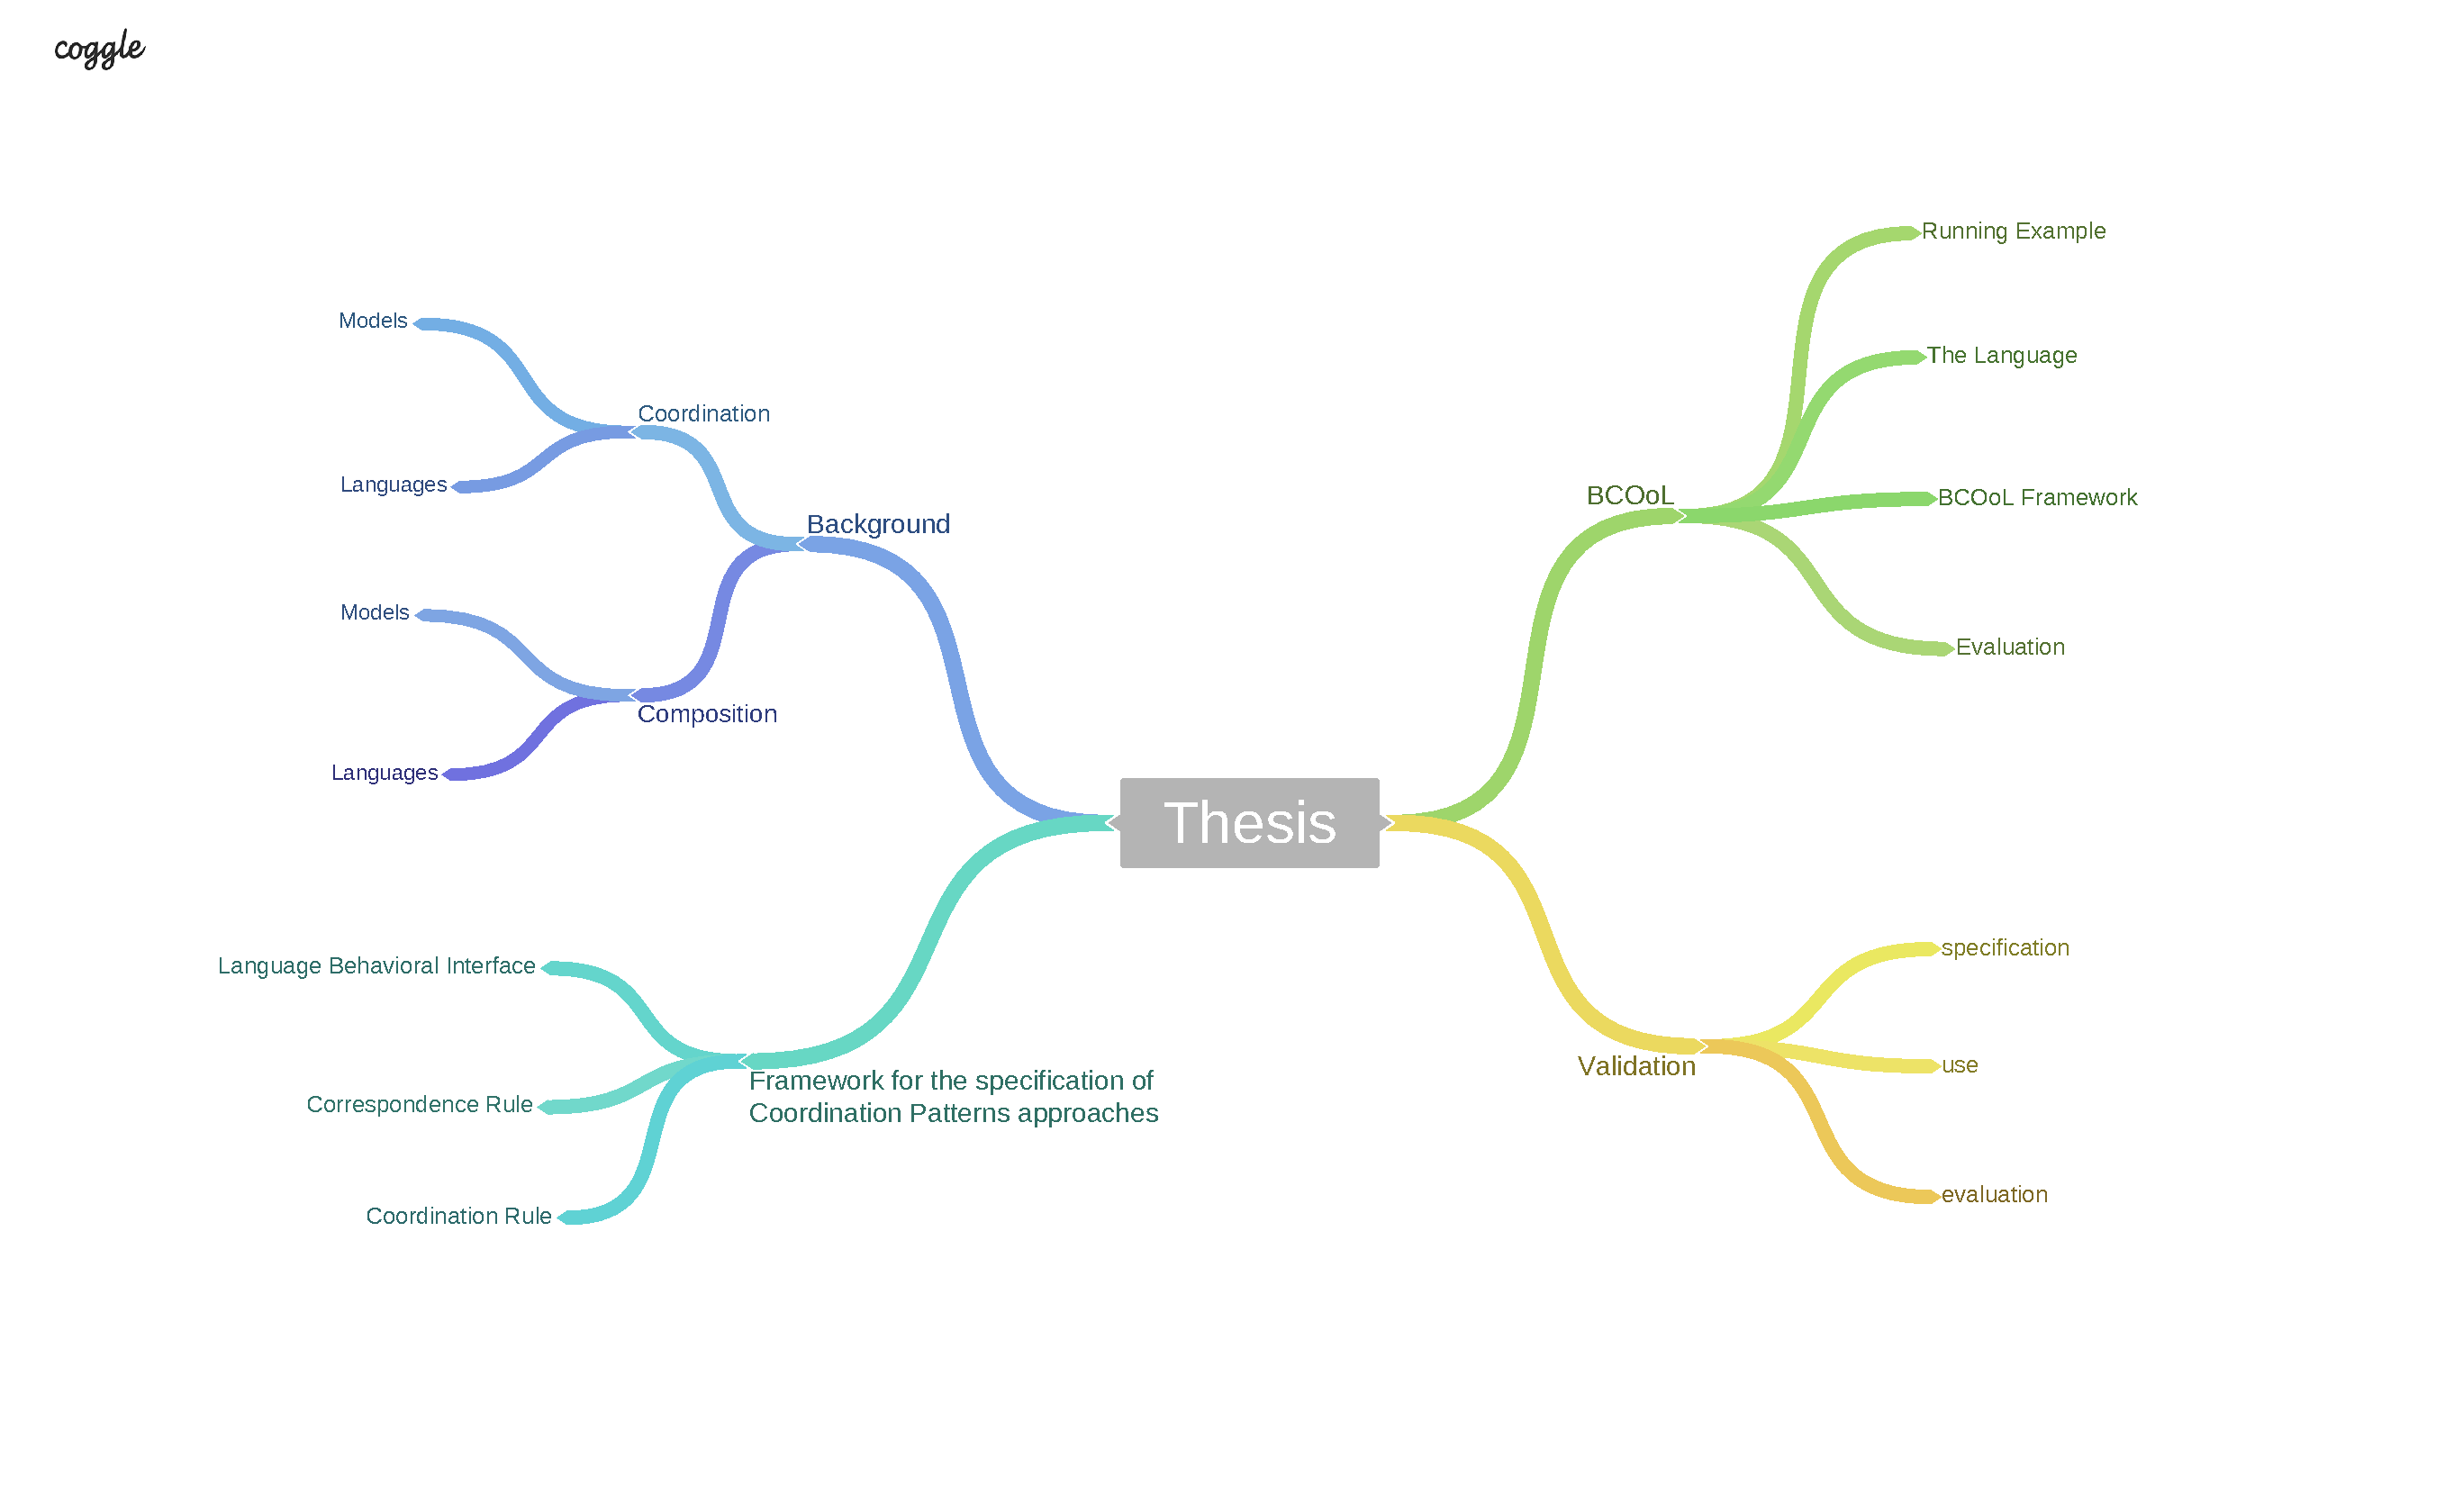
\includegraphics[width=1\textwidth]{Thesisoutline.pdf}
		\label{fig:thesis outline}
	\end{center}
\end{figure}
\end{landscape}

%\section{Problem}

%\section{Contributions}

%Contributions here.

%\section{Publications}

%Publications here.
\chapter{Background}
\label{ch:background}

\section{Introduction}
To deal with complexity issues in the development of applications for complex systems, Model Driven Engineering (MDE) proposes to rely on \emph{Models}. A model is an abstraction of the real world made in order to facilitate an understanding of the way it works. In the context of MDE, a software model enables a developer to reduce the complexity of an application by ignoring non-essential details. This enables the developer to reason about the application. 

The Object Management Group (OMG) proposes to specify models by relying on a language that has a well-defined form (syntax), meaning (semantics) and possible rules of analysis, inferences or proof for its constructs~\cite{mdaguide}. Thus, to build models, MDE proposes Domain Specific Modeling Languages (DSMLs). They are built by \emph{Language Engineers} to describe the structure but also the behavior of a particular domain. As a result, a DSML is defined by a syntax and a semantics. The syntax is described by a metamodel that defines the concepts and relations that the language is made up. A metamodel is a model that is developed by using a metameta language, \eg MOF, ECORE. To define the semantics, there are several approaches: Operational~\cite{operationbib}, Axiomatic~\cite{axiomaticbib} and Translational~\cite{translationalbib}. In this thesis, we focus on the description of the behavioral semantics of a language by relying on a Model of Computation (\mocc)~\cite{moccsemanticbib}. 

Based on a DSML, a domain expert builds a model to describe the structure and the behavior of a domain. However, the development of complex applications is often tackled by several domain experts. Each domain expert uses its own DSML to describe a part of the system. Thus, the use of several DSMLs results in a heterogeneous specification, \ie made of models that conform to different DSMLs. 

At some point of the development, a global representation of the system is needed to reason about the system as a whole. For instance, a system designer must be able to perform verification and validation activities of the overall system. Thus, it is necessary to specify how models and languages are related in a structural and behavioral way. 

This chapter presents the background in which this thesis relies on. We present different approaches to get a global representation of a heterogeneous system. We begin by presenting \emph{Composition Approaches} that propose to compose models/languages to obtain a new model/ language. We continue by presenting \emph{Coordination Approaches} that propose to specify the interaction between model/languages into and additional model so-called \emph{Model of Coordination}. By relying on these approaches, we conclude this chapter with the requirements for our language \bcool.  

%The development of complex software intensive systems involves interactions between different subsystems. For instance, embedded and cyber-physical systems require the interaction of multiple computing resources (general-purpose processors, DSP, GPU), and various digital or analog devices (sensors, actuators) connected through a wide range of heterogeneous communication resources (buses, networks, meshes).
%To deal with complexity issues in the development of applications for complex systems, Model Driven Engineering (MDE) proposes to rely on \emph{Models}. A model is an abstraction of the real world made in order to facilitate an understanding of the way it works. In the context of MDE, a software model enables a developer to reduce the complexity of an application by ignoring non-essential details. In this sense, The Object Management Group (OMG) defines that \emph{a model is a representation of a part of the function, structure and/or behavior of a system. The model specification is based on a language that has a well-defined form (syntax), meaning (semantics) and possible rules of analysis, inferences or proof for its constructs”}. This enables the developer to reason about the application. To built models, MDE proposes \emph{Domain Specific Modeling Languages} (DSMLs). They are built by an expert to describe the structure but also the behavior of a domain. As a result, a DSML, as any other language, is defined by a syntax and a behavioral semantics.  

%The development of complex applications may involve several DSMLs. Each expert uses its own language to describe its domain. This results in a heterogeneous specification, \ie made of models that conform to different DSMLs. Furthermore, nowadays systems are more and more coupled. As a result, system designers need to get a global representation to reason about the system as a whole. For instance, a system designer must be able to perform verification and validation activities of the overall system. To get a global representation, system designers need to combine models in a structural and behavioral way. In this thesis, we use the word \emph{composition} to refer to the combination of structural models/languages to obtain a new structural model/language. Conversely, we use the word \emph{coordination} to refer to the specification of the interactions between the behaviors of models/language into a new model, a so-called \emph{Model of Coordination}.   
 
%In this chapter, we first present an overview of composition approaches, which propose to compose the structure of models/languages to obtain a new model/language. Afterwards, we present state-of-the-art approaches that coordinate the behavior of languages/models. In these latter approaches, the interactions between languages/models are specified as a new model. By relying on these approaches, we conclude this chapter with the requirements for our language \bcool.        


\section{Composition Approaches}
\subsection{Overview}
Model composition is a modeling approach used in software engineering to combine models with a specific purpose. Clavreul~\cite{clavreulmodelcompo} defines model composition as the activity that ``\textit{enables to build a system from the union of independent or dependent software artifacts}''. A model is built based on a language that it is described by its meta model. A metamodel is a model that is developed by using a meta meta language, \eg MOF, ECORE. A metamodel has the concepts and relations to define a model.

Model composition proposes to specify \emph{correspondences} between the elements of the models (or meta-models) to be combined. Clavreul also identifies various \emph{interpretations} to these correspondences. An interpretation defines how the concepts are combined into a new model/language element. We rely on this vocabulary to analyze the state-of-art approaches. We categorize them into approaches that compose models and approaches that compose meta models. We name the former \emph{Composition of Model Approaches} and the latter \emph{Composition of Languages Approaches}.    

Composition of model approaches have as goal to get a resulting model that is built by combining one or more models of the same language or from different languages. The resulting model can conform to input models or to a different metamodel. In~\cite{mergemanifest}, authors identified that the composition between two models always relies on a \emph{merging} of structures. The merging is associated with an operator that takes two models as input and applies a \emph{relationship}. The relationship contains correspondences between model elements that defines \emph{what} elements must be composed. This approach proposes to automate the generation of correspondences by relying on a \emph{matching} operator that looks for syntactic similarities between models. From a set of correspondences, the merge operator generates a new model in which the matched elements are composed into a new element. In this work, authors suppose input and output models conform to the same language, however, they conclude that the framework could be extended to the heterogeneous case. By relying on this framework, authors have achieved to compare different approaches of model composition. However, they do not propose an implementation. 

\cite{kompose} also identified that the composition of models can be automated by relying on a matching and a merging operator. The matching operator specifies which concepts from different languages are related. The merge operator specifies how the matched elements are combined. The approach enables the system designer to specialize the operators to a meta metamodel. For example, they implemented it in a tool named Kompose which is based on the meta metamodel Ecore. Thus, the operators compose models that conform to different metamodels, but they conform to the same meta metamodel (\ie Ecore).

To ease the task of defining these operators, Epsilon~\cite{epsilon}\footnote{http://www.eclipse.org/epsilon/} provides dedicated languages to define both the matching and merging. The matching is specified in the \emph{Epsilon Comparison Language} (ECL) and the merging is specified in the \emph{Epsilon Merging Language} (EML). The ECL is used to define \emph{matching rules} that enable the developer to specify correspondences between concepts of two metamodels. Matching rules apply between models and select elements that must be combined. Then, the EML is used to define \emph{merging rules} that specify how the matched elements must be combined. This results in a new model. The metamodel of both the input models and the output models must conform to Ecore.

%\todo{To explain that the comparison is only between classes}

%\todo{To illustrate by using a Epsilon Specification}

The approaches previously studied only rely on structural similarities of the models to compose. While this works well with structural models such as class diagrams, it becomes a limitation when working with sequences diagrams. To produce a meaningful composition operator for sequence diagrams, the order in which events and messages have to be composed is based on the semantics of sequence diagrams. Thus, other approaches have concentrated on establishing semantic correspondences between models. They also rely on matching and merging operators, but they consider both structural and semantic information in the models.  

%The principal limitation of the proposed approach is that to be reusable the framework only relies on the structure of the models to compose. The signatures are the only elements which can be used to take into account some semantics of models to compose. Our current experiments show that it is not an issue when working with structural models such as class diagrams, database schemas or components model but it becomes a clear limitation when working with modelling languages such as sequence diagrams. 

Nejati et. al~\cite{compostatechartsbib} propose to represent the behavior of models by using statecharts. They propose an automatic approach to compose statecharts into a new statechart that represent the resulting behavior. The approach is based on a matching and merging operator. These operators rely on both structural and semantic information in the models. The matching operator is made of a combination of a \emph{static matching} and a \emph{behavioral matching}. The static matching identifies correspondence relationships between states by relying on theirs names. Thus, it is independent of the semantics of statechart and it is not different that the correspondence presented in the previous approaches. Conversely, the behavioral matching identifies correspondence relationships between states by relying on their behavior. For instance, the approach relies on measuring how close the behaviours of one state are to those of another. To do so, they compute a similarity degree for every pair of states by comparing the immediate neighbors of each pair of states. In this approach, a neighbor is either a successor/child states (forward neighbours) or a predecessor/parent states (backward neighbours). By relying on a static and behavioral matching, the matching operator returns a set of correspondence between states. Then, the merge operator takes as input two statecharts and the correspondences and generates as output an statechart model.
       
Aspect Oriented Modeling approaches~\cite{weavingbib} also consider the dynamic properties of models for the composition. However, in these approaches, the mechanism used to compose models is different. One model plays the role of \emph{base} and other the role of \emph{aspects}, both models conform to the same language. The composition of aspects into the base model is called \emph{weaving}. An aspect is made of a \emph{pointcut} and an \emph{advince}. The pointcut is a predicate over a model that is used to select relevant model elements called \emph{join points}. The join points are correspondence between the aspects and the base model. During the weaving, the join points are replaced by the advince, \ie the elements of a model (aspects), conform to a meta-model, are injected (woven) to another model that conforms to the same meta-model. In some approaches, the weaving of aspects is done by considering the behavior of the models used. For example, in~\cite{sequenceweavingbib,rambib,composdbib}, the behavior of a model is represented by a Sequence Diagram (base model). An aspect is defined as a pair of SD: one SD serves as a pointcut (specification of the behavior to detect), and one serves as an advice (representing the expected behavior at the join point). When a behavior in the base model is detected, the join point is replaced by the SD that represents the advince. The algorithm used for the weaving may vary from one approach to other thus resulting in a different SD depending the approach. 

%\todo{To illustrate by showing un example of weaving}

The previous approaches manage the composition of models in order to generate a new model. Conversely, composition of language approaches compose languages in order to generate a new language. In these approaches, the correspondences associate concepts of various metamodels in order to generate a new metamodel. The composition is done by a system designer that specifies \emph{what} and \emph{how} concepts from different metamodels are related. In the literature, several techniques exist that compose the structure of languages into a new language. For example, Emerson et al.~\cite{metamodelcompo} propose three of them:
\begin{itemize}
	\item \textbf{Merge:} The merging composes two languages that share a concept. These concepts are used as ``join points" to stitch the two languages together into a unified whole.
	\item \textbf{Interfacing:} When languages do not present joint points, the composition requires an interface. Thus interfacing composes languages that capture distinct but related domains by relying on an interface.
	\item \textbf{Refinement:} One language captures in detail a modeling concept that exists only as a ``blackbox" in a second DSML, \ie the concept defined in one languages refines in other in the second language.
\end{itemize} 
These techniques enable the composition of different languages by relying on the same meta meta model. For example, these techniques have been implemented in the GME framework~\cite{metamodelcompo}, which is based on the meta meta model MetaGME\footnote{http://w3.isis.vanderbilt.edu/projects/gme/meta.html}. The state-of-art approaches presents variation of these techniques. For instance, Monticore~\cite{monticore} propose two techniques: \emph{inheritance} and \emph{language embedding}. These techniques correspond respectively with refinement and interfacing. A different approach is Neverlang~\cite{neverlang} that enables to build a custom language from features coming from different General Propose Languages. A feature, such as the syntactical aspect of a loop, is encapsulated in a \emph{module block}. The blocks can be composed together for generating the compiler/interpreter of the resulting language. This approach can be understood as a ``interfacing" between general purpose programming languages.

These techniques only provide the means to compose the structure of languages. However, they make explicit neither the semantics of the language nor the semantics of the composition. Differently, \emph{Semantic Anchoring}~\cite{semanticsanchoring} proposes to explicitly define the behavior semantics of a language. Furthermore, it enables the definition of how the semantics can be composed in order to obtain a new semantics. To describe the behavioral semantics of a language, the approach relies on the concept of \emph{Semantic Unit} (SU). From authors, a SU is itself a language identified as ``basic", \eg Finite State Machine (FSM), Timed Automaton (TA) and Hybrid Automaton (HA). A SU is defined as a AsmL\footnote{http://research.microsoft.com/en-us/projects/asml/} specification in terms of (a) an AsmL Abstract Data Model (which corresponds to the abstract syntax), (b) the behavioral semantics (which is defined by the ASM mathematical framework). Then, the approach proposes to:
\begin{itemize}
	\item Define the syntax of a DSML by its metamodel. 
	\item Define the behavioral semantics of a DSML by specifying the model transformation rules between the metamodel of the DSML and the Abstract Data Model of a semantic unit. 
\end{itemize}    
The main benefice of the use of SUs is they can be composed into a new SU. For example, in~\cite{composemanticanch}, a SU named FSM (Finite State Machine) and a SU named SDF (Synchronized Data Flow) are composed to get a new SU called SU-EFSM. Roughly speaking, the composition is expressed manually using AsmL. Then, the resulting SU can be used to define the behavioral semantics of a language.

\subsection{Discussion}
Composition of Model approaches automate the composition between models by relying on a matching and merging operators. Furthermore, Epsilon eases the customization of operators by dedicated languages. The system designer can adapt the composition as needed. In these approaches, input and output models can conform to different metamodels, but they must conform to the same meta metamodel. However, these approaches can only specify the composition between two languages thus limiting its use in heterogeneous system. Besides, they only consider structural models thus ignoring their semantics.     

In~\cite{compostatechartsbib,weavingbib}, approaches have automated the composition of models by considering both syntactic and behavioral similarities. However, in these approaches, the composition is always specified between homogeneous models. Furthermore, operators are encoded inside a framework thus limiting the tunning of the specification. In addition, the detection of behavioral similarities between models is not easy or sometimes impossible as shown in~\cite{?}. 

Composition of Languages propose to model heterogeneous system by relying on a unified language. Such a language results from the composition of other languages. Unlike the composition of models, the composition of languages have not been automatized. Instead, a system designer has to 1) find correspondences between concepts of different languages and 2) specify how these concepts are related. This activity results in a new language. The inputs languages and the composed language are conformed to the same meta metamodel. In most of these approaches, correspondences are only between syntactic elements, and only one enables to define behavioral correspondences in order to obtain a new behavioral semantics. In this approach, authors state that its solution is to define semantics for heterogeneous DSMLs as the composition of semantic units. However, these approaches do not seem suitable for separation of preoccupation and development of a single system by various domain experts. 


%\section{Structural Composition Approaches}
In this section, we focus on the approaches that compose syntactic elements. We begin by approaches that propose to compose the syntax of models. They specify at language level how heterogeneous models can be composed, and then, they apply such specification to automate the composition of models. We finish this section with approaches that compose the syntax of languages into a new syntax. 

 	
 \subsection{Composition of Models Structure}

In this section, we overview approaches that compose the syntax of heterogeneous models into a single model syntax. They specify what concepts from different languages are selected and how they are composed. The specification is applied between models in order to generate a new model that may conform either to the inputs model languages (homogeneous case) or to a different language (heterogeneous case). In the following, we present the approaches by pointing on how they specify the composition.   

Brunet et al.~\cite{mergemanifest} identified that the composition of models always relies on a \emph{merging} operator. In this work, the merging operator takes two models as inputs and applies a \emph{relationship} which specifies how the models are related one to another. This results in a new model. In this work, authors suppose the models conform to the same language, but conclude that the merging operator can be generalized to heterogeneous models (if models conform to the same meta meta model). Several approaches like \emph{Kompose}~\cite{kompose} or \emph{Epsilon}~\cite{epsilon}\footnote{http://www.eclipse.org/epsilon/} rely on operators that are specified between languages but applied between models to generate a new model. 
    		
~\cite{kompose} relies on two generic operators to compose model: \emph{matching} and \emph{merging}. The matching operator specifies which elements in the language can match and how they can match. The merge operator defines how the matched elements are merged. The framework can be adapted to add composition capabilities to a particular language. For instance, Kompose adds composition capabilities to the Ecore metamodel. 
    		
Epsilon~\cite{epsilon}\footnote{http://www.eclipse.org/epsilon/} goes on step forward and purposes dedicated languages for specifying each operator. The matching operator is expressed by using the \emph{Epsilon Comparison Language}\footnote{http://www.eclipse.org/epsilon/doc/ecl/}. The merging operator is expressed by using the \emph{Epsilon Merge Language}\footnote{http://www.eclipse.org/epsilon/doc/eml/}. Theses languages are rule based oriented. The matching rules enable the user to specify a comparison algorithm to identify pairs of matching elements. The matching elements are merged through the merging rules. In this approach, both input models and output model must conform to the same meta meta model (Ecore).
    		
Different that previous approaches, \emph{Aspect Oriented Approaches}~\cite{aop} propose an asymmetric mechanism of composition where one model plays the role of \emph{base} on which other (partial) models named \emph{aspects} are woven. The aspect is made of a \emph{pointcut} and \emph{advice}. A pointcut specifies the \emph{join points} in the base model, \ie the place that will be replaced by the advice during the weaving. The advice contains the (partial) model that is to be woven. This approach is implemented in \emph{AspectJ}\footnote{http://eclipse.org/aspectj/}, \emph{MATA}~\cite{matabib} and \emph{SmartAdapter}~\cite{smartadapbib}. %In both approaches, an aspect is made up with a pattern matching and a composition specification. In SmartAdapter the composition specification is called composition protocol. The application of the aspect model to the base model is achieved in two phases. First, a match of the pattern has to be found in the base model. Once a match is found, the composition specification defines how elements are combined. Both tools are homogeneous approaches, \ie they compose models from the same language.       	

% sumarizes + link
The approaches previously studied specify the composition at language level in order to automate the composition between models syntax. In the next subsection, we overview approaches that specify the composition between languages in order to get a new language syntax. 	 		
    	
\subsection{Composition of Languages Structure}

Language composition approaches propose to compose the syntax of languages into a new syntax. A system designer specifies what concepts from different languages are related thus resulting in a new language. The characteristics of the new language depends on how languages are composed. Several techniques for language composition already exist. For instance, Emerson et al.~\cite{metamodelcompo} propose three techniques to compose the syntax of languages: \emph{Merging}, \emph{Interfacing} and \emph{Refinement}. The merging composes two languages that share a concept. These concepts are used as ``join points" to stitch the two languages together into a unified whole. However, when languages do not present joint points, the composition requires an interface. Thus interfacing composes languages that capture distinct but related domains by relying on an interface. In refinement, one language captures in detail a modeling concept that exists only as a ``blackbox" in a second DSML, \ie the concept defined in one languages refines in other in the second language. These techniques are implemented in the GME framework~\cite{metamodelcompo}. Monticore~\cite{monticore} is a similar approach that implements two techniques for the composition of languages: \emph{Inheritance} and \emph{Language Embedding}. These techniques, however, correspond respectively to refinement and interfacing in~\cite{metamodelcompo}.
	
Conversely, Nervelang~\cite{neverlang} is a framework that builds a custom language from features coming from general purpose languages. A feature, such as the syntactical aspect of a loop, is encapsulated in a \emph{module block}. The blocks can be composed together for generating the compiler/interpreter of the resulting language.  
	
%Also, it is not clear how much these approaches are suitable for separation of preoccupation and development a single system by various domain experts that focus on a specific part of the system.
	 	
\subsection{Discussion}
Composition language approaches tackled the problem of the heterogeneity of languages syntax by relying on a unified language, which is made by composing the syntax of other languages. In a complex system, where several languages are involved, a unique language may be hard to handle and reusability may be limited. Differently, composition models approaches specify the composition at language level but apply between models, thus resulting a new syntactic model. Such a specification seems easier to handle than whole language. 
			 	
The previous approaches only provide the means to compose syntactic elements. A modeling language has also a behavioral semantics that model the behavior of a domain. It is important to specify how different behavioral models interact in order to get the emerging system behavior. In the following, we present approaches that tackle the problem of the composition/coordination of heterogeneous behavioral models. 



%\section{Behavioral Composition Approaches}

In this section, we focus on approaches that deal with composition of behaviors. We categorize the state of art approaches into two groups. We begin by approaches that compose behavioral models. They specify the composition at language level, and then, they automate the composition of behavioral models (see Figure~\ref{fig:behacompomodel}). We finish this section by approaches that aim at compositing the behavioral semantics of languages into a new semantics.  

\begin{figure}
	\begin{center}
		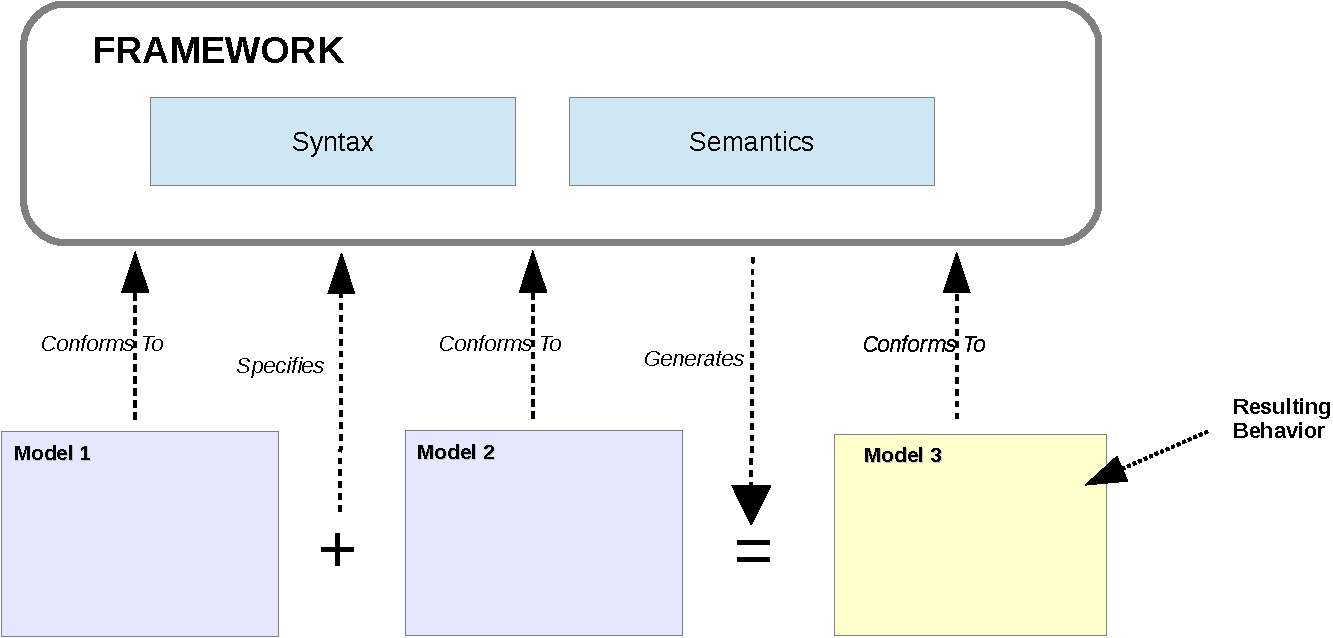
\includegraphics[width=.7\columnwidth]{background/figs/behacompomodel}
		\caption{Overview of Composition of Behavioral Models Approaches}
		\label{fig:behacompomodel}
	\end{center}
\end{figure}
	
\subsection{Composition of Behavioral Models}

In \cite{compostatechartsbib}, authors relay on statecharts to describe the behavior of models. Then, they propose an automatic approach to compose statecharts into a new statechar model. The resulting model represents the global behavior. The approach is based on a matching and a merging operator. The matching is used to produce correspondence relationships between states of two models. The matching can be \emph{static} and \emph{behavioral}. The static matching is based on a naming convention thus relying on the syntax of statechart. Conversely, the behavioral matching selects pair of states by relying on their behavioral semantics. The merging operator takes as input two models and a correspondence relation, and it generates a new model conforming to statecharts that represents the global emerging behavior. This approach is implemented in a tool named TReMer~\footnote{https://se.cs.toronto.edu/index.php/TReMer\%2B}. %A similar approach is presented in~\cite{compoclassdiagrambib}. However, in this approach, authors represents the behavior of models by using se   
		 
Aspect Oriented Modeling provides a different approach through the weaving of aspects that encapsulate behaviors~\cite{weavingbib}. Advices represent a new behavior that should replace the base behavior when it is matched by the pointcut. For instance, in AspectJ~\cite{AspectJoverview}, the aspects are used to extend Java and the advice is expressed in Java code. Similarly, RAM~\cite{rambib,composdbib} is an aspect oriented approach in which the behavior of aspects is described by using sequence diagrams. The approach proposes the composition of behavioral models by relying on the weaving of sequence diagrams.

The previous approaches specify how behavioral models can be composed into a new model that represents the resulting system behavior. In the next subsection, we overview approaches that specify how the behavioral semantics of languages can be composed into a new semantics.

\subsection{Composition of Language Behavioral Semantics}
To our knowledge, only Chen et al.~\cite{semanticsanchoring} propose to define the semantics of a language by composing other semantics. In this work, a \emph{Semantic Unit} (SU) is represented by a structure (\emph{Abstract Data Model}) and a behavioral semantics. The approach specifies the SU in the \emph{Abstract State Machine Language}\footnote{http://research.microsoft.com/en-us/projects/asml/} (Asml). This language is used to specify both the structure and the semantics of a SU. A given SU is associated to the Abstract Syntax (AS) of a language through a mapping. The mapping associates each element in the AS with an element in the Abstract Data Model of the SU. This approach  enables the system designer to compose two SU into a new one. For instance, in~\cite{composemanticanch}, authors define two SU named Finite State Machine (FSM) and Synchronize Data Flow (SDF), and then, they specify how the two SU can be composed into a new one called EFSM.  

\subsection{Discussion}
Composition of Behavioral Models approaches rely on a common semantics to describe the behavioral of models. Then, they automated the composition of behavioral models by relying on a set of rules at language level. In~\cite{semanticsanchoring}, authors also rely on a common semantics to describe the behavioral semantics of languages (\eg Asml) and a set of rules between semantics elements. However, these rules specify how the semantics of languages can be composed into a new semantics. In a complex system, where heterogeneous languages may be used, a unified language could be hard to handle thus limiting the reusability.
In the following section, we study approaches that propose to coordinate behavioral models instead of compose them.  

\section{Coordination Approaches}
\subsection{Overview}
To be executable, each DSML defines a behavioral semantics. The specification of the behavior semantics of a DSML varies from natural language to the use of a formal language. In any case, the developing of complex applications relies on heterogeneous DSMLs thus resulting in heterogeneous behavioral models. In this context, Model coordination is a modeling approach to integrate the behavior of models. It proposes to specify the interaction between heterogeneous behavioral models by relying on a \emph{model of coordination}. According to \cite{coordsignibib}, ``\textit{Coordination is the process of building programs by gluing together active pieces}''. In this thesis, we adopt the wording of \emph{coordination} as being the explicit modeling of the interactions amongst behavioral models to obtain the emerging system behavior. In this sense, the coordination must be executable to enable the evaluation of the emerging behavior of the whole system. 

The goal of the coordination is the integration of behavioral models. Clavreu~\cite{clavreulmodelcompo} stated two commons issues in the integration of systems: 
\begin{itemize}
	\item The models are developed independently by relying on different technologies.
	\item It is very often forbidden to modify existing systems to implement the integration.   
\end{itemize}
In this context, Coordination approaches propose to define the interactions between models separately from the computation. As a result, the existing models are not changed and the coordination only constraints theirs behaviors. 

In this section, we present an overview of approaches that coordinate the behavior of models and languages. We categorize them into \emph{Coordination Languages and Architecture Description Languages}, and \emph{Coordination Frameworks}. The former enables a system designer to model the coordination between models whereas the latter provides a tool to automate the coordination of heterogeneous models by specifying the coordination between heterogeneous languages.

Coordination Languages have been proposed by Carriero et al.~\cite{coordsignibib} in order to model the coordination between heterogeneous behavioral models. Depending the entities coordinated, approaches can be categorized into \emph{data-driven} or \emph{control-driven}. The former coordinates data between models whereas the latter coordinates events between models. Arbab~\cite{whatdocoord} propose to classify the approaches into \emph{endogenous} and \emph{exogenenous} languages. An endogenous language provides coordination primitives that must be incorporated within a model for its coordination. For instance, Linda~\cite{lindabib} provides a set of primitives like \emph{in()} or \emph{out()} to exchange data between models. These primitives must be added to a host language by using libraries. 


%Some coordination languages deal with the complexity of model behaviors by treating models as black boxes encapsulated within the boundary of an interface. A model behavioral interface gives a partial representation of the model behavior therefore easing the coordination of behavioral models. However, it is not uniquely defined and may vary depending on approaches. For instance, in \emph{Opus}~\cite{Opus}, the interface is a list of methods provided by the model. Other approaches abstract away the non-relevant parts of the behavior of models as events~\cite{eventStructures} (also named signals in~\cite{lee1998framework}). These approaches focus on events and how they are related to each other through causal, timed or synchronization relationships. Following the same idea, \emph{control-driven} coordination languages rely on a model behavioral interface made of explicit events~\cite{rapide,esperbib,coordinainterfacebib}. While in Rapide~\cite{rapide}, the interface is only a set of events acceptable by the model, some other approaches go further and also exhibit a part of the internal concurrency. This is the case of~\cite{coordinainterfacebib} where authors propose an interface that contains services and events, but also properties that express requirements on the behavior of the components. Such requirements act as a contract and can be checked during the coordination to ensure a correct behavior. In these approaches, the model behavioral interface provides information to coordinate the behavior of a model.



Conversely, exogenous coordination languages deal with the complexity of model behaviors by treating models as black boxes encapsulated within the boundary of an interface. A model behavioral interface gives a partial representation of the model behavior therefore easing the coordination of behavioral models. The coordination is thus specified between elements of the interface. The notion of interface varies depending on the approach. For instance, in \emph{Opus}~\cite{Opus}, the interface is a list of methods provided by the model. Other approaches abstract away the non-relevant parts of the behavior of models as events~\cite{eventStructures} (also named signals in~\cite{lee1998framework}). These approaches focus on events and how they are related to each other through causal, timed or synchronization relationships. Following the same idea, \emph{control-driven} coordination languages rely on a model behavioral interface made of explicit events~\cite{esperbib,manifoldbib,coordinainterfacebib}. While in Esper~\cite{esperbib}, the interface is only a set of events acceptable by the model, some other approaches go further and also exhibit a part of the internal concurrency. This is the case of~\cite{coordinainterfacebib} where authors propose an interface that contains services and events, but also properties that express requirements on the behavior of the components. Such requirements act as a contract and can be checked during the coordination to ensure a correct behavior. The benefices of event driven coordination languages are twofold:
\begin{itemize}
	\item They give support for control and timed coordination while remaining independent of the internal model implementation.
	\item They coordinate models without any change to their implementation, thus ensuring a complete separation between the coordination and the computational concerns.
\end{itemize} 


\todo{ADLs are based on the idea to keep computation and coordination as different concerns. They are control drive coordination languages (exogenenous). In this aproaches, the concepts of interfaces and connector become very important}

In parallel, the \emph{software architecture} research field dealt with the growing complexity of software system by proposing languages (named ADL for Architecture Description Languages) to gain abstraction, structuring and reasoning capabilities~\cite{rapidebib,wrightbib,uniconbib,frameadlsbib,garlansoftarchbib}. An ADL usually specifies a system in terms of \emph{components} and interactions among those components. They enable a system designer to:
\begin{itemize}
	\item Clarify structural and semantics difference between components and interactions.
	\item Reuse and compose architectural elements.
	\item Identify/enforce commonly used patterns (\eg architectural styles).
\end{itemize}
Depending on the ADL, a \emph{Component} can for instance be an encapsulation of some procedure, an encapsulation of an object file or a (formal) abstraction of its behavior. To externally characterize the components, ADLs rely on well identified \emph{Component Interfaces}. The interfaces are used by \emph{Connectors} whose behavior is specified by a \emph{glue}. Connectors can represent a large variety of interactions (\eg procedure call, event broadcast or database queries) and the glue can range from a simple function to complex protocols. 

Both coordination languages and ADLs make a clear separation between two design activities: the specification of the component (\ie the computational aspects) and the assembly of these components (\ie the communication/coordination aspects). While the first activity is usually done by a software engineer, the second one is done by a system designer. He has to deal with the architecture-level communication that is expressed with complex protocols. To abstract away these protocols and make them reusable, ADLs propose connectors as types~\cite{frameadlsbib} that can be used on the shelf to specify domain specific interactions.

For example, Clara~\cite{clarabib} is an ADL dedicated to real time systems. It proposes built-in connector types like \emph{Rendez-vous}, \emph{Mutex} or \emph{Mailboxes}. This helps the task of a system designer by providing relevant domain specific connectors. However, this also limits what can appear in the interaction. 

Other approaches introduced the notion of \emph{user defined type}~\cite{uniconbib,wrightbib,reobib} that enables a system designer to build connectors for an specific domain. A connector type is defined by a set of \emph{roles} and a \emph{glue specification}. Roughly speaking, a role represents a formal parameter that is used to specify the glue. The glue is based on a formal language to specify how roles are coordinated. For instance, in Wright~\cite{wrightbib}, the glue is specified in a variant of CSP~\cite{csphoarebib}, whereas in Reo it is specified by the composition of dedicated primitives~\cite{reobib}. The connector types are later on instantiated and the roles are bound to the actual interfaces of the instances of components. 

\begin{figure}
	\begin{center}
		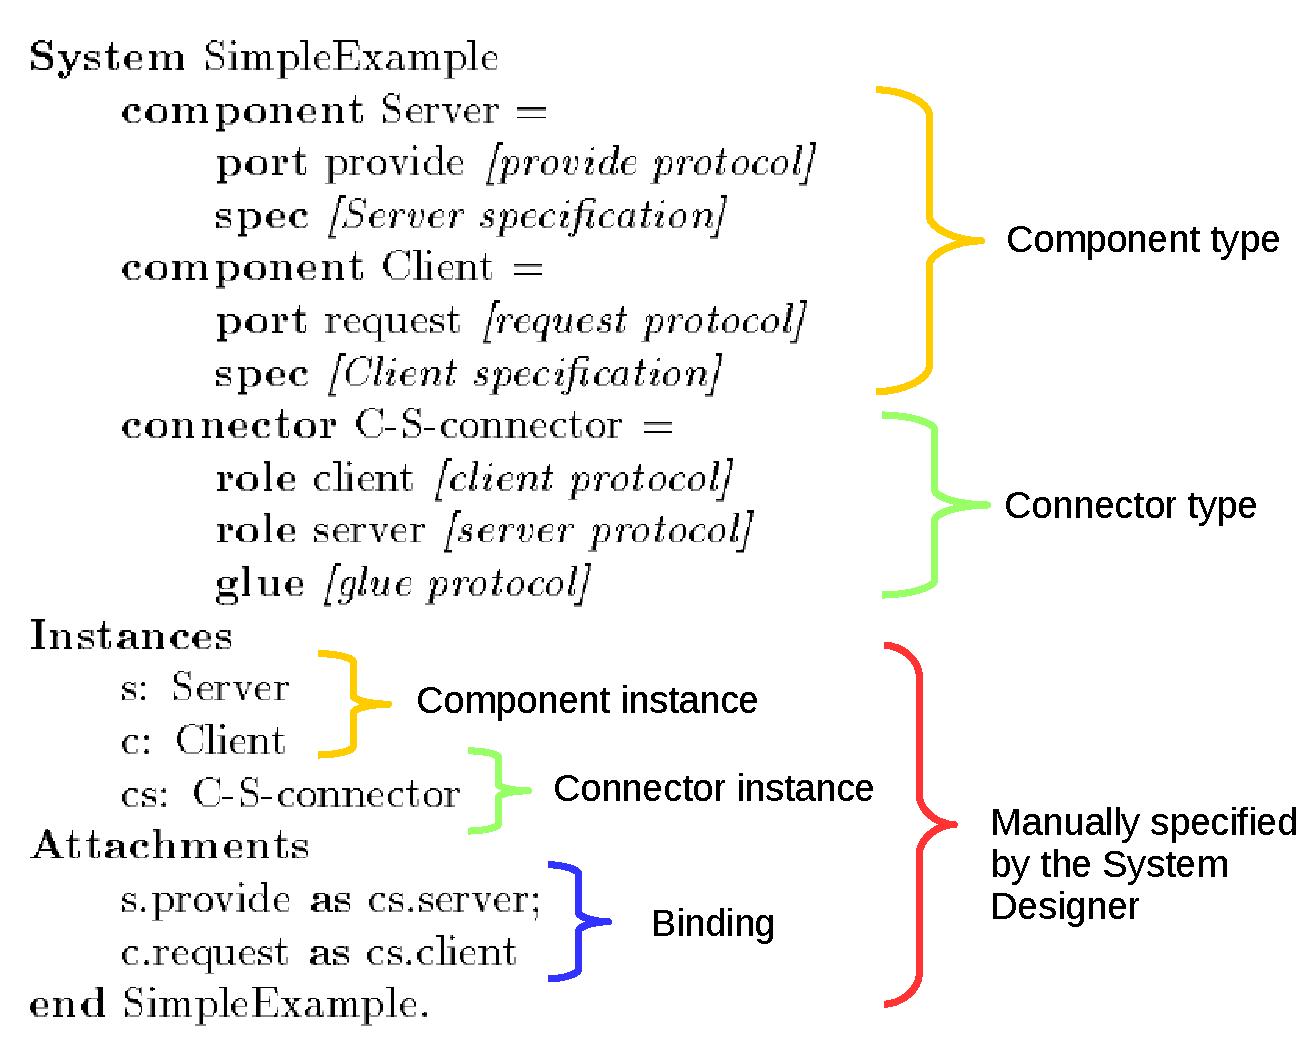
\includegraphics[width=0.5\textwidth]{background/figs/wrightspec}
		\caption{Specification of a Client-Server system in Wright~\cite{wrightbib}}
		\label{fig:wrightspec}
	\end{center}
\end{figure}

To illustrate how a system designer can define a set of domain specific connector types, Figure~\ref{fig:wrightspec} shows a simple client-server system described in Wright~\cite{wrightbib}. The specification defines two component types named \emph{Client} and \emph{Server}, and one connector type named \emph{C-S-connector}. The C-S-connector has two roles (\emph{client} and \emph{server}) and a glue that describes how the activities of the client and server roles are coordinated. The section \emph{Instances} describes a particular configuration by instantiating the corresponding components and connectors. The example describes a system where there is a single server (\emph{s}), a single client (\emph{c}) and a single connector (\emph{cs}). Then, the section \emph{Attachments} defines which component ports are attached to the connector roles. ADLs have successfully identified the need of connector types in order to ease the task of a system designer. In~\cite{wrightbib}, authors claim that connector types enables to ``\emph{understand a general pattern of interaction that can occur many times in any given system}''. Thus, a system designer has only to instantiate and bind connector types as needed by its architecture. 

The major drawback of coordination languages and ADLs is that the specification of the coordination is between particular models. For example, in the case of ADLs, a system designer has to instantiate and bind connector types manually. Returning to the example of Figure~\ref{fig:wrightspec}, for each server and client in the system, the system designer has to instantiate two components and one connector. Then, he has to bind the component ports with the connector roles. With the increasing number and heterogeneity of the components, this task can quickly become difficult and error prone.

\emph{Coordination Frameworks} identified that the instantiation and binding of connector types can be a systematic activity the system designer repeats many times and can consequently be defined as a pattern. Such a pattern is based on the \emph{know-how} of the system designer and sometimes on naming or organizational conventions adopted by the models. Thus, they have captured the specification of a \emph{behavioral coordination pattern} inside a tool/framework to automate the instantiation and binding of connector types. In these approaches, the coordination is specified between heterogeneous languages rather than between particular models. 
\begin{figure}
	\begin{center}
		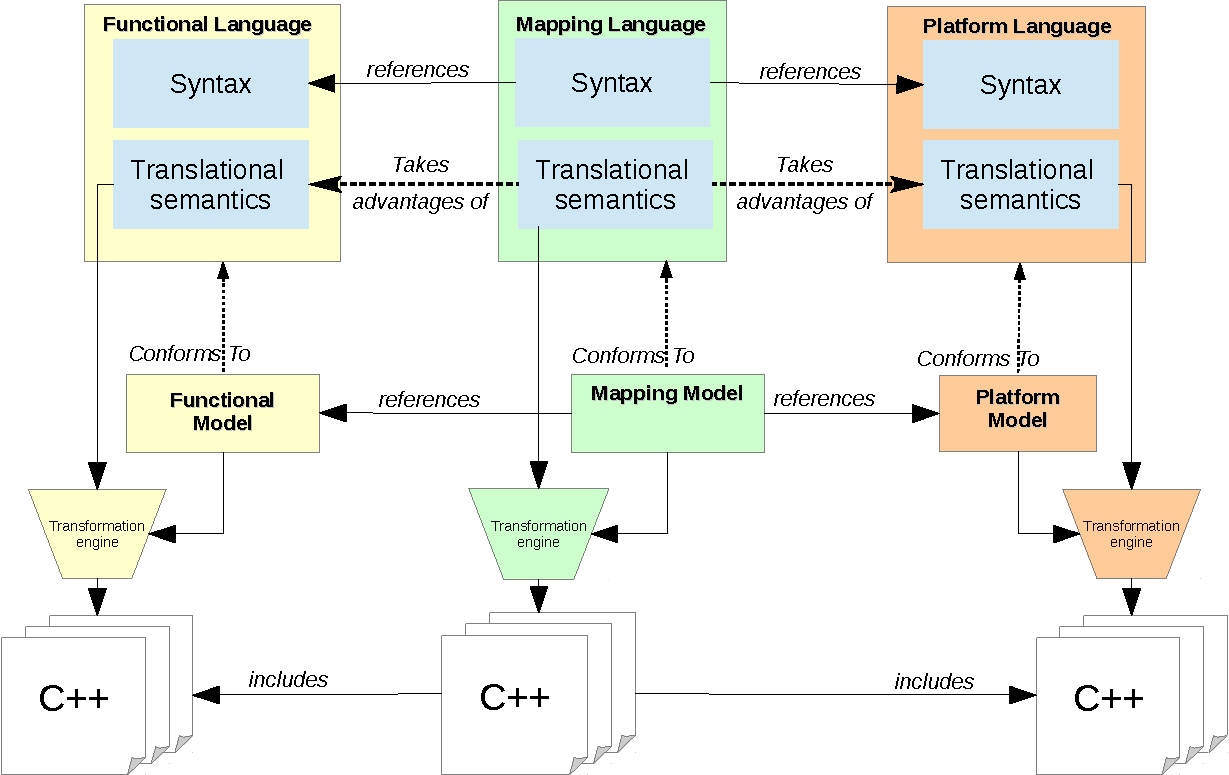
\includegraphics[width=0.7\textwidth]{background/figs/diNatale}
		\caption{High Level view of the approach proposed by Di Natale et al. in~\cite{dinatale}}
		\label{fig:diNatale}
	\end{center}
\end{figure}
% maltab and sdl has a sintax but also a semantics coompletly different. 
% matlab is data flow (sdf) y sdl (control flow or fsm)
% matlab vectores de datos, sdl events. 
% implementa como sincronizar eventos con datos

For example, MASCOT~\cite{mascotbib} is an approach focused on the integration of Matlab~\cite{matlabbib} and SDL~\cite{sdlbib}. Whereas SDL is a language suitable for control systems modeling, Matlab is better for modeling dataflow aspects of a system. However, these languages are very different, while SDL processes operate on events, represented by simple signals, Matlab processes operate on vectors, represented by vectorized signals. Thus, authors propose to automate the synchronization of control signals from SDL with data signals from Matlab. These signals can be either notification signals or message signals. Notification signals do not carry a value and are used to notify a process that an event has occurred. Message signals carry a value and are used to indicate a change of some variable or parameter. The approach deals with the integration of the timing and synchronization concepts from both languages by proposing two synchronization modes: head synchronization and tail synchronization. These mechanisms take advantages of the knowledge about the semantics of the languages. For instance, in the head synchronization, when a model in matlab receives a frame \emph{a1}, it immediately transforms \emph{a1} into \emph{b1} (dataflow network model). Any control signal from SDL that occurs during the transformation of \emph{a1} to \emph{b1} cannot influence its value. Then, the head synchronization mode ensures that the occurrence of the control signal is taken into account when the next frame is processed. In the tail synchronization, when a model in Matlab receives a control signal from SDL, the signal is collected until it cease to occur, then, it is translated to a vector and passed to the Matlab model. The modes of synchronization ensure the communication between Matlab and SDL. In addition, the approach gives a set of guidelines to aid the system designer to choose between the two synchronization proposed. Once the synchronization policy is defined, the approach enables the co-simulation of a SDL model and a Matlab model. The implementation is based on SDL wrappers. A process in the SDL specification that is specified in Matlab contains a wrapper that interfaces between the SDL simulator and the Matlab engine. A SDL wrapper is made of a set methods that enable the SDL engine to control the behavior of the data signals in Matlab. To do so, the approach relies on the name of signals in SDL specification to communicate with the signals in Matlab. The approach thus forces the system designer to follow a naming convention between signals in both domains. Although the current implementation partially automates the coordination of signals from both domains, the approach has identified and captured a coordination pattern between a control-flow language and a data-flow language by relying on some knowledge about its syntax and semantics.

In~\cite{dinatale}, authors deal with the integration of a language to describe the functional aspects and a language to describe the platform by proposing a dedicated mapping language. The mapping language syntax references syntactic elements from both the functional and the platform language. For instance, the $SWdeployment$ concept from the mapping model, references the $Task$ concept from the functional model and the $CPU$ concept from the platform model. Based on the mapping model, the approach generates the code of the communication between the functional and platform models. The semantics of both the functional and the platform language is defined by an translational approach into C++ code. The translational semantics of the mapping language takes advantages of some knowledges about the translational semantics of the other languages. For instance, for each subsystem in the functional language, authors know that a class is generated with name \emph{SubsystemName}\texttt{ModelClass}. They also know that the class has a \texttt{step} operation for the runtime evaluation of the block outputs given the inputs and the state. Thus, from a mapping model, the approach can generate the code to communicate a functional and platform model. The approach proposes a set of connectors that the system designer has to instantiate in the mapping model. In this sense, it is similar than others ADLs that propose a set of built-in connectors. However, different than other ADLs, connectors types link concepts from the syntax of languages. In particular, these connectors capture some knowledge of a system designer that performs the mapping of a functional model to a platform model. 
 
%The semantics of both the functional and the platform language is defined by an translational approach into C++ code. 

%This approach has achived to: 1) propose a dedicated language to explicitly relate concepts from both languages. Such a language contains as a built-in connector types that the developer can instantiate. 2) From such connectors, a generative approach enables to generate the comunication code in C++. 



%A first interesting aspect of this approach comes from the possibility, by creating a dedicated language, to reuse existing languages, and based on a mapping model to automatically generate the glue between the implementation of the models (in this case encoded in C++). 

%The mapping language syntax references syntactic elements from both the functional and the platform language. For instance, the $SWdeployment$ concept from the mapping model, references the $Task$ concept from the functional model and the $CPU$ concept from the platform model. 


%The translational semantics of the mapping language takes advantages of some knowledges about the translational semantics of the other languages. For instance, for each subsystem in the functional language, authors know that a class is generated with name \emph{SubsystemName}\texttt{ModelClass}. They also know that the class has a \texttt{step} operation for the runtime evaluation of the block outputs given the inputs and the state. 

%In other words, authors have a partial but sufficient knowledge of the translational semantics of both the functional and the platform language. 

%Finally, based on this knowledge, they encode in the translational semantics the glue to generate according to the actual mapping in the mapping model. 

 \begin{figure}
 	\begin{center}
 		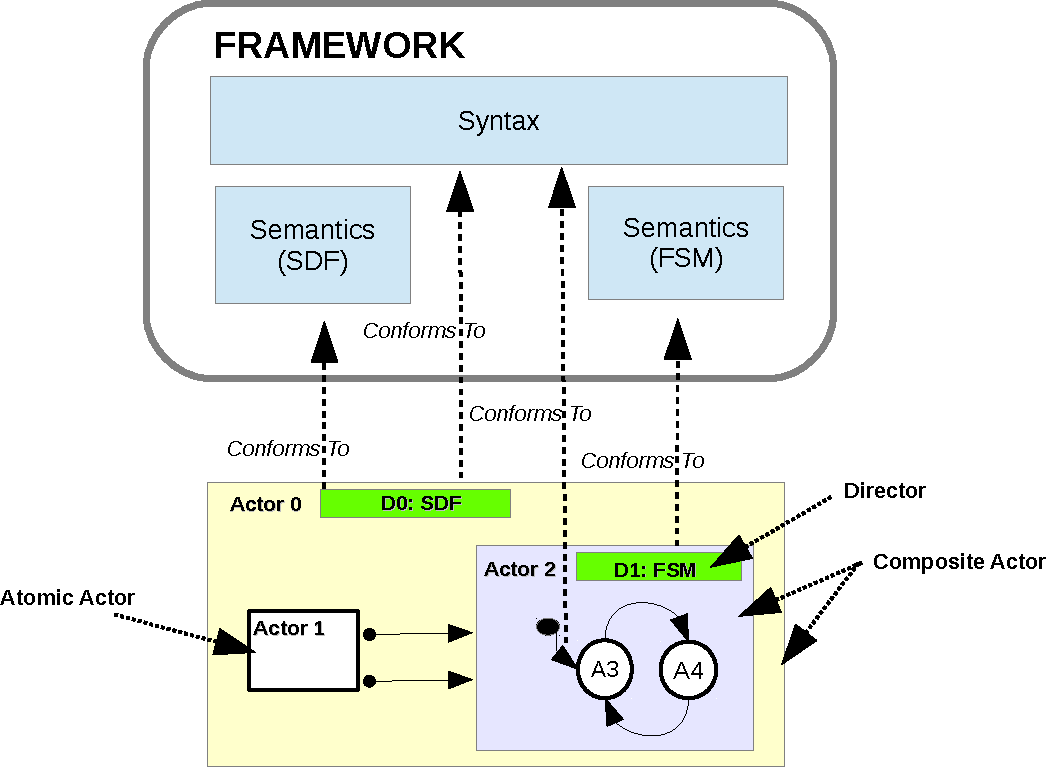
\includegraphics[width=0.7\textwidth]{background/figs/ptolemyfig}
 		\caption{High level view of Ptolemy~\cite{giraultbib}}
 		\label{fig:ptolemyfig}
 	\end{center}
 \end{figure}
 
 While the previous approaches are ad-hoc solution for two particular languages, Ptolemy~\cite{ptoleframebib} and ModHel'X~\cite{modhelxbib} are systematic approaches to coordinate models that conform to a set of predefined languages. These approaches rely on framework in which the syntax of models is described by actors and the semantics is given by a Model of Computation (MoC). Actors can be atomic (\eg \emph{Actor 1} in Figure~\ref{fig:ptolemyfig}) or composite (\eg \emph{Actor 0} and \emph{Actor 2} in Figure~\ref{fig:ptolemyfig}), \ie made of internal actors. Each composite actor has associated a model of computation that defines a \emph{Domain}. A domain specifies the communication semantics and the execution order among internal actors. A domain is implemented by a \emph{Director}. For instance, in Figure~\ref{fig:ptolemyfig}, the \emph{Actor 0} has the director \emph{D0} that follows the semantics of SDF and the \emph{Actor 2} has the director \emph{D1} that follows the semantics of FSM. In this approach, actors, both atomic and composite, are executable. In a composite actor, the execution order of internal actors is controlled by a director. In the example of Figure~\ref{fig:ptolemyfig}, the director \emph{D0} controls the execution of the \emph{Actor 1} and \emph{Actor 2} and director \emph{D1} controls the execution of \emph{A3} and \emph{A4} whenever \emph{Actor 2} is executed. In this sense, the execution of composite actors is strictly hierarchical. The behavior of actors is represented by a generic interface that contains a set of methods, \eg fire(). The MoC implemented by the director of a composite actor specifies when the methods in the interface of internal actors are invoked. For instance, when a composite actor is fired, the director associated with the composite actor fires the actors of the contained model. Based on a fixed syntax and a generic interface, these approaches have achieved to capture a hierarchical coordination pattern into a framework. The framework provides a dedicated syntax to specified the pattern, \ie composite actors, and encodes the necessary glue between interfaces to coordinate their execution. 
 
\subsection{Discussion}
Coordination languages and ADLs enable the system designer to define one or more models of coordination to specify how behavioral models interact. The main benefice of these approaches is that the global behavior is explicit and amenable for reasoning (for instance for Verification and Validation activities). Furthermore, they propose languages closed to system designer domain. For example, ADLs provide types in order to define domain specific connectors.  

These approaches have successfully identified connectors type, however, a system designer has still to specify when a type of connectors is used. He has to manually instantiate them by relying on his know-how. In a complex system, such a task can quickly become tedious and error prone. Furthermore, if one of the model changes, the model of coordination must also be changed. By relying on Coordination Languages and ADLS, a system designer only captures the solution for one single problem but he is not able to specify a systematic way to coordinate models. 

Conversely, Coordination frameworks have achieved to capture the know-how of a system designer by specifying coordination patterns. Such specification at language level allows automating the coordination between behavioral models. However, they embed the coordination pattern inside a tool. This has two major drawbacks:
\begin{itemize}
	\item 1) Validation and verification activities are limited since the coordination is encoded by using a general purpose language (\eg Java in Ptolemy and ModHel'X).
	\item 2) The system designer cannot change the proposed coordination without altering the core of the tool. 
\end{itemize} 
Regarding the point number one, coordination languages and ADLs have already tackled this problem by using a formal language to express the coordination (\eg CSP in Wright). This enables providing verification and validation of the coordinated system. Recent work in that direction is presented in~\cite{semanticadaptccsl} where CCSL~\cite{ccslbib} is used to specify the semantic adaption in ModHel'X. 

Concerning the point number two, for complex systems, the system designer may need to capture several coordination patterns and potentially combine them. However, current coordination frameworks can only support such a variation by modifying the framework itself. The coordination model is mixed with the functional model, which makes it very tricky to modify one without risking altering the other.

To summarize, the achievement of coordination approaches are:
\begin{itemize}
	\item To become the interaction between behavioral models explicit and formal. 
	\item To leverage on the system designer know-how by capturing coordination patterns. 
\end{itemize}

%\section{Behavioral Coordination Approaches}

\todo{In these approaches, the emerging behavior is obtanied by specying a model of coordination. A model of coordination defines how different models interact.}
\todo{We categorize these approaches into \emph{Coordination Languages} and \emph{Coordination Frameworks}. The former aims at specifying the coordination between models while the latter aims at specify the coordination between languages in order to generate the coordination between models.}

\subsection{Coordination of Models}

\begin{itemize}
		    \item These approaches propose to coordinate the behavior of heterogeneous models. The specification is done by a system designer that uses either a \emph{Coordination Language}~\cite{coordmodels} or an \emph{Architecture Description Language}~\cite{frameadlsbib}. This process results in the specification of a model of coordination. 
			 
			\item Coordination language approaches focus on the development of parallel and multilingual systems by separating the computation concerns from the coordination concerns. They provide a dedicated language (\eg Esper~\cite{esperbib}, Linda~\cite{lindabib}, Manifold~\cite{manifoldbib}) for the specification of the interaction between different parts of the system. According to \cite{coordsignibib}, ``\textit{Coordination is the process of building programs by gluing together active pieces}''. A system designer defines one or more coordination model(s) to specify how the system models interact with each other. In~\cite{wegnercoorbib}, authors highlighted that the design of coordination languages must address the following issues: identification of the entities to coordinate, architecture style of the coordination and protocols/rules of coordination.
			 
			\item During the same period, the \emph{software architecture} research field dealt with the growing complexity of software system by proposing languages (named ADL for Architecture Description Languages) to gain abstraction, structuring and reasoning capabilities~\cite{rapidebib,wrightbib,uniconbib,frameadlsbib,garlansoftarchbib}. An ADL usually specifies a system in terms of components and interactions among those components. Such languages helped 1) to clarify structural and semantics difference between components and interactions, 2) to reuse and compose architectural elements, 3) to identify/enforce commonly used patterns (\eg architectural styles). There now exist many ADLs, with specific goals and domains. Depending on the ADL, a \emph{Component} can for instance be an encapsulation of some procedure, an encapsulation of an object file or a (formal) abstraction of its behavior. Most of the ADLs in the literature rely on well identified \emph{Component Interfaces} to externally characterize the components. The interfaces are used by \emph{Connector}s, whose behavior is specified by a \emph{glue}. The connectors can represent a large variety of interactions (\eg procedure call, event broadcast or database queries) and the glue can be of very different complexity ranging from the identity function to complex protocol specification. 
			 
			
			\item BIP~\cite{bipbib} specifies the coordination or \emph{interactions} between \emph{components} by using \emph{connectors}. The approach provides a minimalist but expressive and formal algebra to specify the coordination between different automaton thus allowing the user to check properties like dead-lock freedom. Similarly, Metro2~\cite{metro2bib} relies on connectors and ports. However, while Metro2 enables to coordinate heterogeneous components, in BIP the components can only encapsulates automaton models. 
			 
			 
			\item \emph{CyPhyML}~\cite{semanicbackplane} is a language aimed at integrating models that can conform to heterogeneous modeling languages, \eg SySML, AADL. As authors state, it is an \emph{Integrated Models Language}. In this approach, the semantics of modeling languages is abstracted by using a semantic interface which contains the essential concepts for cross-domain integration. By using semantic translators, models are transformed into CyPhy model integration space according to their semantic interface~\cite{semanicbackplane}. Then, CyPhy is used to specify the integration between models. The specification is written in FORMULA thus providing verification and analysis of the integrated system. In CyPhy, the coordination is specified between particular models, in this sense, CyPhy remains a coordination language.
			 
			
			%\item \todo{ForSyde methodology~\cite{forsydebib} is a different approach, where the behavioral of a system is captured by a fixed formal model of computation. The formal model is described following the denotational framework of Lee and Sangiovanni-Vincentelli~\cite{frameworkleebib}. A system is network of process that communicates thought signals. The specification model is based on a synchronous computational model. The specification model is expressed in the functional programming language Haskell.}
			
			\item Coordination languages and ADLs have common objectives~\cite{coordmodels}. They build/understand/analyse a system based on ``components'' (possibly written in different languages) and connectors (which include the specification of the interaction/coordination). Furthermore, they make a clear separation between two distinct activities in the development of a system: the specification of the different component of a system (\ie the computational aspects) and the assembly of these components (\ie the communication/coordination aspects). The first activity is usually realized by a software engineer and the second one is realized by a system designer. The system designer has to deal with the architecture-level communication that is often expressed with complex protocols. To abstract away these protocols and make them reusable, ADLs help the system designer by proposing connectors as types~\cite{frameadlsbib}. The main objective of that is to provide on the shelf connectors with domain specific interactions between components. 
			
			\item Approaches like AADL~\cite{aadlbib} or Clara~\cite{clarabib} (to cite only two of them) proposed built-in connector and component types. These built-in types can either be part of the ADL or part of the architectural style (more details are provided in~\cite{taxonomyConnectors}). Providing built-in connector types reifies interesting interactions, usually according to a specific domain. For instance, the Clara ADL is dedicated to real time systems, consequently it proposed built-in connector types like \emph{Rendez-vous}, \emph{Mutex} or \emph{Mailboxes}. This reification of coordination helps the coordination tasks by providing relevant domain specific constructions. It also limits what can appear in the interaction and is a step towards providing domain specific reasoning.
			
			
			\begin{figure}
				\begin{center}
					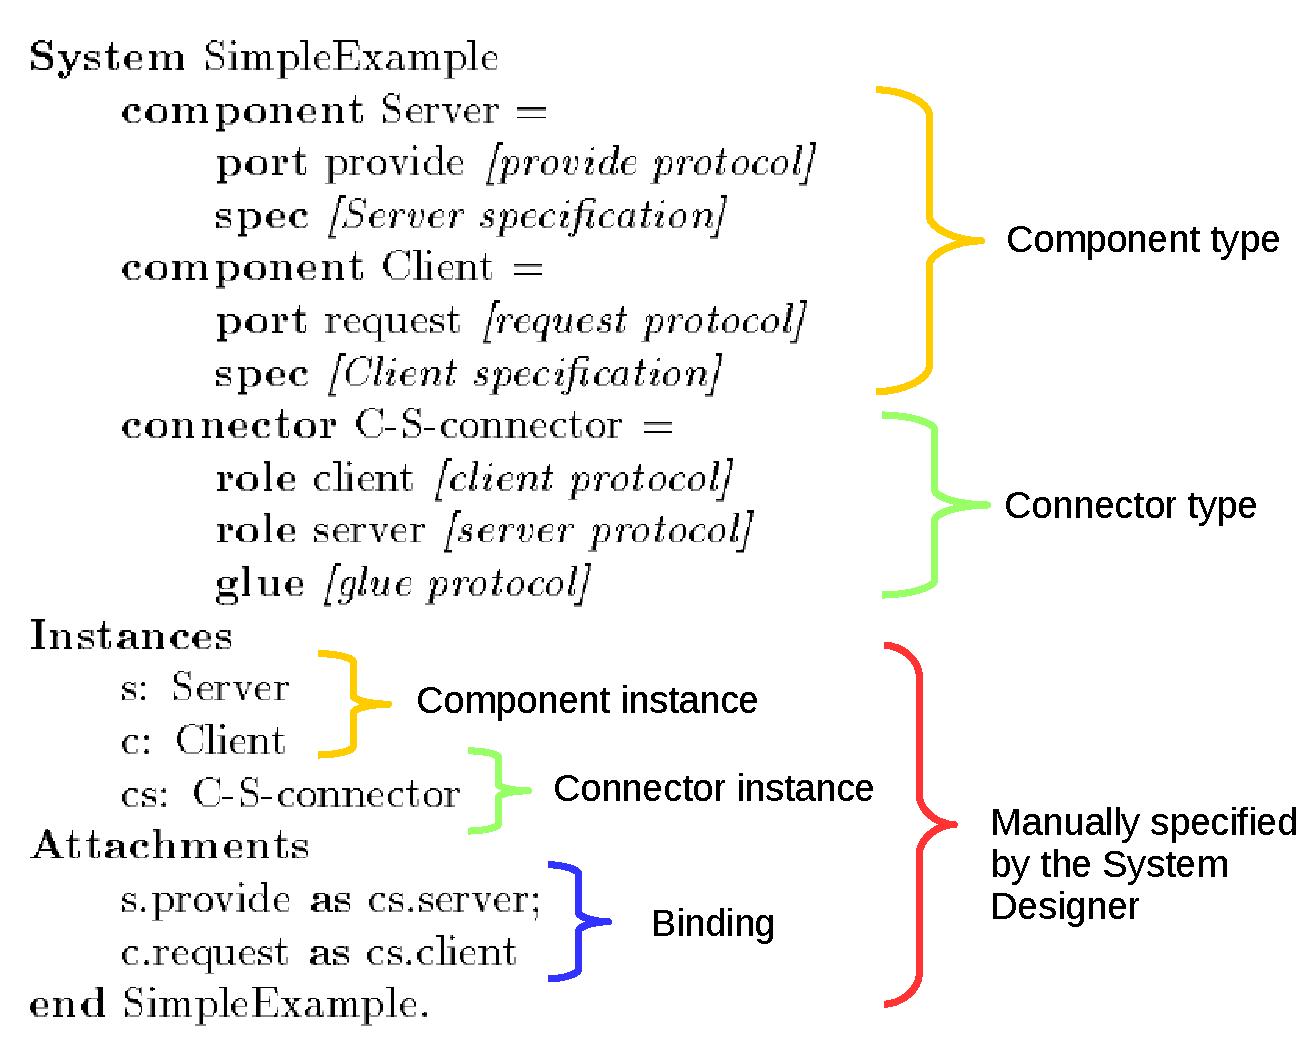
\includegraphics[width=0.5\columnwidth]{background/figs/wrightspec}
					\caption{Specification of a Client-Server system in Wright~\cite{wrightbib}}
					\label{fig:wrightspec}
				\end{center}
			\end{figure}
			
			\item Other approaches introduced a notion of user defined type~\cite{uniconbib,wrightbib,reobib}. These ADLs can then be specialized to a specific domain by the creation of domain specific types. A connector type is usually defined by a set of roles and a glue specification. Roughly speaking, a role represents a formal parameter that is used by the specification of the glue. The glue specification specifies how the activities of the roles are coordinated. This glue can be specified more or less formally depending on the domain need. For instance, in Wright~\cite{wrightbib}, the glue is specified in a variant of CSP~\cite{csphoarebib} while in Reo it is specified by the composition of dedicated primitives~\cite{reobib}. The connector types are later on instantiated and the roles are bound to the actual interfaces of the instances of components. Figure~\ref{fig:wrightspec} shows a simple client-server system described in Wright~\cite{wrightbib}. The specification defines two component types named \emph{Client} and \emph{Server}, and one connector type named \emph{C-S-connector}. The C-S-connector has two roles (\emph{client} and \emph{server}) and a glue that describes how the activities of the client and server roles are coordinated. The section \emph{Instances} describes a particular configuration by instantiating the corresponding components and connectors. The example describes a system where there is a single server (\emph{s}), a single client (\emph{c}) and a single connector (\emph{cs}). Then, the section \emph{Attachments} defines which component ports are attached to the connector roles. This example illustrates how a system designer can define a set of domain specific connector types, and then, instantiate and bind the connector types as needed by its architecture. These connector types are qualified as pattern of interactions in \cite{wrightbib}. 
			
			\item \todo{Following paragraph must be rewritten}
			\item The major drawback of these approaches is that the instantiation and binding of connector types is done manually by the system designer. Returning to the example of Figure~\ref{fig:wrightspec}, for each server and client in the system, the system designer has to instantiate two components and one connector. Then, he has to bind the component ports with the connector roles. With the increasing number and heterogeneity of the components, this task can quickly becomes difficult and error prone. More recent approaches~\cite{dinatale,mascotbib,ptoleframebib,modhelxbib} identified that the instantiation and binding of connector types can be a systematic activity the system designer repeats many times and can consequently be defined as a pattern. Such a pattern is based on the know-how of the system designer and sometimes on naming or organizational conventions adopted by the models. Thus, they have captured the specification of such a behavioral coordination pattern into a tool to automate the instantiation and binding of connector types. They specify the coordination between heterogeneous languages instead of specifying it between particular models (see Figure~\ref{fig:coordpatterapp}). Such specification is then applied on a set of models to automatically instantiate a set of connector types and bind their instances. We refer to these approaches as coordination pattern approaches. In the following section, we overview them by focusing on how a particular coordination pattern is captured by specifying the coordination between a set of heterogeneous languages.
         
         \end{itemize}
         
         \subsection{Coordination Pattern Approaches}
         
         \begin{itemize}
         	\item These approaches automate the coordination of models. There are systematics approaches like Ptolemy~\cite{ptoleframebib} and ModHel'X~\cite{modhelxbib}. Less systematic are MASCOT~\cite{mascotbib} and Di Natale et al.~\cite{dinatale}. These approaches are similar than the coordination is specified between languages but its application is between models.  
         	
         	\item \todo{In this section, we present an overview of the following approaches: Di Natale et al.~\cite{MarcoModels2014}, MASCOT~\cite{mascotbib}, Ptolemy~\cite{ptolemybib}, ModHel'X~\cite{modhelxbib}. These approaches go one step forward than Coordination Languages and ADLs since:
         		\begin{itemize}
         			\item They capture the know-how of a system designer in a certain domain. 
         			\item They specify the coordination between a set of languages by relying on information about theirs syntaxes and semantics. 
         		\end{itemize}	 }
         	
         	\begin{figure}
         		\begin{center}
         			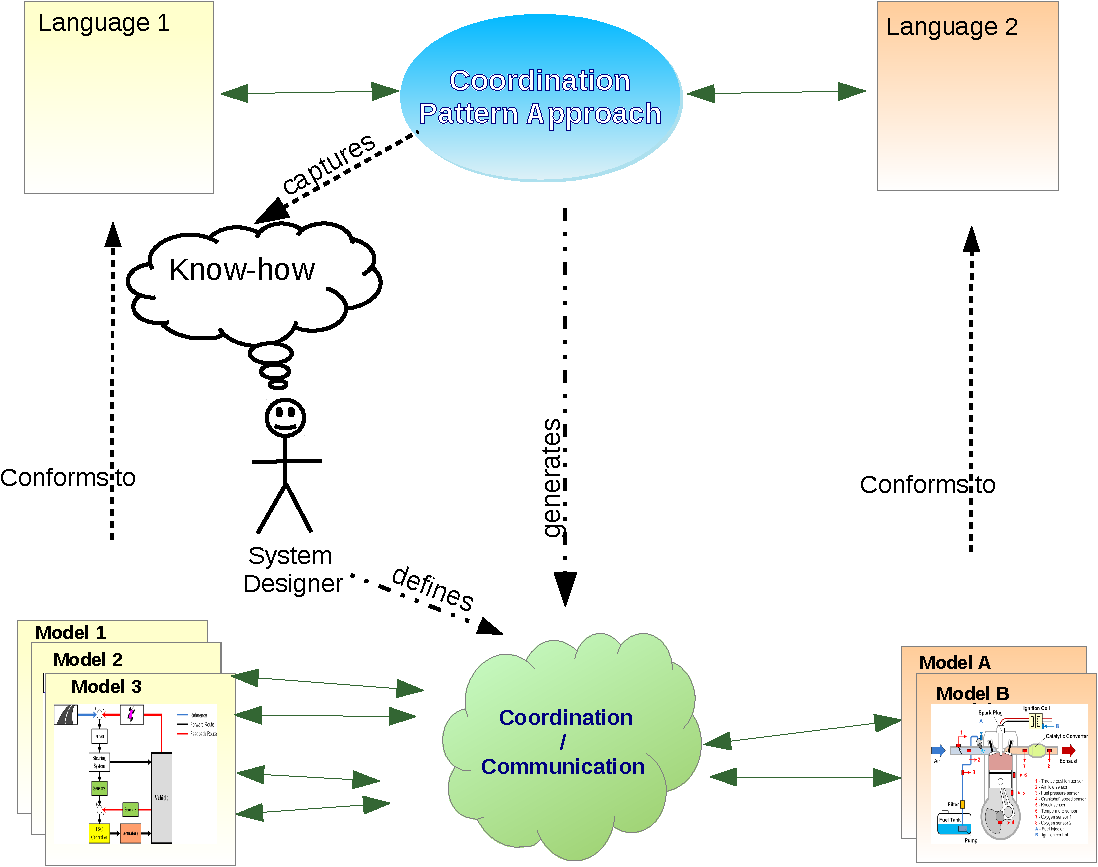
\includegraphics[width=0.6\columnwidth]{framework/figs/coordpatterapp}
         			\caption{Overview of a Coordination Pattern Approach}
         			\label{fig:coordpatterapp}
         		\end{center}
         	\end{figure}
         	
         	\begin{figure}
         		\begin{center}
         			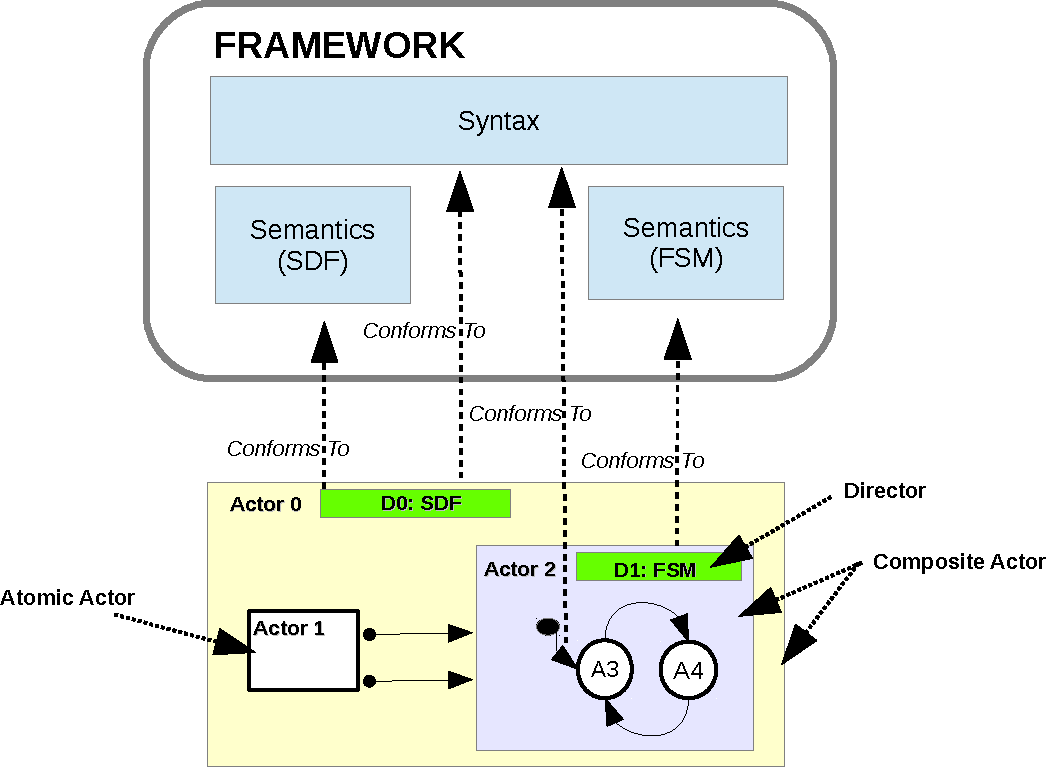
\includegraphics[width=0.7\textwidth]{background/figs/ptolemyfig}
         			\caption{High level view of Ptolemy~\cite{giraultbib}}
         			\label{fig:ptolemyfig}
         		\end{center}
         	\end{figure}
         	
         	\item Ptolemy~\cite{ptoleframebib} and ModHel'X~\cite{modhelxbib} are coordination frameworks that rely on a common syntax based on actors and a semantics given by Models of Computation (MoC). These approaches represent models as actors that can be atomic (\eg \emph{Actor 1} in Figure~\ref{fig:ptolemyfig}) or composite (\eg \emph{Actor 0} and \emph{Actor 2} in Figure~\ref{fig:ptolemyfig}), \ie made of internal actors. Each composite actor has associated a model of computation implemented as a \emph{Domain}. A domain defines the communication semantics and the execution order among internal actors. A domain is implemented by a \emph{Director}. For instance, in Figure~\ref{fig:ptolemyfig}, the \emph{Actor 0} has the director \emph{D0} that follows the semantics of SDF and the \emph{Actor 2} has the director \emph{D1} that follows the semantics of FSM. In this approach, actors, both atomic and composite, are executable. In a composite actor, the execution order of internal actors is controlled by a director. In the example of Figure~\ref{fig:ptolemyfig}, the director \emph{D0} controls the execution of the \emph{Actor 1} and \emph{Actor 2} and director \emph{D1} controls the execution of \emph{A3} and \emph{A4} whenever \emph{Actor 2} is executed. In this sense, the execution of composite actors is strictly hierarchical. The behavior of actors is represented by a generic interface that contains a set of methods, \eg fire(). The MoC implemented by the director of a composite actor specifies when the methods in the interface of internal actors are invoked. For instance, when a composite actor is fired, the director associated with the composite actor fires the actors of the contained model. Based on a fixed syntax and a generic interface, these approaches have achieved to capture a hierarchical coordination pattern into a framework. The framework provides a dedicated syntax to specified the pattern, \ie composite actors, and encodes the necessary glue between interfaces to coordinate their execution. 
         	
         	
         	
         	\begin{figure}
         		\begin{center}
         			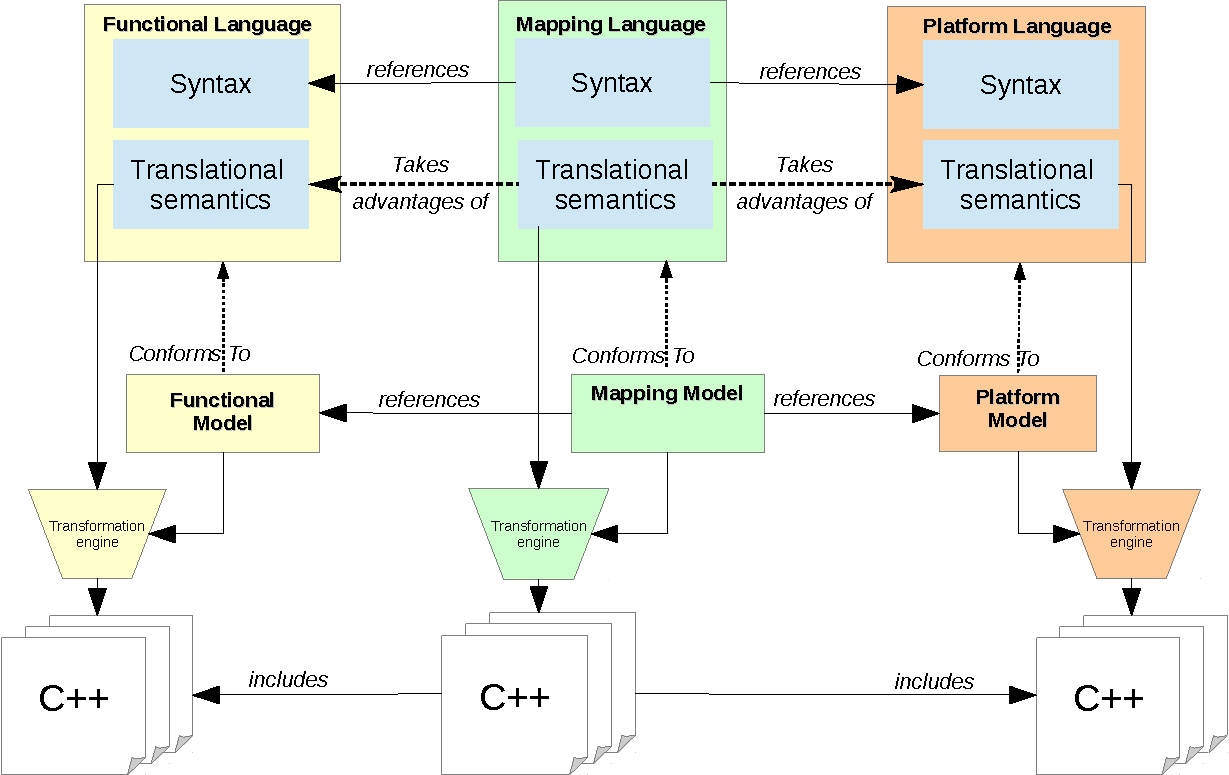
\includegraphics[width=0.7\textwidth]{background/figs/diNatale}
         			\caption{High Level view of the approach proposed by Di Natale et al. in~\cite{dinatale}}
         			\label{fig:diNatale}
         		\end{center}
         	\end{figure}
         	
         	
         	\item MASCOT~\cite{mascotbib} is a different approach focused on the integration of Matlab~\cite{matlabbib} and SDL~\cite{sdlbib}. Whereas SDL is a language suitable for control systems modeling, Matlab is better for modeling dataflow aspects of a system. However, these languages are very different, while SDL processes operate on events, represented by simple signals, Matlab processes operate on vectors, represented by vectorized signals. Thus, authors propose to automate the synchronization of control signals from SDL with data signals from Matlab. These signals can be either notification signals or message signals. Notification signals do not carry a value and are used to notify a process that an event has occurred. Message signals carry a value and are used to indicate a change of some variable or parameter. The approach deals with the integration of the timing and synchronization concepts from both languages by proposing two synchronization modes: head synchronization and tail synchronization. These mechanisms take advantages of the knowledge about the semantics of the languages. For instance, in the head synchronization, when a model in matlab receives a frame \emph{a1}, it immediately transforms \emph{a1} into \emph{b1} (dataflow network model). Any control signal from SDL that occurs during the transformation of \emph{a1} to \emph{b1} cannot influence its value. Then, the head synchronization mode ensures that the occurrence of the control signal is taken into account when the next frame is processed. In the tail synchronization, when a model in Matlab receives a control signal from SDL, the signal is collected until it cease to occur, then, it is translated to a vector and passed to the Matlab model. The modes of synchronization ensure the communication between Matlab and SDL. In addition, the approach gives a set of guidelines to aid the system designer to choose between the two synchronization proposed. Once the synchronization policy is defined, the approach enables the co-simulation of a SDL model and a Matlab model. The implementation is based on SDL wrappers. A process in the SDL specification that is specified in Matlab contains a wrapper that interfaces between the SDL simulator and the Matlab engine. A SDL wrapper is made of a set methods that enable the SDL engine to control the behavior of the data signals in Matlab. To do so, the approach relies on the name of signals in SDL specification to communicate with the signals in Matlab. The approach thus forces the system designer to follow a naming convention between signals in both domains. The current implementation partially automates the coordination of signals from both domains. However, the approach has identified and captured a coordination pattern between a control-flow language and a data-flow language by relying on some knowledge about its syntax and semantics.
         	
         	\item In~\cite{dinatale}, authors propose a dedicated language to map a functional model to a platform model (see Figure \ref{fig:diNatale}). Both the functional and the platform syntaxes were equipped with a translational semantics to C++ code. Then, based on the mapping model, the approach generates the code of the communication connectors between the code obtained from the functional and platform models. A first interesting aspect of this approach comes from the possibility, by creating a dedicated language, to reuse existing languages, and based on a mapping model to automatically generate the glue between the implementation of the models (in this case encoded in C++). By having a closer look at the approach, the mapping language syntax references syntactic elements from both the functional and the platform language. For instance, the $SWdeployment$ concept from the mapping model, reference the $Task$ concept from the functional model and the $CPU$ concept from the platform model. Also, the translational semantics of the mapping language takes advantages of some knowledges about the translational semantics of the other languages. For instance, for each subsystem, authors know that a class is generated with name \emph{SubsystemName}\texttt{ModelClass}. They also know that the class has a \texttt{step} operation for the runtime evaluation of the block outputs given the inputs and the state. In other words, authors have a partial but sufficient knowledge of the translational semantics of both the functional and the platform language. Finally, based on this knowledge, they encode in the translational semantics the glue to generate according to the actual mapping in the mapping model. The approach proposes a set of connectors that the system designer has to instantiate in the mapping model. In this sense, the approach is similar than the ADLs Clara, which proposes a set of built-in connectors. However, different than other ADLs, the approach proposes connectors that link concepts from different languages. In particular, these connectors capture some knowledge of a system designer that performs the mapping of a functional model to a platform model.
         	
         	
         \end{itemize}
         
\subsection{Discussion}
\begin{itemize}
	\item \todo{We need a coordination at the language level, explicit by using a dedicated language and that enables the verification and validation of the coordinated system}
	\item To capture once and for all the know-how of the integrator, some approaches capture coordination patterns by specifying the coordination at the language level. This is the case for coordination frameworks like Ptolemy and ModHel'X, which rely on hierarchical coordination patterns between heterogeneous languages. This is also the case for solutions like MASCOT~\cite{mascotbib}, which provide ad-hoc coordination patterns (\ie between Matlab and SDL). Once the coordination pattern between a set of languages is captured, the models conforming to such languages can be coordinated automatically. Such approaches successfully capture the know-how of the integrator, however, they do so by embedding the coordination pattern inside a tool. As a result, the integrator cannot change the coordination specification without altering the core of the tool. However, for complex systems, the integrator may need to capture several coordination patterns and potentially combine them. This is highlighted in~\cite{giraultcompo} where authors use Ptolemy to capture three hierarchical coordination patterns between a finite state machine with Data flows, a Discrete event model and a Synchronous/Reactive model. Since each coordination pattern is applicable in different situations, authors argue that each one is useful. Thus, the integrator must be able to capture different coordination patterns since there is not necessarily a single \emph{valid} one. However, current coordination frameworks can only support such a variation by modifying the framework itself. Additionally, the coordination model is mixed with the functional model, which makes it very tricky to modify one without risking altering the other.
	
	\item During the integration activity, the integrator must be able to capture different coordination patterns and their semantics must be explicit rather than being hidden inside a tool. To illustrate this, Gabor et al.~\cite{gaborpolyglot} show the semantic variations of Statecharts presented in different tools. Since each approach interprets differently the semantics of Statecharts, we obtain different behaviors depending on the approach. However, if the semantics is hidden inside the tool and is not made explicit, this can lead to misunderstandings and errors. Moreover, validation and verification activities are limited in current coordination frameworks since the coordination is encoded by using a general purpose language.
	
	\item \todo{The knowledge about system integration is currently either implicitly held by the integrator or encoded within a framework. To capture explicitly this knowledge and thus leverage integrator know-how, we propose a dedicated language to capture coordination patterns between languages, thus reifying the coordination specification at the language level.}
	
\end{itemize}

\section{Conclusion}
In this chapter, we have presented a background of current approaches that deal with the integration of heterogeneous models and languages. 

We have presented approaches that compose heterogeneous models/languages in order to obtain a new model/language. The composition of models has been automated by looking for correspondences between heterogeneous model, and then composing them into a new model that can conform to other language. 
While most of the approaches only consider structural correspondences, only a few consider also the behavior of model to find similarities. Furthermore, we have determined that these approaches only compose homogeneous models. This limits the use of such approaches in complex systems where heterogeneous behavioral models may be used.

Unlike the composition of models, we have noted that the composition of languages has not been automatized. Thus, a system designer has to 1) find correspondences between concepts of different languages and 2) specify how these concepts are related. This results in a new language. The inputs languages and the composed language are conformed to the same meta metamodel. In most of these approaches, the correspondence are only between syntactic elements, and only one approach enables to define behavioral correspondences in order to obtain a new behavioral semantics.  

We want to highlight that an specification at language level (as proposed by composition models approaches) is easier to handle than a unified language (as proposed by composition of languages Approaches). From our point of view, Composition of Languages approaches are not suitable for separation of preoccupation and development of a single system by various domain experts that focus on a specific part of the system.

Afterwards, we have presented the state of art approaches that deal with coordination of the behavior of heterogeneous models/languages. First, we have presented the work done by Coordination Languages and ADLs that support the coordination of heterogeneous models. However, the system designer has to manually specify each relation, thus making this task tedious and error prone. Then, we have shown how coordination pattern approaches have leveraged on the know-how of system designer to automate the coordination between models. However, we have noted that the knowledge about system integration is encoded within a framework. Furthermore, in frameworks, the model of coordination is expressed by using a general purpose language thus limiting verification and validation activities. 

%We want to highligne that the current integration of languages is based on two mechanism: composition and coordination. While composition tends to provide to compose language into a new language, Coordination tends to provide a model of coordination which is external to the models itself. It is interesting that coordination only considers behavioral while composition only structural. Why? 
In this thesis, we propose to capture explicitly the know-how of a system designer by using \bcool, a dedicated language to capture coordination patterns between languages, thus reifying coordination at the language level (see Figure~\ref{fig:bcoolapp}). From this specification, a formal model of coordination is generated. This enables validation and verification of the coordinated system. 

In the next chapter, we focus on coordination pattern approaches to understand how a given coordination pattern is being captured. We leverage on such knowledge to built \bcool. 

\begin{figure}
\begin{center}
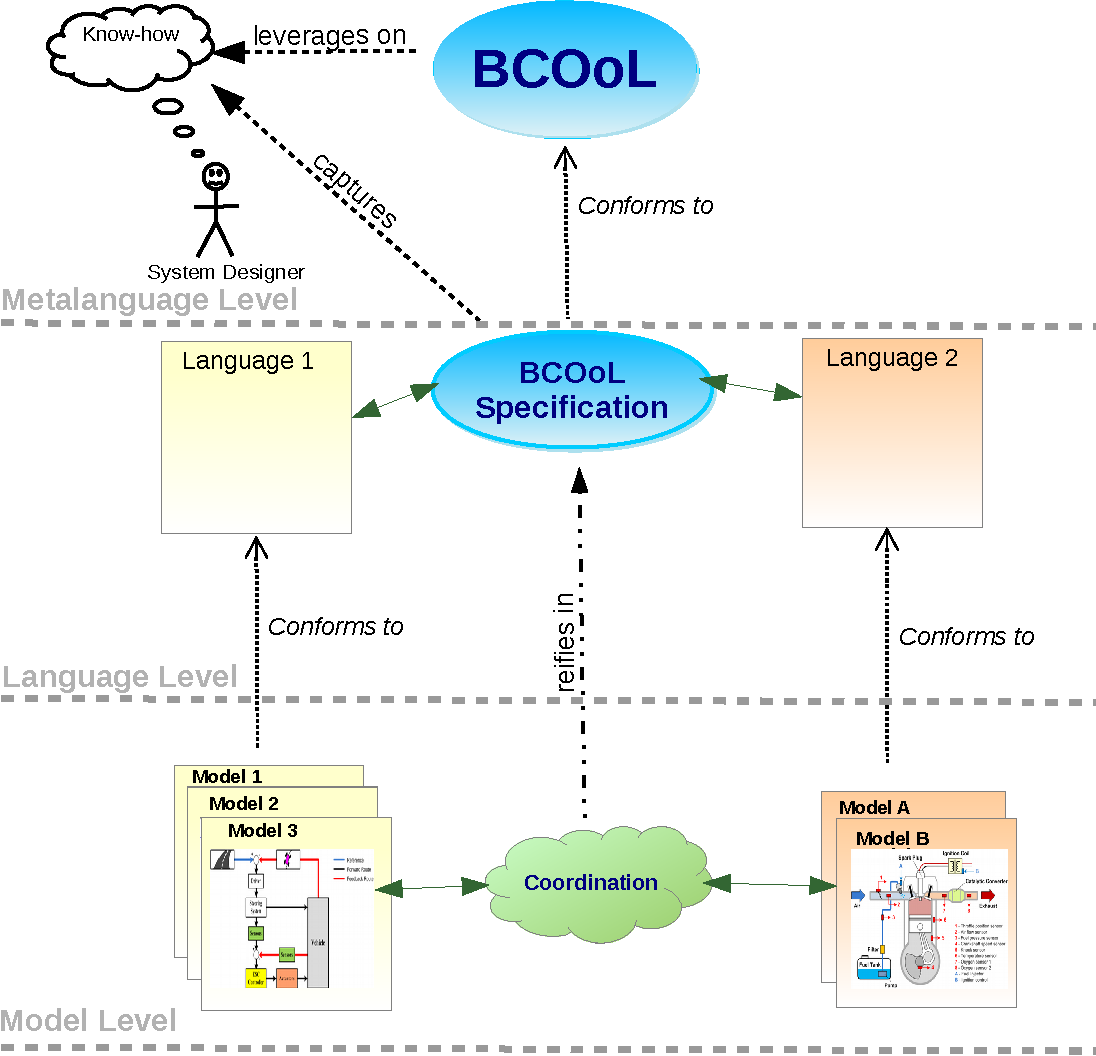
\includegraphics[width=0.7\textwidth]{background/figs/bcoolapp}
\caption{Overview of Our Approach}
\label{fig:bcoolapp}
\end{center}
\end{figure}	


%\begin{landscape}% Landscape page
%\begin{table}[]
	%\centering
	%\caption{Overview of Behavioral Composition/Coordination Approaches}
	%\label{tbl:overview}
	%\resizebox{\textwidth}{!}{%
		%\begin{tabular}{@{}|c|l|l|c|c|c|c|c|c|c|
			%	>{\columncolor[HTML]{9AFF99}}c |@{}}
			%\toprule
			%\multicolumn{3}{|c|}{} & \multicolumn{2}{c|}{Behavioral Composition Approaches} & \multicolumn{3}{c|}{Coordination %of Model Approaches} & \multicolumn{2}{c|}{Coordination Pattern Approaches} & Our Approach \\ \cmidrule(l){4-11} 
			%\multicolumn{3}{|c|}{\multirow{-2}{*}{}} & Semantic Anchoring & \cite{compostatechartsbib} & Esper & Rapide & BIP & %Ptolemy & Di Natale et. al & BCOoL \\ \midrule
			%\multicolumn{3}{|c|}{Number of Languages/Models Supported} & 1 & 1 & N & N & 1 & Predefined set & 2 & N Languages %\\ \midrule
			%\multicolumn{3}{|c|}{Specification of the Coordination (from a system designer point of view)} &  & Implicit & %Explicit & Explicit & Explicit & Implicit & Impicit & Explicit \\ \midrule
			%\multicolumn{3}{|c|}{Glue (coordination at model level)} &  &  & Formal & Formal & Formal & Java (generated) & C++ %(generated) & Formal (generated) \\ \bottomrule
%		\end{tabular}
%	}
%\end{table}
%\end{landscape}

\chapter{Framework for Coordination Pattern Specification}
\label{ch:framework}

\section{Introduction}
\todo{This INTRO has to be REDO!}
\begin{itemize}
\item In this chapter, we present a deep study on coordination pattern approaches. 

\item These approaches are implemented by using different technologies. However, they can be seen as different implementations (sometimes partial) of a same conceptual framework.

\item The conceptual framework we propose comes from a deep understanding of the different approaches and the internal mechanisms they used. We tried to abstract these mechanisms to extract the essence of the information needed to specify a behavioral coordination pattern between heterogeneous languages. The conceptual framework can be used to better understand the existing approaches but also to define requirements about a more general and systematic way to define such approach.


\item We are inspired by the framework presented in~\cite{framecompoas} to compare model
composition techniques. The framework relies on the triplet \emph{what?}, \emph{where?} and \emph{how?} questions that identify respectively which elements should be composed, where elements should be inserted or modified and how the composition process works to get the expected result. 


\item By relying on this work, we propose a framework for coordination pattern approaches. The goal of this framework is to characterize the mechanisms involved into the coordination pattern approaches. We rely on three questions: \emph{What?}, \emph{When?} and \emph{How?} that identify what concepts can be coordinated, when such elements must be coordination and how the selected elements must be coordinated.   
 

\item In the following, we present these elements.     
	
\end{itemize}


\section{Language Behavioral Interface}
	\subsection{Overview}
	\begin{itemize}
		\item The language behavioral interface provides \emph{What?} can be coordinated. A language behavioral interface is a partial representation of the behavioral semantics and syntax of a language. The behavioral interface contains the needed information to coordinate the behavioral of languages. 
		\item In Coordination Languages and ADL, there exists a notion of model behavioral interface. Such interface expose the needed information to ease the coordination of models. The content of the interface varies from one approach to other. However, the main goal is to ease the task of a system designer in order to ease the coordination of models.  
		\item In the case of Coordination Pattern approaches, we identified that approaches base on some knowledge on the semantics and syntax that they compose. Such knowledge is partial. We name this language behavioral interface. 
		\item The concept of language behavioral interface is not presented in the structural framework. 
		\item In the following, we present this concept in relation with the studied approaches. However, such a concept is not always identified as an interface by the approaches.   
	\end{itemize}

	\subsection{Comparison}
		\begin{itemize}
		
			\item In Ptolemy~\cite{ptolemybib} and ModHel'X~\cite{modhelxbib}, models conform to the same abstract syntax based on the actors. The behavioral semantics depends on the Director that implements a Model of Computation. A director encodes the behavioral semantics in Java. Then, to communicate different Directors, the approach is based on a notion of generic language behavioral interface. In this case, the interface is made of methods in Java. The approach forces the prototype of the functions to encode a given model of computation. The approach specifies the semantics of the method in natural language. For instance, a part of the \emph{fire()} function description is: ``\emph{Typically, the fire() method performs the computation associated with an actor}''. It can also be noticed that the name of the director usually brings some semantics to the people aware of Model of Computation and can be considered as part of the language interface. However, using the director name remains very informal. A generic interface enables to provide an homogenous view of the behavioral semantics of different languages. Then, the pattern is captured by specifying how the method from different interfaces are invoked. 
			
			%\item In Ptolemy~\cite{ptolemybib} and ModHel'X~\cite{modhelxbib}, the coordinated models are all conforming a unique abstract syntax but with different behavioral semantics. Both approaches are based on the notion of \emph{Director}, which encodes the behavioral semantics in Java. A \emph{Director} implements a specific Java interface\footnote{the Executable interface, cf.} %\url{http://chess.eecs.berkeley.edu/ptexternal/src/ptII/doc/codeDoc/ptolemy/actor/Executable.html}}, which provides an homogeneous view of the behavioral semantics of a language by enforcing the prototype of the functions used to encode the semantics. The semantics behind the methods are given in a natural language. For instance, a part of the \emph{fire()} function description is: ``\emph{Typically, the fire() method performs the computation associated with an actor}''. The function prototypes, together with their informal description provides an homogeneous view of the semantics of the languages, which is used to specify the coordination pattern. It can also be noticed that the name of the director usually brings some semantics to the people aware of Model of Computation and can be considered as part of the language interface. However, using the director name remains very informal.
			
			\item In~\cite{dinatale}, the mapping language only has partial information about the syntax of both the functional and the platform languages. The mapping language references only some of the syntactic elements from both languages (\eg \emph{Task}s and \emph{Cpu}s). In addition, the translational semantics of the mapping language is based on the knowledge about the translational semantics of the platform and functional languages. More precisely the mapping semantics needs to know about the naming conventions from the other translational semantics. In~\cite{dinatale}, this required knowledge is kept implicit and hard coded in the translation semantics of the mapping language. However, this information about the language semantics could be exposed in a language interface to avoid hard coding it. 
			
			\item In Mascot~\cite{mascotbib}, the coordination is not symmetric since Matlab scripts are embedded in an SDL model. \todo{As a consequence the Matlab interface is used but not the SDL interface.} The authors identified two main elements about the Matlab language. First they depict the different kinds of communication used from and to Matlab. Second they characterize the Model of Computation used by the Matlab simulation engine as being Petri Net. They based the coordination on this knowledge so that these pieces of information act as the language interface of the Matlab language. \todo{On the other side, it is mandatory in the Matlab script to use the same name for the stream then the name of the signals from and to the SDL wrappers of the SDL model. Consequently, it means this approach relies on naming convention to specify the correspondence matching.}
		\end{itemize}
	\subsection{Discussion}
	\begin{itemize}
	
	    	\item All the approaches studied retrieve information on the syntax and/or behavioral semantics of the languages they coordinate. Only \cite{ptolemybib} and \cite{modhelxbib} made explicit the notion of interface; \cite{MarcoModels2014} and \cite{mascotbib} retrieved the information implicitly from the definition of the languages. 
	    	Using an explicit language interface is a way to obtain a language independent representation of the behavioral semantics. In this case, the approaches can add support to new languages with a minimum effort since they are seen homogeneously. However, because the language interface definition used in \cite{ptolemybib} and \cite{modhelxbib} provides only a list of functions, it requires a deep understanding of the underlying framework to be able to specify correct coordination patterns. 
	    	\todo{An interesting research direction could be to adapt the notion of interface automata proposed in~\cite{henzingerIA} to specify the acceptable protocol between the calls of the functions that implements the semantics of the language.} 
	    	
	    	\item At the model level, \cite{garlansoftarchbib} explains that there are important benefits of using events (with implicit invocation) in the component interfaces because it provides strong support for reuse and evolution of components. 
	    	In~\cite{coordinainterfacebib}, authors go further by proposing a component interface that contains events but also properties specified in a temporal logic language. These properties abstract the behavior of the components.
	    	
	    	\item \todo{Some coordination languages deal with the complexity of model behaviors by treating models as black boxes encapsulated within the boundary of an interface. A model behavioral interface gives a partial representation of the model behavior therefore easing the coordination of behavioral models. However, it is not uniquely defined and may vary depending on approaches. For instance, in \emph{Opus}~\cite{Opus}, the interface is a list of methods provided by the model. Other approaches abstract away the non-relevant parts of the behavior of models as events~\cite{eventStructures} (also named signals in~\cite{lee1998framework}). These approaches focus on events and how they are related to each other through causal, timed or synchronization relationships. Following the same idea, \emph{control-driven} coordination languages rely on a model behavioral interface made of explicit events~\cite{rapide,esperbib,coordinainterfacebib}. While in Rapide~\cite{rapide}, the interface is only a set of events acceptable by the model, some other approaches go further and also exhibit a part of the internal concurrency. This is the case of~\cite{coordinainterfacebib} where authors propose an interface that contains services and events, but also properties that express requirements on the behavior of the components. Such requirements act as a contract and can be checked during the coordination to ensure a correct behavior. In these approaches, the model behavioral interface provides information to coordinate the behavior of a model. In particular, in event-driven coordination approaches events act as ``coordination points" and exhibit what can be coordinated. This gives a support for control and timed coordination while remaining independent of the internal model implementation. Moreover, event-driven coordinations are non intrusive; \ie models can be coordinated without any change to their implementation, thus ensuring a complete separation between the coordination and the computational concerns. Several causal representations from the concurrency theory are used to capture event-based behavioral interface. A causal representation captures the concurrency, dependency and conflict relationships among actions in a particular program. For instance, an event structure~\cite{eventStructures} is a partial order of events, which specifies the, possibly timed, causality relations as well as conflict relations (\ie exclusion relations) between actions of a concurrent system. This fundamental model is powerful because it totally abstracts data and program structure to focus on the partial ordering of actions. It specifies, \emph{in extension} and \emph{in order}, the set of actions that can be observed during the program execution. An event structure can also be specified \emph{in intention} to represent the set of observable event structures during an execution (see \eg\cite{tr:ccsl} or \cite{tagmachine}).}
	    	
	    	\item With the goal to provide a rich event based language interface, \cite{sle13combemalebib} proposed to specify a behavioral language interface based on the notion of symbolic event structure. The symbolic event structure is linked to both the abstract syntax and the functions implementing the semantics. It exhibits the concurrency and the causalities between the functions implementing the semantics and link them with the concepts of the language.
	    	
	    	\item \todo{In~\cite{sle13-combemale} elements of event structures are reified at the language level to propose a behavioral interface based on sets of \emph{event types} and \emph{contraints}. Event types (named \dse for Domain Specific Event) are defined in the context of a metaclass of the abstract syntax (\as), and abstract the relevant semantic actions. Jointly with the \dse, related constraints give a symbolic (intentional) representation of an event structure. With  such an interface, the concurrency and time-related aspects of the language behavioral semantics are explicitly exposed and the coordination is event-driven and non intrusive.}
	    	\item \todo{Then, for each model conforming to the language, the model behavioral interface is a specification, in intention, of an event structure whose events (named \mse for Model Specific Event) are instances of the \dse defined in the language interface. While \dse are attached to a metaclass, \mse are linked to one of its instances. The causality and conflict relations of the event structure are a model-specific unfolding of the constraints specified in the language behavioral interface. Just like event structures were initially introduced to unfold the execution of Petri nets, we use them here to unfold the execution of models.}
	    	\end{itemize}

\section{Correspondence Rules}
This section presents the notion of \emph{Correspondence Rules}. We first review the concept of correspondence rules in existing approaches, and then, we present requirements to make them explicit and better customizable.  

\subsection{Review of Existing Approaches}
A correspondence is any explicit or implicit relationship between model elements. Such a relationship is specified by a system designer that knows what elements from different models are related. In the specification of coordination patterns, correspondences specify the model elements that are coordinated. To automate the process of looking for correspondences between models, the specification of a coordination pattern involves the definition of correspondence rules at language level. Such rule define, in intention, the correspondences to be instantiated at model level. In the following, we review the existing approaches by focusing on how they implemented correspondence rules and correspondences.       
%A correspondence rule is a specification in intention, at the language level, of the correspondences to be created at the model level. In the following we review how the different approaches deal with correspondences and correspondence rules.

\paragraph{Ptolemy~\cite{ptoleframebib}/ModHel'X~\cite{modhelxbib}:}
In these approaches, the notion of composite actors is used to specified the correspondences between models: when an actor is composite (\ie it contains other actors) then it coordinates its internal actors. This enables the designing of a system by following a hierarchical scheme where the level $n$ in the hierarchy specifies the coordination of the models that are at the level $n-1$. These approaches propose a fixed correspondence rule, \ie the composite actor relation, which is encoded into the syntax of the framework.

The \emph{pro} of these approaches is the simplicity for a designer to express the correspondences. He has only to specify what models are composited and which ones are contained inside. The correspondence rule is unique and provided into the common abstract syntax. 

The main \emph{cons} of these approaches is they rely on a unique abstract syntax to describe both the syntax of models and the syntax of the correspondences. This prevents the independent development of the models (possibly developed in different languages) and the correspondences. In addition, the use of a hierarchical design may limit the number of the supported languages. For instance, the UML sequence diagram could not be easy to introduce in the hierarchical view of the framework.

\paragraph{Di Natale et al.~\cite{dinatale}:}
In this work, a mapping model is used to define the correspondences between the functional and the platform model. The mapping model is defined by using a dedicated language (\ie mapping language) that fixes what type of concepts between the platform and the functional languages can be bound together. For instance, the \emph{SwDeployment} correspondence maps two types of concepts: one of type \emph{CPU} and another one of type \emph{Task}. In this sense, the approach provides a set of fixed correspondence rules. 

The \emph{pro} of the approach is that the mapping model defines explicitly the correspondences between the functional and the platform model. Such a model could be useful both reasoning and for traceability. 

The \emph{cons} of this approach is that a system designer has to manually build the mapping model depending on the current deployment. The approach has successfully identified some relationships between a functional and a platform language, which are captured by a set of predefined correspondence rules. From such a correspondence rules, the approach, however, is not able to automate the instantiation of correspondences at model level. 

{\paragraph{Mascot~\cite{mascotbib}:} In this work, the correspondences are implicit in the models. The approach relies on a naming convention to specify when events in SDL and streams in Matlab must be coordinated. It relies on a correspondence rule that specifies that the elements to be coordinated must have the same name. When this rule is applied between models, the framework can automatically get correspondences between model elements.

The \emph{pro} of this approach is the use of a correspondence rule to select model elements. This makes the approach very flexible in terms of dependencies between the languages, thus easing the support for a new language.  

The \emph{cons} is the encoding of the correspondence rule in the framework. Thus, the approach is limited to find correspondences by comparing the name of the elements (\ie events from SDL and streams from Matlab). In some cases, it could be interesting to compare more than the names, \eg the types. In addition, the approach forces the use of a naming convention in the models.     


\subsection{Requirements}
In the reviewed approaches, we identified different correspondence rules to get correspondences between models elements. Ptolemy and ModHel'X rely on a common abstract syntax to identify the elements to be coordinated; Di Natale et al. propose a dedicated language to express an explicit mapping between the elements of different models; and Mascot defines some rules that allow the inference of the correspondences for specific models. However, the main drawback of these approaches is that the customization of the correspondence rules is not possible. Such a characteristic motivates the following requirements for correspondence rules and correspondences:

\begin{enumerate}
	\item Correspondence rules should provide support for heterogeneous languages; 
	\item Correspondence rules should avoid creating dependencies between a predefined set of languages to enable the support of new languages;
	\item Correspondence rules must be explicitly defined and customizable depending on the domain and conventions followed by different system engineers;
	\item Correspondences between model elements should be explicitly represented.  
\end{enumerate}

We discuss each requirement in turn. The current development of complex systems is tackled by relying on several heterogeneous languages where each language has its own syntax and behavioral semantics. Thus, an approach that capture the specification of a coordination pattern must be able to identify correspondences between models that are heterogeneous in terms of the syntax. This prevents the possibility to rely on a common syntax for the languages and the correspondences like in Ptolemy and ModHel'X.


The support of heterogeneous languages should be done in a way that a new language can be easy to add. For instance, in the case of Di Natale et al., the mapping language (\ie the language used for the correspondences) depends on the coordinated languages, (\ie the functional and the platform languages). So that, if any of these languages are modified or a new language has to be added, the mapping language must be changed. Instead, correspondence rules could be defined by relying on partial information exposed in the interface. This would avoid strong dependencies between the correspondence rules and the coordinated languages.

%We believe that the correct specification and use of a homogeneous language interface could also act positively towards this requirement. 

%The first important requirement to face the globalization of modeling languages is the support for heterogeneous languages, not only in terms of semantics but also in terms of syntax. 

%Such support disable the possibility to rely on an artifact of a common abstract syntax like in Ptolemy and ModHel'X. However, it paves the road of an open world with emerging (domain specific) languages as depicted in~\cite{globalization_ieee}.

%Also, in order to address correspondences while taking into account the globalization of modeling languages, it is important to avoid the creation of strong dependencies when specifying the correspondences and the correspondence rules. 

%While this requirements ease the support of new languages, it makes difficult to strongly type or constraint the correspondences. For instance, in \cite{dinatale} the mapping language constrains the mapping model to relate only some specific elements (creating a mapping language with dependencies to the related languages). We believe that the correct specification and use of an homogeneous language interface could also act positively towards this requirement. 

%In Mascot, authors identified that by relying on correspondence rules the process for looking for similarities between models elements can be easily automatized. %These rules are specified at language level and enable to get correspondences between two particular models. However, in MASCOT, these rules are encoded and not well defined. %To improve the definition of correspondence rules, our fourth requirement is that correspondences rules must be explicitly defined and customizable depending on the domain and conventions followed by different system engineers.
A correspondence rule can be used to find correspondences between models that conform to two particular languages. This is the case in~\cite{kofmanbib} where authors use design space exploration techniques to determine the (best) correspondences between an application and its deployment platform. Also, correspondence rules can be used to capture conventions followed by system engineers in an organization. The complexity of the conventions can vary from a simple naming convention (\eg Mascot) to a more complex ontology based system. Based on such conventions, correspondence rules can determine what elements from different models must be coordinated.    

\begin{lstlisting}[language=epsilon, caption={Specification of the Mascot correspondence rule by using the Epsilon Comparison Language}, label={lst:epsilon}, 	basicstyle=\scriptsize\ttfamily, backgroundcolor=\color{LGrey}, numbers=left, xleftmargin=2pt]
rule MatchEventWithStream
match s : SDLMetamodel!Event
with t : MatlabMetamodel!Stream 
{
compare {
	 return s.name = t.name;
	}
}
\end{lstlisting}

To make correspondence rules explicit, a dedicated language should be used. To illustrate this, we propose to use the Epsilon Comparison Language (ECL~\cite{epsilonbib}) to sketch the definition of the correspondence rule in the case of Mascot. The ECL is a language dedicated to the expression of correspondence rules. In this language, correspondence rules are expressed by querying and then comparing model elements. For example, Listing~\ref{lst:epsilon} shows the specification in ECL of a matching rule named \emph{MatchEventWithStream}. Roughly speaking, the matching rule is used to find correspondences between instances of the \emph{Event} and \emph{Stream} classes (Listing~\ref{lst:epsilon}: line 2 and 3). These classes can be defined in different metamodels (\ie Ecore models). The class Event is defined in an metamodel referred as \emph{SDLMetamodel} and the class Stream is defined in an metamodel referred as \emph{MatlabMetamodel} (Listing~\ref{lst:epsilon}: line 2 and 3). The comparison is done by using the attribute name defined in the context of each class (Listing~\ref{lst:epsilon}: line 5). To express the comparison, the approach relies on a query language named Epsilon Object Language\footnote{http://www.eclipse.org/epsilon/doc/eol/}. When two instances of these classes have the same name, the pairs are matched.

The main benefit of the use of such a dedicated language is to ease the customization of the correspondence rules, thus enabling to adapt them according to the company modeling conventions and the language's nature. For instance in Listing~\ref{lst:epsilon}, the matching is equivalent to the one encoded in Mascot, however, it can be customized to add another criteria for the matching. Furthermore, conventions are independent of the languages themselves, so it is easy to add support for a new language without changing the framework.


Finally, to understand how a particular system is coordinated, correspondences between model elements must be clearly represented. This has already identified in the Ptolemy and ModHel'X by providing a dedicated syntax to specify the correspondences. Unlike these approaches, in Mascot, the correspondences are implicit into the approach thus making necessary to read the documentation to find out that the approach relies on a correspondence rule that follows a naming convention. In such a case, an explicit representation of the correspondences can help a system designer to understand the coordinated elements. Also, it allows external tools to take advantages of the correspondences. The explicit representation of correspondences should be done without creating dependencies between the languages used in the system in order to fulfill the second requirement.% \todo{To fulfill this requirement, interfaces (both at language and model level) could be helpful.}
	
	%\item When a system designer tries to understand the correspondence that exists in a coordinated system, it is very useful for her/him to have an explicit representation of these correspondences.
	
	%\item  It avoids ambiguities in the understanding of the coordination but also it allows external tools to take benefits of the correspondences.
	
	%\item This is for instance not the case in the Mascot approach where the correspondences are never reified and only known by the framework and the people aware of the correspondence rule.
	
	%\item While it brings benefits, it can be challenging to make an explicit correspondence model between heterogeneous models without dependencies to the different languages used in the system.
	
	%\item  Once again, language and model interfaces can be very helpful here. 



	

In this section, we have presented some requirements to improve the way that approaches implements correspondence rules and correspondences. % We proposed four requirements for a flexible implementation of correspondences and correspondences rules. They should: 
%\begin{enumerate}
%\item provide support for heterogeneous languages;
%\item avoid creating dependencies between a predefined set of languages to enable the support of new languages;
%\item explicitly represented to ease the identification of what are the correspondences between model elements and to understand the rational of such correspondences \ie explicit correspondences rules;
%\item be easy customizable, possibly by using a dedicated language. %adaptable to specific organizations or domains to avoid over constraining the agreements different organizations whose models must be coordinated.
%\end{enumerate}
In the next section, we present the notion of coordination rule that specifies how the models elements selected by a correspondence must be coordinated.     
	
	
%how the notion of correspondences and correspondence rules are dealt with in different approaches focusing on the specification of coordination patterns. Such an artifact is used to identifies when instances of concepts from different languages must be coordinated. 
					
%The first case do not capture all the knowledge of the system designer, which is still injected manually by using a dedicated modeling artifact. It makes lots of sense when the identification of the correspondences is not systematic, like for instance for the allocation of tasks on CPUs. In some cases, this modeling artifact can be created by another dedicated tool (like \cite{kofman:hal-00950533} that uses design space exploration techniques to determine the allocation). It could be interesting to understand how the notions used in the megamodel field~\cite{megamodel} or in multi-view approaches~\cite{ieee42010} can be exploited to specify, in a generic way, the correspondences required in the definition of behavioral coordination patterns between heterogeneous languages.	


%not here !
%Returning to the approach presented in~\cite{sle13-combemale}, the \dse are defined in the context of a metaclass. This can be used to select instances of such \dse (\mse) by querying its context. Furthermore, instances of \dse from different model behavioral interfaces can be selected by comparing elements defined in its context, \ie by using the attribute name. Such a correspondence rule could be implemented by relying on a language to express queries between model elements, \eg OCL, Epsilon Object Language.

	
	%\item It is important to specify some correspondence rules at the language level so that the correspondences can be inferred. 
	
	
	
	
	
	%\item The first considers specific languages on which it can define an analysis to decide what correspondences must be create for some specific models. 
	
				

\section{Coordination Rule}
\subsection{Overview}
To capture the specification of a given coordination pattern, approaches specify not only what and when elements must be coordinated, but also how they must be coordinated. Together with a correspondence rule, approaches define a coordination rule that contains the specification of the interaction. In other words, each correspondence has associated a coordination rule that defines its behavioral meaning. 

For example, in~\cite{dinatale}, each correspondence in the mapping model (\ie stereotypes) is translated to a specific glue in C++. The glue encodes how elements of the functional and the platform translation semantics are coordinated. More precisely, the glue is encoded into the translation semantics of the mapping language as method invocation in C++. Similarly, MASCOT~\cite{mascotbib} encodes the coordination rule into the SDL wrappers in C. The SDL engine communicates to the Matlab engine by invoking the methods in the SDL wrappers. Such a protocol is implemented in C. 
			
In Ptolemy~\cite{ptoleframebib} and ModHel'X~\cite{modhelxbib}, composite actors interact with their internal actors by explicitly invoking the methods in their interface. Both the semantics of models and the coordination rule are expressed in Java. While in Ptolemy the coordination rule is fixed, ModHel'X enables the specification of the code between two component interfaces (\ie semantic adaptation). Such a manual adaptation is also done in Java.

\subsection{Discussion}
In the four reviewed approaches, we identified two similarities as follows:
	
\begin{enumerate}
\item The coordination rule is hidden inside a tool and expressed in a general purpose language;
\item The customization of the coordination rule is limited.
\end{enumerate}
		
We want to highlight that the reviewed approaches do not leverage on the state-of-art of Coordination Languages and ADLs. For instance, ADLs have addressed 1) by relying on connectors that make explicit the interaction between components. Furthermore, some ADLs express the glue in a formal language to provide verification and validation of the coordinated system. For example, in a recent work~\cite{varagemoc13bib}, authors based on the approach presented in~\cite{sle13-combemale} to coordinate the behavior of heterogeneous models. The coordination is expressed by specifying constraints in \ccsl between the \mse of the model behavioral interface. Then, by using \ccsl tools, authors provided the execution of the coordinated system. In this approach, the coordination is manually specified between two particular models. However, it illustrated the use of \ccsl to express the coordination.  
		
Regarding to second point, ADLs have well identified the notion of user-defined connector-types that enables a system designer to build domain specific connectors and use them as needed. In the light of these findings, a coordination rule should be explicitly defined by using a formal language.
     
		
 	%\item These are built-in connectors types like AADL or Clara, but using a general purpose language.
	 	%\item \todo{To add the merging operator}
	 	
 		%\item \todo{A recent work~\cite{semanticadaptlang} propose a dedicated language to explicitly specify the semantic adaptation. Currently in ModHel'X, the semantic adaptation is written in java, \ie a general purpose language. Instead, this approach proposes to use a language closed to system designer domain. From DSL code, Java code is generated and implemented into ModHel'X. Since Java code is used, verification and validation of the coordinated system remain limited.}   
 		 		
 		
 		%\item None of the approaches we reviewed really took advantage of state of the art on software architecture and coordination languages. 
 		
 		%\item The notion of user defined connector types as defined by Wright or Reo or Unicon is better formulated the approaches previously presented. Leveraging on such approach to provide coordination rule seems quite intuitive and would bring a clear separation between the computational and coordination activity while allowing the definition of domain specific coordination. 
 		
 		%\item Also, according to the domain addressed by the covered approaches that none of them used a formal language to specify the coordination rule.
 		
 		%\item  Based on state of the art approaches based on formal languages (like BIP or Wright), it can be interesting to experiment the adaptation of a formal language to specify the coordination rule of behavioral patterns between heterogeneous languages.
	
 		%\item A \emph{coordination rule}, which specifies how a set of formal parameters are coordinated. In the case of model composition, this is defined as a \emph{merging} of elements. By relying on the classification proposed in~\cite{clavreulmodelcompo}, the coordination rule is a particular case of \emph{interpretation}. From authors, \emph{Interpretation is what we define as the meaning of the correspondence relationships for a given purpose in a specific context}. Since the final goal of the coordination rule is to coordinate behavioral models, the interpretation is classified as \emph{interaction}.

\section{Conclusion}
We propose to capture the specification of coordination pattern by using a language dedicated to the system designer domain. Such language is based on:

\begin{itemize}
	\item A language behavioral interface made of event types. 
	\item A correspondence rule that enables to specify both explicit and implicit matching syntactic elements of the models. 
	\item A coordination rule based on a formal language. 
\end{itemize} 

To capture the specification of coordination patterns between languages, we require a behavioral interface, but at the language level. A language behavioral interface must abstract the behavioral semantics of a language, thus providing only the information required to coordinate it, \ie a partial representation of concurrency and time-related aspects. 
Furthermore, to avoid altering the coordinated language semantics, the specification of coordination patterns between languages should be non intrusive, \ie it should keep separated the coordination and the computation concerns. We propose to use \dse as ``coordination points" to drive the execution of languages. These events are used as handles or control points in two complementary ways: to observe what happens inside the model, and to control what is allowed to happen or not. When required by the coordination, constraints are used to forbid or delay some event occurrences. Forbidding occurrences reduces what can be done by individual models. When several executions are allowed
(nondeterminism), it gives some freedom to individual semantics for making their own choices. All this put together makes the \dse suitable to drive coordinated simulations without being intrusive in the models. Coordination patterns are captured as constraints at the language level on the \dse

%\todo{The design of \bcool is inspired by current structural composition languages (\eg\cite{epsilon,kompose}). These approaches rely on the \emph{matching} and \emph{merging} phases of syntactic model elements. A matching rule specifies what elements from different models are selected. A merging rule specifies how the selected model elements are composed. In these approaches the specification is at the language level, but the application is between models. Similarly, a \bcool operator relies on a \emph{correspondence matching} and a \emph{coordination rule}. The correspondence matching identifies what elements from the behavioral interfaces (\ie what instances of \dse) must be selected. The merging phase is replaced by a coordination rule. While in the structural case the merging operates on the syntax, the coordination rule operates on elements of the semantics (\ie instances of \dse). Thus, coordination rules specify the, possibly timed, synchronizations and causality relationships between the instances of \dse selected during the matching. } 

\chapter{\bcool: the Behavioral Coordination Operator Language}
\label{ch:bcool}

\section{Introduction}
\label{sec:bcoolintro}
	


\section{The Language}
 
\subsection{Abstract Syntax of \bcool}
\begin{figure}
	\center
	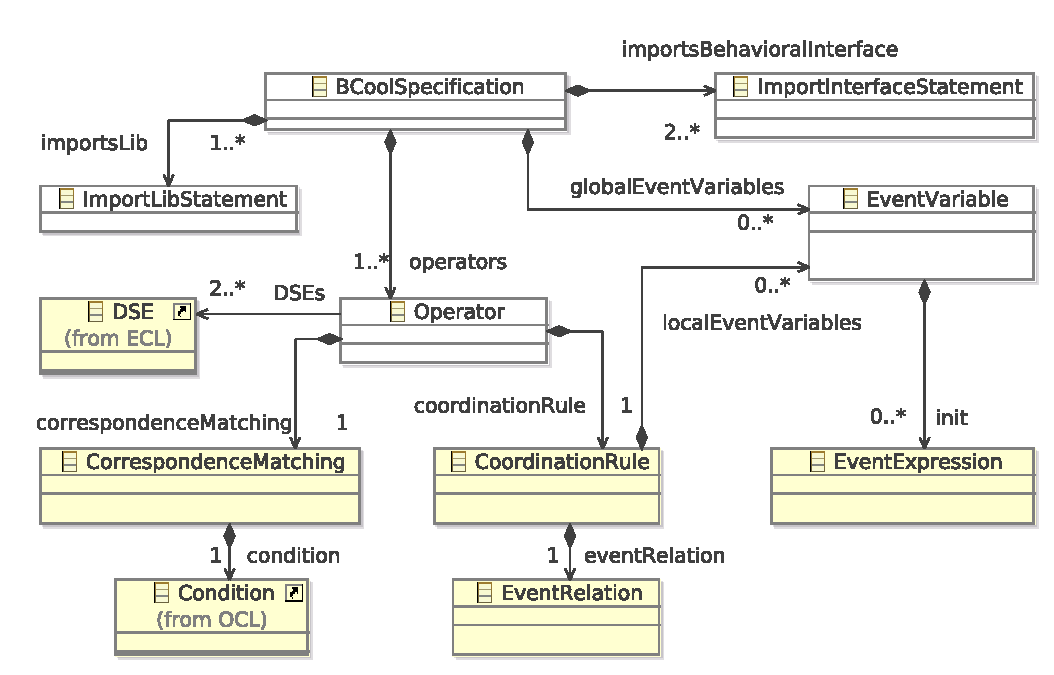
\includegraphics[width=.8\textwidth]{bcool/figs/BcoolMM}
	\caption{Simplified View of \bcool Abstract Syntax}
	\label{fig:bcool}
\end{figure}

The abstract syntax of \bcool is defined by its metamodel (see Figure~\ref{fig:bcool}). The root element is a \emph{BCoolSpecification} that contains \emph{Operators}. Each operator refers to \dse to specify what event types it coordinates. To get the \dse, a \bcool specification imports language behavioral interfaces (\emph{importsInterfaceStatements}). The number of imported interfaces is related with the number of models that the specification accepts as input. Since the \bcool specification is applied at least between two models, it imports at least two interfaces. The same interface can be imported several times to allow the specification of operators between homogeneous languages.   

To build the running example operator, we need to synchronize FSMEvents and Actions. This is done by coordinating instances of \dse \emph{occurs} and instances of \dse \emph{executeIt}. To specify this in \bcool, we first define a specification named \emph{TFSMAndActivity} and we import the language behavioral interface of each language, named \emph{activity} and \emph{tfsm} (Listing~\ref{lst:bcoolrunningexample}: line 3 and 4). Then, the operator \emph{SyncFSMEventsAndActions} is defined, which refers to the \dse \emph{occurs} and \emph{executeIt}, mapped as \emph{FSMEventOccurs} and \emph{ActionExecute} respectively (Listing~\ref{lst:bcoolrunningexample}: line 5). 
	
	 
	\begin{lstlisting}[language=bcool,
	caption={\bcool specification of the running example operator between the TFSM and Activity languages},
	label={lst:bcoolrunningexample}, 
	basicstyle=\scriptsize\ttfamily, backgroundcolor=\color{LGrey}, numbers=left, xleftmargin=2pt]
	BCOoLSpec TFSMAndActivity
	ImportLib "facilities.moccml"
	ImportInterface "activitySemantics.ecl" as activity
	ImportInterface "TFSM.ecl" as tfsm
	Operator SyncFSMEventsAndActions(ActionExecute:activity::executeIt, FSMEventOccurs:tfsm::occurs)
	when (ActionExecute.name = FSMEventOccurs.name);
	do   RendezVous(ActionExecute, FSMEventOccurs)
	end operator
	\end{lstlisting}
	
In \bcool, operators are used to specify when and how instances of the referred \dse must be coordinated. To do so, each operator contains a \emph{correspondence matching} and a \emph{coordination rule}. The former is used to select instance of \dse and the latter to express how the selected instances must be coordinated. 
	
A \emph{correspondence matching} selects instances of \dse by using a \emph{Condition} that contains an OCL Boolean expression. To express the boolean expression, the context of the \dse can be queried to get a specific syntactic element, \eg attribute \emph{name}. The boolean condition is thus used to compare the queried elements. The correspondence matching acts as a precondition for the coordination rule, \ie it is a predicate that defines when the coordination rule must be applied to the given instances of \dse. For instance, for the running example, we query the context of the \dse to get the attribute \emph{name} (Listing~\ref{lst:bcoolrunningexample}: line 6). Then, the attributes are used as operands for the boolean condition. When an instance of \dse \emph{occurs} and an instance of \dse \emph{executeIt} have the same name, the pairs are selected and the coordination rule is applied.
	
The \emph{coordination rule} specifies how the selected instances of \dse must be coordinated. To do so, it contains an \emph{EventRelation} and possibly some \emph{EventVariables} (\emph{localEventVariables}).    	
	
The event relation is used to restrict the relative order of the occurrences of events used as parameters. Its actual parameters can be instances of \dse, some \emph{EventVariables} and/or constants (\eg integer constants). For example, the running example operator must specify a strong synchronization between the events. To express that, we use the event relation \emph{Rendezvous} between the selected instances of \dse \emph{occurs} and \emph{executeIt} (Listing~\ref{lst:bcoolrunningexample}: line 7). This relation accepts two events as arguments and forces the occurrences of these events to happen simultaneously. To illustrate this, Figure~\ref{fig:runningrdv} partially shows the resulting coordination when the running example operator is used to coordinate the models of the coffee machine. In the figure, the occurrences of the \mse \emph{selectCoffee:occurs} and \emph{selectCoffee:executeIt} are forced to happen simultaneously.   
	
	\begin{figure}[h]
		\center
		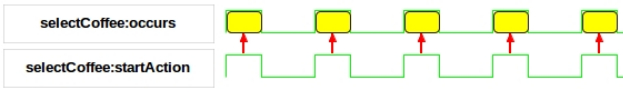
\includegraphics[width=.8\textwidth]{bcool/figs/runningrdv}
		\caption{Resulting coordination of the Coffee Machine by using the event relation Rendezvous}
		\label{fig:runningrdv}
	\end{figure}


Conjointly with an event relation, \bcool enables the definition of \emph{EventVariables} to express more complex coordination rules. An event variable can be either defined locally within the coordination rule (\emph{localEventVariables}) or globally for the whole specification (\emph{globalEventVariables}). These variables either define global events used across different operators, or create a new event from the selected instances of \dse and possibly from attributes of the input models. The definition of these events is made by using an \emph{EventExpression}. An event expression returns a new event from given parameters. For instance, this can be used to select only some occurrences of a \dse instance, thus allowing the implementation of filters. An event expression can also be used to join in a single event the occurrences of different events (union). When used in the coordination rule, the resulting events can be used as parameters of event relations, constraining by transitivity (some of) the occurrences of \dse instances.

To illustrate the use of event variables, we suppose the situation in which the coordination between events relies on a global synchronization clock. This is often the case in synchronous digital systems in which a clock signal is used to coordinate the actions in a circuit. Thus, we slightly modify the running example operator by considering the case in which the coordination between instances of \dse \emph{occurs} and instances of \dse \emph{executeIt} relies on a global clock signal. The selected instances of \dse \emph{occurs} (the \emph{sampledEvent}) are sampled by a global clock (the \emph{trigger}). This results in a new event that ticks always in coincidence with the \emph{trigger}. Each of its occurrences represents the last occurrence of the \emph{sampledEvent} sampled by the \emph{trigger}. 
	
\begin{lstlisting}[language=bcool,
caption={\bcool specification of an operator that illustrates the use of Event Variables},
label={lst:bcoolrunningexampletimed}, 
basicstyle=\scriptsize\ttfamily, backgroundcolor=\color{LGrey}, numbers=left, xleftmargin=2pt]
BCOoLSpec TimedTFSMandActivity
ImportLib "facilities.moccml"
ImportInterface "activitySemantics.ecl" as activity
ImportInterface "TFSM.ecl" as tfsm
Global Event globalClock;
Operator SyncFSMEventsAndActions(ActionExecute:activity::executeIt, FSMEventOccurs:tfsm::occurs)
when (dse1.name = dse2.name);
do
	Local Event sampledOccurs = SampledOn (FSMEventOccurs, globalClock);
	RendezVous(ActionExecute, sampledoccurs)
end operator
\end{lstlisting}
			
To specify this in \bcool, we define a new specification named \emph{TimedTFSMandActivity} (Listing~\ref{lst:bcoolrunningexampletimed}). We first define a global event variable named \emph{globalClock} (Listing~\ref{lst:bcoolrunningexampletimed}: line 5). This global event variable represents the global synchronization clock. Then, in the coordination rule, we use the globalClock together with the \dse \emph{occurs} to create a new local event named \emph{sampledOccurs} (Listing~\ref{lst:bcoolrunningexampletimed}: line 9). To initialize this local variable, we use the event expression \emph{SampleOn}. This expression accepts two events as parameters: the \emph{SampledEvent} and the \emph{Trigger}. The expression creates a new event by sampling the \emph{SampledEvent} by the \emph{Trigger} event. This results in a new event that ticks always after the \emph{SampledEvent} and coincides with the occurrences of the \emph{Trigger} event. In our case, we sample the select instances of the \dse \emph{occurs} (\ie \emph{SampledEvent}) by the event global clock (\ie \emph{Trigger}), which results in the local event variable \emph{sampledOccurs}. Then, in the coordination rule, we coordinate the instances of \dse \emph{executeIt} and the resulting local event \emph{sampledOccurs} by a Rendezvous (Listing~\ref{lst:bcoolrunningexampletimed}: line 10). 

To illustrate the resulting coordination, we use this specification to coordinate the models of the coffee machine. Figure~\ref{fig:runningeventvar} shows the partial resulting coordination between the \mse \emph{selectCoffee:occurs} and \emph{selectCoffee:executeIt} when a global clock is used. The occurrences of the event \emph{selectCoffee:occurs} are sampled by globalClock (in blue in Figure~\ref{fig:runningeventvar}). This results in a new occurrence of the event \emph{sampledOccurs} (in orange in Figure~\ref{fig:runningeventvar}). Then, occurrences of the event \emph{sampledOccurs} are strongly synchronized with the event \emph{selectCoffee:executeIt} (in red in Figure~\ref{fig:runningeventvar}). 

		\begin{figure}[h]
			\center
			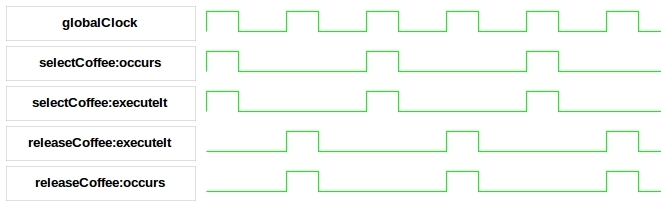
\includegraphics[width=.9\textwidth]{bcool/figs/runningeventvar}
			\caption{Resulting coordination of the Coffee Machine by using the global event variable globalClock}
			\label{fig:runningeventvar}
		\end{figure}



In this subsection, we have presented the abstract syntax of \bcool by relying on the running example operator. To specify this example, we used event expressions and relations that are defined in the library \emph{facilities.moccml} (Listing~\ref{lst:bcoolrunningexampletimed}: line 2). In \bcool, expressions and relations are defined in dedicated libraries that must be imported (\emph{ImportedLibStatement} in Figure~\ref{fig:bcool}). We introduce the notion of library in the following subsection.
	
	
	
%This subsection presents the syntactic elements of \bcool. The abstract syntax of \bcool is defined by its metamodel (see Figure~\ref{fig:bcool}). The metamodel is a particular implementation of the framework for coordination pattern approaches presented in Chapter~\ref{ch:framework}.  
	
%The root element is a \emph{BCoolSpecification} that contains \emph{Operators}. Each operator refers to \dse to specify what event types it coordinates. To get the \dse, a \bcool specification imports language behavioral interfaces (\emph{importsInterfaceStatements}). The number of imported interfaces is related with the number of models that the specification accepts as input. Since the \bcool specification is applied at least between two models, it imports at least two interfaces. The same interface, however, can be imported several times. This allows the specification of the coordination between homogeneous languages.  

%Each operator refers at least two \dse. We decide this implementation from the experimentation. 
%In \bcool, operators are used to specify when and how the referred \dse must be coordinated. To do so, each operator contains a \emph{correspondence matching} and a \emph{coordination rule}. The former is used to select instance of \dse and the latter to express how the selected instances must be coordinated. 

%A correspondence matching relies on a \emph{Condition} that contains an OCL Boolean expression. To express the boolean expression, an integrator can navigate through the context of the \dse to query a specific syntactic element, \eg attribute \emph{name}. The boolean condition is thus used to compare the queried elements. It acts as a precondition for the coordination rule, \ie it is a predicate that defines when the coordination rule must be applied to the given instances of \dse.

%The coordination rule contains the specification of the ``glue'' that coordinates instances of \dse. To express the glue, the coordination rule contains an \emph{EventRelation} and some \emph{EventVariables} (\emph{localEventVariables}). Event relations are used to restrict the relative order of the occurrences of events used as parameters. Its actual parameters can be instances of \dse, some \emph{EventVariables} and/or constants (\eg integer constants). Event relations are defined into a library that the integrator must import (\emph{ImportLibStatement}). The library is defined by using \moccml~\cite{moccmlbib} (Model of Concurrency and Communication Language). The notion of library is discussed in Subsection~\ref{subsec:bcoollib}.



%To illustrate the syntactic elements previously presented, we used \bcool to develop the running example operator, which is defined between the TFSM and Activity languages. We defined a \bcool specification named \emph{TFSMAndActivity} (see Listing~\ref{lst:bcoolrunningexample}) and we imported the language behavioral interface of each language. To do so, we imported the \ecl specification of each language and we named them \emph{activity} and \emph{tfsm}. Also, we imported the \moccml library \emph{facilities.moccml} that provides the event relations that are used latter for the coordination rule. 

%To specify the operator, we have to compare and coordinate FSMEvents and Actions by relying on theirs name. We specify so by defining an operator named \emph{SyncFSMEventsAndActions} that refers to the \dse \emph{FSMEvent::occurs} and \emph{Action::executeIt} and we mapped them as \emph{FSMEvenOccurs} and \emph{ActionExecute} respectively. Then, to select pair of instances of these \dse, we query their context to get the attribute \emph{name}. The attributes are used as operands for a boolean condition. When an instance of \dse \emph{occurs} and an instance of \dse \emph{executeIt} have the same name, the pairs are selected and the coordination rule is applied. To express a strong synchronization between the selected instances, we use the event relation \emph{Rendezvous}. This event relation accepts two events as arguments and forces the occurrences of these events to happen simultaneously. This relation is defined into the library.  



%The specification previously presented can be used to coordinate any pair of TFSM and Activity. In particular, we use it to coordinate the tfsm \emph{CoffeeCoin} and the activity \emph{CoffeeAlgorithm}. Figure~\ref{fig:runningrdv} shows the resulting coordination between the \mse \emph{selectCoffee:occurs} and \emph{selectCoffee:executeIt} in which the occurrences of these events happen simultaneously.  

%To support more complex coordination rules, \bcool enables the definition of new events by using \emph{EventVariables}. Such events can be either defined globally for the whole specification (\emph{globalEventVariables}) or locally within a coordination rule (\emph{localEventVariables}). When globally defined, event variables can be used to define global events used across different operators as synchronization variables. Local event variables, however, can be used in the coordination rule to create a new event from the selected instances of \dse and possibly from attributes of the input models. Then, they can be used as parameters of event relations, constraining by transitivity (some of) the occurrences of \dse instances. 

%Event variables can be initialized by using an \emph{EventExpression}. An event expression returns a new event from given parameters, which can be instances of \dse, some EventVariable and/or constants (\eg integer constants). For instance, an event expression can be used to filter the occurrences of a \dse instance, also, they can also be used to join in a single event the occurrences of different events (union). Event expressions are defined into a \moccml library that must be imported.   

%To illustrate the use of event variables, we modify the running example operator by considering the case in which the coordination between FSMEvents and Actions relies on a global clock signal. This situation is often in synchronous digital systems where a clock signal is used to coordinate the actions in a circuit. In this case, instances of FSMEvents and executeIt are still strongly synchronized, however, such synchronization happens only when a global clock ticks. To specify this in \bcool, we first define a global event variable named \emph{globalClock} (Listing~\ref{lst:bcoolrunningexampletimed}: line 5). Then, in the coordination rule, we use the globalClock together with the \dse \emph{occurs} and \emph{executeIt} to create two local event variables named \emph{sampledExecuteIt} and \emph{sampledOccurs} (Listing~\ref{lst:bcoolrunningexampletimed}: line 9 and 10). To initialize these local variables, we use the event expression \emph{SampleOn}. This expression accepts two events as parameters: the \emph{SampledEvent} and the \emph{Trigger}. \todo{The expression creates a new event by sampling the \emph{SampledEvent} with the \emph{Trigger} event. Then, in the coordination rule, we coordinate the resulting local events by a Rendezvous. However, such a coordination can be gather for future implementation by relying on a library. We the library notion in the following.}


    


	%\item  For example, in some cases only some occurrences of the selected events may be synchronized. Also, it may happen that the coordination relies on a global clock. 
	
	%\item This situation is often in synchronous digital systems where a clock signal is used to coordinate the actions in a circuit. In these cases, it would be necessary to do something on the selected instances of \dse before to apply the event relation. 
	
 

%	\item These variables either define global events used across different operators, or create a new event from the selected instances of \dse and possibly from attributes of the input models. 
	
	
	
	%\item  For instance, an event expression can be used to filter the occurrences of a \dse instance. An event expression can also be used to join in a single event the occurrences of different events (union). 
	
	%\item When used in the coordination rule, the resulting events can be used as parameters of event relations, constraining by transitivity (some of) the occurrences of \dse instances. Event expressions are also defined into \moccml libraries that must be imported. 
	
	
	%\item We illustrate the use of event variables by modifying the previous example. In this case, the synchronization of FSMEvents and Actions is based on a global clock signal. The coordination happens only when the global clock ticks. To do so, we need to define a global event variable that act as global clock, and then, modify the coordination rule. 
	
	%\item First, we define a global event variable named \emph{globalClock}(Listing~\ref{lst:bcoolrunningexampletimed}: line 5). Then, in the coordination rule, we use the globalClock together with the \dse \emph{occurs} and \emph{executeIt} to create two local event variables named \emph{sampledExecuteIt} and \emph{sampledOccurs} (Listing~\ref{lst:bcoolrunningexampletimed}: line 9 and 10). To initialize them, we rely on the event expression \emph{Sample}. 
	
	%\item TODO: What does sample do? 
	
	%\item How local events are syncronized 
	
	%\item However, such a coordination can be gather for future implementation by relying on a library. We the library notion in the following.
	
	%\item The resulting events tick if and only if the global clock and the instance of \dse have also ticked. For instance, the event \emph{sampledOccurs} only ticks if globalClock and the instance of \dse \emph{occurs} ticks. In this case, we use a global event variable together with event expressions to sample the occurrences of selected instances of \dse. Then, we can use the local events as parameters of event relations, constraining by transitivity (some of) the occurrences of \dse instances. In our example, we force a simultaneous occurrence between the local events by using the relation rendezvous (Listing~\ref{lst:bcoolrunningexample2}: line 13). As a result, instances of \dse occurs and startAction happen simultaneously (see Figure~\ref{fig:runningeventvar}). 



%The main element of \bcool (see Figure~\ref{fig:bcool}) is a \emph{BCoolSpecification} that contains language behavioral interfaces (\emph{importsInterfaceStatements}) and \emph{Operators}. The specification must import at least two language behavioral interfaces. Interfaces provide the \emph{DSE} needed for the coordination. The imported \dse serve as parameters for the operators. Then, an operator specifies what instances of these \dse are selected and how they are coordinated (the \emph{DSEs} reference). For instance, to build the running example, we synchronize FSMEvents and the starting of Actions. This is done by coordinating the instances of \dse \emph{occurs} and \emph{startAction} (see Appendix~\ref{ap:languages}). To do so, in a \bcool specification named \emph{SyncFSMEventsAndActions} (Listing~\ref{lst:bcoolrunningexample}: line 1), we import the language behavioral interface of TFSM and Activity (Listing~\ref{lst:bcoolrunningexample}: line 3 and 4). Then, we define the operator named \emph{SyncProduct} with \emph{occurs} and \emph{startAction} as parameters  (Listing~\ref{lst:bcoolrunningexample}: line 6). 

%Each operator contains both a \emph{correspondenceMatching} and a \emph{coordinationRule}. The former relies on a Boolean \emph{Condition} defined as an OCL expression. It acts as a precondition for the coordination rule, \ie it is a predicate that defines when the coordination rule must be applied to the given parameters. To specify the predicate, it is possible to navigate through the context of the \dse and query a specific element used within the Boolean expression. For instance, for the running example, the condition selects pairs of instance of \dse \emph{occurs} and \emph{startAction} by looking at its attribute \emph{name} (Listing~\ref{lst:bcoolrunningexample}: line 7). %This corresponds with a correspondence that relies on a naming convention. We call such a correspondence implicit, however the correspondence may be explicit, we study that case in Section~\ref{subsubsec:explicitcorrespondence}.

%The \emph{coordinationRule} specifies how the selected instances of \dse must be coordinated. To do so, the user must define \emph{EventRelation} and some \emph{EventVariables} (\emph{localEventVariables}).

%Event relations restrict the occurrences of the events on which it is applied. The actual parameters of the event relation can be some instances of \dse and/or some \emph{EventVariables}. For instance, in the running example we want a strong synchronization between FSMEvents and Actions. Thus, the coordination rule uses a ``rendez-vous'' relation between the selected instances of \dse \emph{occurs} and \emph{startAction} (see Appendix~\ref{ap:expressionandrelations}). As a result, all the occurrences of these events are forced to happen simultaneously. Figure~\ref{fig:runningrdv} shows the resulting coordination in the case of the coffee machine. The instance of \dse \emph{occurs} and \emph{startAction} happens simultaneously.

%Lots of other relations, more or less complex can be defined, \eg \emph{Causality}, \emph{FIFO} or ad-hoc relations for specific protocols. For instance, Figure~\ref{fig:runningrunningcausality} illustrates the resulting coordination if we use the event relation \emph{Causality}. The definition of event relations is made in dedicated libraries, which must be imported (see Section~\ref{subsec:bcoollib}).


\subsection{Library}
\label{subsec:bcoollib}

\begin{figure}
	\center
	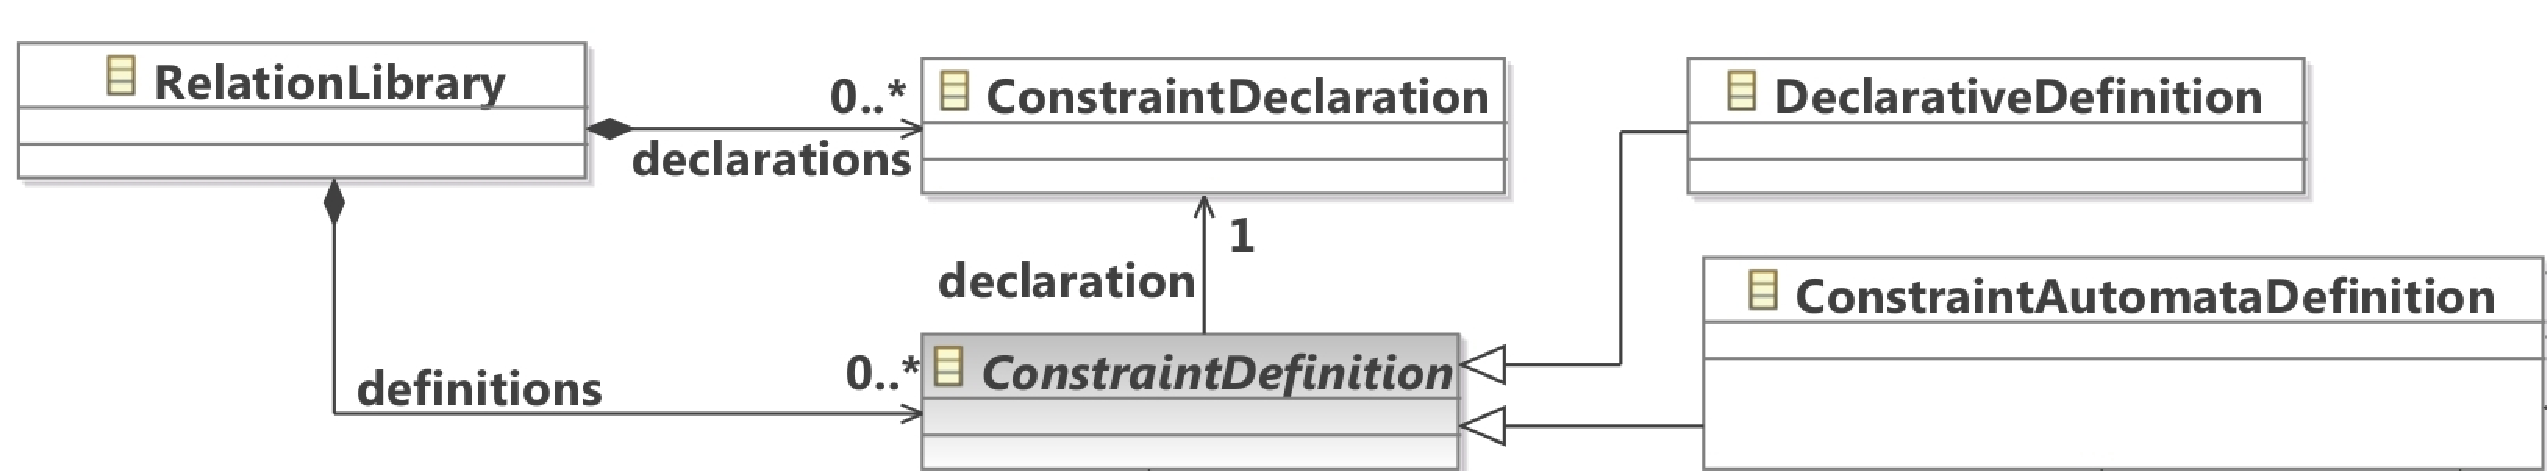
\includegraphics[width=.8\textwidth]{bcool/figs/moccmlmm}
	\caption{Excerpt of MoCCML Metamodel}
	\label{fig:moccml}
\end{figure}

Libraries are used to gather predefined event expressions and relations that can be imported by a \bcool specification (\emph{ImportedLibStatement} in Figure~\ref{fig:bcool}). \bcool relies on \moccml~\cite{moccmlbib} to define libraries of constraints between events. In this subsection, we present an overview of the notion of \moccml library.

A \moccml library (\emph{RelationLibrary} in Figure~\ref{fig:moccml}) is a set of declarations together with their formal parameters. It also contains some definitions, which give the actual behavior of the declarations. There are two categories of constraint definitions: the \emph{Declarative Definitions} and the \emph{Constraint Automata Definitions}. A declarative definition is defined as a set of constraint instances. For more details, we refer the reader to~\cite{moccmloperbib} that described the declarative part inspired from the \ccsl language. A Constraint Automata Definition gives state based support for the definition of relations. This helps a language integrator in the definition of coordination protocols that may be complex like, for instance, the AMBA protocol~\cite{ambabus}. 


To illustrate the use of \moccml for the definition of event relations, we propose to rewrite the coordination rule presented in Listing~\ref{lst:bcoolrunningexampletimed} by defining an automata relation named \emph{RendezvousWithGlobalClock}. The relation accepts three events as parameters: \emph{sampled}, \emph{trigger} and \emph{executeIt}. The \emph{sampled} event identifies the event that will be sampled by the \emph{trigger}. The \emph{executeIt} event identifies the event that is forced to occur simultaneously with the last sample of the \emph{sampled} event. The automata representation is made of two states: \emph{waitSampled} and \emph{waitTrigger} (see Figure~\ref{fig:moccmllib}). In \emph{waitSampled}, the event \emph{trigger} and \emph{sampled} are both allowed to tick but not the \emph{executeIt} event. When the event \emph{sampled} happens, such occurrence will be sampled by the next occurrence of the event \emph{trigger}. This is represented by the transition from \emph{waitSampled} to \emph{waitTrigger}. In this state, the event \emph{trigger} and \emph{executeIt} are forced to happen simultaneously. This represents the sampling of the last occurrence of the \emph{sampled} event. Conversely, in this state, the event \emph{sampled} is forbidden to occur~\footnote{For this example, we chose to forbid the occurrences of the \emph{sampled} event in the WaitTrigger state to prevent missing samples.}. By using this event relation, we rewrite the coordination rule as shown in Listing~\ref{lst:bcoolrunningexamplellib}; the FSMEventOccurs is the \emph{sampled} event, the globalClock is the \emph{trigger} event and the ActionExecute is the \emph{executeIt} event. Figure~\ref{fig:libvcd} shows the resulting coordination of the models of the coffee machine by using the relation RendezvousWithGlobalClock. In blue, we show the occurrences of the \emph{selectCoffee:occurs} (sampled event) that are sampled by global clock (trigger event). When an occurrence is sampled, this makes the event \emph{selectCoffee:executeIt} (executeIt event) to occur simultaneously with the occurrence of the global clock (in red in Figure~\ref{fig:libvcd}). This represents the sampling of the last occurrence of the event \emph{selectCoffee:occurs}.   

\begin{figure}
	\center
	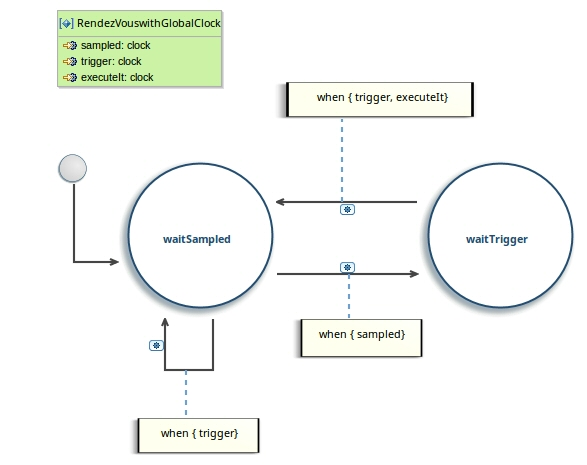
\includegraphics[width=.7\textwidth]{bcool/figs/moccmllib.jpg}
	\caption{State-based representation of the relation \emph{RendezvousWithGlobalClock}}
	\label{fig:moccmllib}
\end{figure}

\begin{lstlisting}[language=bcool,
caption={\bcool specification of the modified running example operator between the TFSM and Activity languages by using the library},
label={lst:bcoolrunningexamplellib}, 
basicstyle=\scriptsize\ttfamily, backgroundcolor=\color{LGrey}, numbers=left, firstnumber=8, xleftmargin=2pt]
do: 
	RendezVouswithGlobalClock(FSMEventOccurs, globalClock, ActionExecute)
end operator
\end{lstlisting}

  
\begin{figure}
	\center
	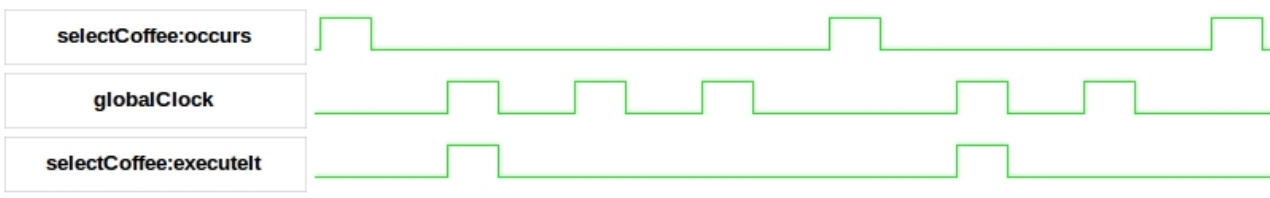
\includegraphics[width=.9\textwidth]{bcool/figs/libvcd}
	\caption{Resulting coordination of the Coffee Machine by using the automata relation \emph{RendezvousWithGlobalClock}}
	\label{fig:libvcd}
\end{figure}


%Listing~\ref{lst:moccmllib} shows a partial representation of the \moccml library \emph{facilities.moccmllib} that provides all the declarations used in the previous examples. Lines 2 and 3 imports \ccsl libraries that contains the declaration of the kernel relations and expression from \ccsl. 

%However, an integrator may need to extend the current library to define new specific constraints depending on its problems and domain. 

%To do so, we use \moccml to define a new event relation named \emph{RendezvousWithGlobalClock} (Listing~\ref{lst:moccmllib}: line 10) that accepts three events as parameter: \emph{ActionExecuting}, \emph{FSMEventTriggering} and \emph{globalClock}. Roughly speaking, the relation synchronizes the events ActionExecuting and FSMEventTriggering by relying on the ticking of globalClock. Then, the coordination rule can be rewritten as shown in Listing~\ref{lst:bcoolrunningexamplellib}. The order of the parameters corresponds with the order of the parameters in the declaration (Listing~\ref{lst:moccmllib}: line 10). 

Libraries enable integrators to organize all relevant event relations and expressions by modeling domains. This improves the readability of a \bcool specification by gathering domain specific relations, which can be reused in other specification. By relying on a \moccml library, the application of \bcool operators results in a \ccsl specification. We can use \ccsl tool (\eg TimeSquare\cite{timesquarebib}) to analyze and execute the generated coordination model. In the next subsection, we further explain how the coordination model is generated by presenting the semantics of \bcool.   



%We could also use another language to build the semantics of coordination rules and then take benefit from other analysis tools. In the following section, we present the semantics of \bcool by showing how the generation of a model of coordination is done from a \bcool specification. 

%Libraries enable integrators to organize all relevant event relations and expressions by modeling domains. This improves the readability of a \bcool specification by gathering domain specific relations, which can be reused in other specification.
	
%Event expressions create a new event from their parameters (\eg building the \textit{Union}, or the \textit{Intersection} of its parameters).%Relations, however, constrain the evolution of events given as actual parameters. 
%By relying on \moccml, the application of \bcool operators generate a coordination specification in \ccsl. We can then use \ccsl tool (TimeSquare~\cite{timesquarebib}) to perform analyze and execute the generated coordination specification. This is further discussed in Section~\ref{sec:validation}.

%\begin{lstlisting}[language=moccml,
%		caption={Facilities Library in \moccml},
%		label={lst:moccmllib}, 
%		basicstyle=\scriptsize\ttfamily, backgroundcolor=\color{LGrey}, numbers=left, xleftmargin=2pt]
%		AutomataConstraintLibrary Facilities{ 
%		import "platform:/plugin/fr.inria.aoste.timesquare.ccslkernel.model/ccsllibrary/kernel.ccslLib" as kernel;
%		import "platform:/plugin/fr.inria.aoste.timesquare.ccslkernel.model/ccsllibrary/CCSL.ccslLib" as CCSLLib;
%		RelationLibrary CCSLBasedBCOoLRelations {
%		RelationDefinition RendezVouswithGlobalClockDef[RendezVouswithGlobalClock]{ 
%			Expression sampledActionExecuting = SampledOn (Sampled -> globalClock, Trigger-> ActionExecuting)
%			Expression sampledOccurs = SampledOn (Sampled -> globalClock, Trigger-> FSMEventTriggering)
%			Relation RendezVousSamples[Coincides](Clock2-> sampledActionExecuting , Clock1->FSMEventTriggering)
%		}
%		RelationDeclaration RendezVouswithGlobalClock (ActionExecuting: clock , FSMEventTriggering: clock, globalClock: clock)
%		}
%		}
%\end{lstlisting}

\subsection{Execution Semantics}
In this subsection, we describe the execution semantics of \bcool, \ie how a \bcool specification is used to generate a coordination model. To illustrate the different steps in the generation, we rely on the application of the running example operator (see Listing~\ref{lst:bcoolrunningexample}) between the models of the coffee machine.

\begin{figure}
	\center
	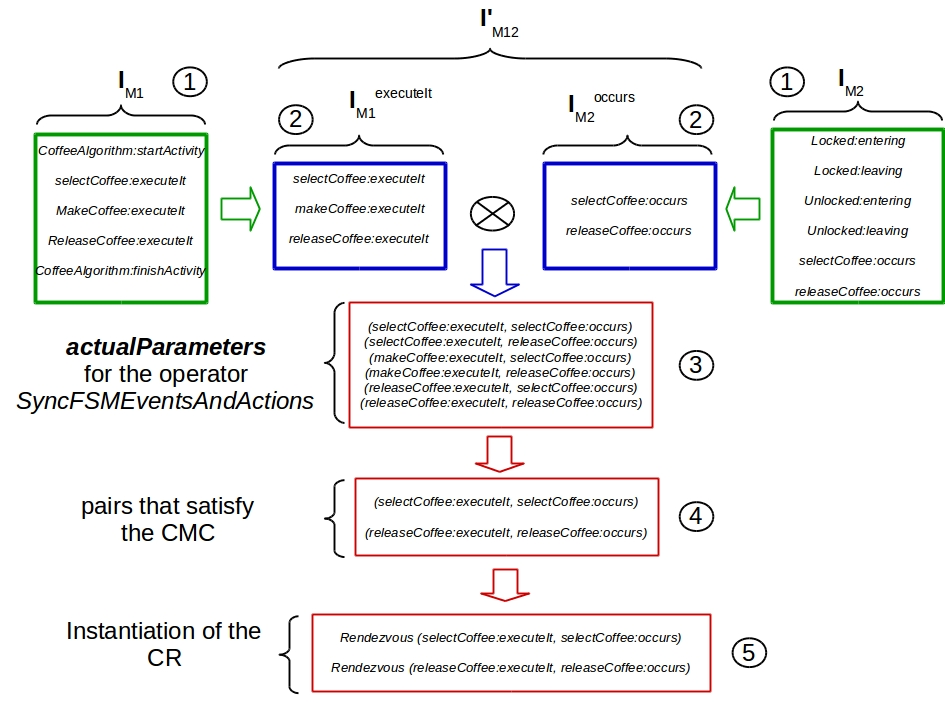
\includegraphics[width=1\textwidth]{bcool/figs/semantics}
	\caption{Steps in the application of the \bcool specification between the models of the coffee machine}
	\label{fig:semantics}
\end{figure}

Let $Ev$ be the (finite) set of event type names (representing the \dse). Considering a language $L$, A behavioral interface $i_L$ is a subset of event type names, $i_L \subset Ev$. A \bcool specification imports $N$ disjoint language interfaces, with $N\geq 2$. Also, a \bcool specification contains a set of operators $\mathcal{O}p$. Each operator from $\mathcal{O}p$ has a set of formal parameters $\mathcal{P}$, where each parameter is defined by a name and its type (\ie an event type). Each operator also has a correspondence matching condition (denoted $CMC$) and a correspondence rule (denoted $CR$). A \bcool specification is applied to a set of input models denoted $\mathcal{M_I}$, with $|\mathcal{M_I}| = N$.

From an operational point of view, the first step consists in producing the model behavioral interface of each input model. It results in a set of model interfaces denoted $\mathcal{I_{M_I}}$, of size $N$. An interface is a set of events, each of which is typed by an event type. For instance, when the running example operator is applied between the models of the coffee machine, the first step consists in extracted the \mse of the Activity \emph{CoffeeAlgorithm} and the TFSM \emph{CoffeeCoin} that results in two sets of \mse named respectively $\mathcal{I_M}{1}$ and $\mathcal{I_M}{2}$ (step 1 in Figure~\ref{fig:semantics}).

Each operator $op$ in $\mathcal{O}p$ is processed individually and several times with different actual parameters, which depend on the model interfaces in $\mathcal{I_{M_I}}$. The set of actual parameters to be used is obtained by a \emph{restricted} Cartesian product of all the model interfaces in $\mathcal{I_{M_I}}$. The restriction consists in two steps: First, a new set of model interface (denoted $\mathcal{I^{'}_{M_I}}$) is created. For each parameter $p$ in $\mathcal{P}$, a new model interface $\mathcal{I^{\textit{\text{p}}}_{M_I}}$ is created and all the events in $\mathcal{I_{M_I}}$ that have the same type than $p$ are collected in $\mathcal{I^{\textit{\text{p}}}_{M_I}}$. Then, $\mathcal{I^{\textit{\text{p}}}_{M_I}}$ is added to $\mathcal{I^{'}_{M_I}}$ (step 2 in Figure~\ref{fig:semantics}). For instance, the running example operator has as parameters the event types \emph{Action::executeIt} and \emph{FSMEvent::occurs}. Thus, the set $\mathcal{I^{'}_{M_I}}$ is composed of two set named $\mathcal{I_M}{1}{executeIt}$ and $\mathcal{I_M}{1}{occurs}$ that corresponds respectively with events of type \emph{Action::executeIt} and \emph{FSMEvent::occurs} (step 2 in Figure~\ref{fig:semantics}).
%

Second, a classical Cartesian product is applied on $\mathcal{I^{'}_{M_I}}$. It results in a set containing the list of actual parameters to be used with the operator, \ie each set in the result of the Cartesian product represents the actual parameters of the operator (step 3 in Figure~\ref{fig:semantics}). For each set $actualParams$ in the result of the Cartesian product, if $actualParams$ satisfies the correspondence matching condition ($CMC$), then the coordination rule ($CR$) is instantiated with the values in $actualParams$. Returning to the running example operator, the correspondence matching condition is used to select \mse by comparing the instances names. This results in two selected sets: \emph{selectCoffee:occurs} and \emph{selectCoffee:executeIt}, and  \emph{releaseCoffee:occurs} and \emph{releaseCoffee:executeIt} (step 4 in Figure~\ref{fig:semantics}). The coordination rule is instantiated two times. The instantiation is made in two steps. First, the local events, if any, are created in the targeted coordination language according to the expression used to initialize it. The expression can use any event in $actualParams$ and possibly some constants (\eg some Integer constants). The local events are added to $actualParams$ so that they can be used in the next. The second step is the application of the relation. It results in the creation of the corresponding relation in the targeted coordination language. The actual parameters of the coordination rule are then the ones from $actualParams$ or some constants, like for the expressions. For the coffee machine, the event relation rendezvous is instantiated twice; one time for each set in $actualParams$ that satisfies the $CMC$ (step 5 in Figure~\ref{fig:semantics}).

Currently, the application of a \bcool operator generates a \ccsl specification that represents the coordination. Listing~\ref{lst:runningexampleccsl} shows the partial \ccsl specification for the coffee machine. The specification begins by importing the \ccsl specification of each model (Listing~\ref{lst:runningexampleccsl}: line 3 and 4). Then, the main block contains the coordination specification that is made of two instances of the event relation rendezvous (Listing~\ref{lst:runningexampleccsl}: line 9 and 11). Notice that individual specification of each model are not modified. So that, the behavior of individual models is not altered. Instead, the coordination adds some constrains thus restricting the behavior of models, but it does not add new behaviors. This results in a generated coordination that is not intrusive (\ie exogenous).

In this section, we have presented the abstract syntax and the semantics of \bcool. Also, we have presented \moccml for the definition of libraries. In the next section, we present the current implementation of \bcool as a set of Eclipse plugins into the GEMOC studio. 
%In the next section, we present the \bcool framework which is an Eclipse environment that enables the developing of \bcool operator between languages and automate the coordination between language. 




\begin{lstlisting}[language=moccml,
caption={Resulting \ccsl specification for the coffee machine system},
label={lst:runningexampleccsl}, 
basicstyle=\scriptsize\ttfamily, backgroundcolor=\color{LGrey}, numbers=left, xleftmargin=2pt]
ClockConstraintSystem TFSMandActivity {
imports {
import "facilities.moccml" as lib;
import "coffeeCoin.extendedCCSL" as coffeeCoin;
import "coffeeAlgorithm.extendedCCSL" as coffeeAlgorithm;
}
entryBlock mainBlock
	Block mainBlock {
		Block coffeeCoincoffeeAlgorithmsublock {
			Relation  SyncFSMEventsAndActionselectCoffee_executeItselectCoffee_occurs [ RendezVous ]
			( ClockA -> "coffeeAlgorithm::selectCoffee_executeIt", ClockB -> "coffeeCoin::selectCoffee_occurs")
			Relation  SyncFSMEventsAndActionsreleaseCoffee_executeItreleaseCoffee_occurs [ RendezVous ]
			( ClockA -> "coffeeAlgorithm::releaseCoffee_executeIt", ClockB -> "coffeeCoin::releaseCoffee_occurs")}}
}
\end{lstlisting}    

\section{Validation}
\label{sec:validation}

In this section, we use the \bcool specification presented in Listing~\ref{lst:bcoolrunningexample} to coordinate the running example. The application of \bcool operators generates a coordination specification in \ccsl. Listing~\ref{lst:runningexampleccsl} partially shows the generated \ccsl specification. Note that the individual specification are imported (Listing~\ref{lst:runningexampleccsl}: line 3 and 4) whereas the coordination only adds some constraints (Listing~\ref{lst:runningexampleccsl}: line 9). The behavioral model of each model remains untouched. 
	
\begin{lstlisting}[language=moccml,
	caption={Resulting \ccsl specification for the running example},
	label={lst:runningexampleccsl}, 
	basicstyle=\scriptsize\ttfamily, backgroundcolor=\color{LGrey}, numbers=left, xleftmargin=2pt]
ClockConstraintSystem SyncProductTFSM-fUMLOperatorsCoordination {
imports {
	import "coffeeCoin.extendedCCSL" as coffeeCoin;
	import "coffeeAlgorithm.extendedCCSL" as coffeeAlgorithm;
}
	entryBlock mainBlock
	Block mainBlock {
	 Block coffeeCoincoffeeAlgorithmsublock {
		Relation SyncProductselectCoffee_startselectCoffee_occurs [ RendezVous ]
				( ClockA -> "coffeeAlgorithm::selectCoffee_startAction",
				  ClockB -> "coffeeCoin::selectCoffee_occurs")
		Relation SyncProductreleaseCoffee_startActionreleaseCoffee_occurs [ RendezVous ]
				( ClockA -> "coffeeAlgorithm::releaseCoffee_startAction",
				  ClockB -> "coffeeCoin::releaseCoffee_occurs")
					}
				}
			}
\end{lstlisting}    
		
The \ccsl specification can be executed by using TimeSquare~\cite{timesquarebib}. Figure~\ref{fig:coffemachinevcd} illustrates the partial timing output of the execution of the running example. TimeSquare also offers the possibility to obtain by exploration quantitative results on the scheduling state-space (see Figure~\ref{?}). The state space is always computable if models are finite. 
	 
\begin{figure}[h]
	 	\center
	  	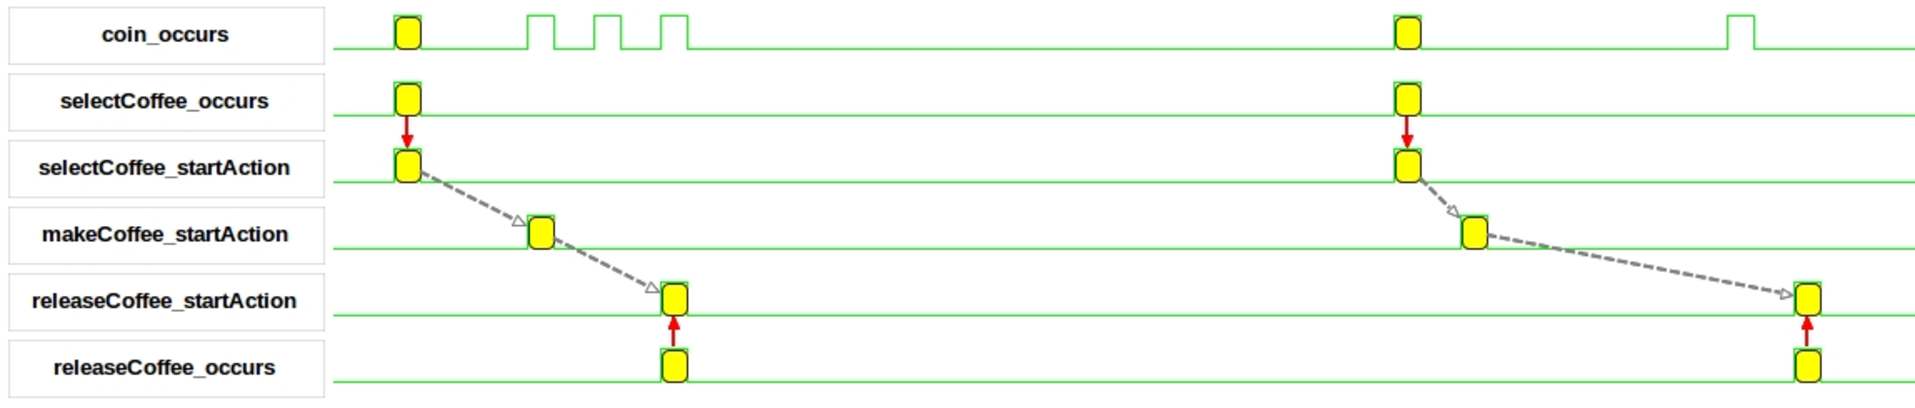
\includegraphics[width=.9\textwidth]{bcool/figs/coffeemachinevcd}
	  	\caption{Resulting timing execution of the coordinated system}
	  	\label{fig:coffemachinevcd}
\end{figure}
	
When a coin is inserted (\emph{coin:occurs} happens), the \emph{selectCoffee:occurs} event is triggered. Then, the coordination forces a simultaneous occurrence between \emph{selectCoffee:occurs} and \emph{selectCoffee:startAction} thus making the activity starts to execute. Then, when the coffee is released, the coordination forces a simultaneous occurrence between the events \emph{releaseCoffee:startAction} and \emph{releaseCoffee:occurs}. The coordination constrains some events by making them to happen simultaneously. This reduces what can be done by individual models, \ie some FSMEvents and Action can only occurs simultaneously. Other events are only constrained by the individual semantics. The coordination constraints the behavior of models without adding new ones. In this sense, the coordination is non intrusive thus not altering the behavior of individual models. 

\todo{To show the space state. To illustrate the last paragraph by showing the state space}

\todo{Recheck state space!}


\section{Implementation}
\label{section:bcoollengbench}
This section presents the implementation of \bcool into the GEMOC studio\footnote{http://www.gemoc.org}; which integrates technologies based on Eclipse Modeling Framework (EMF)~\footnote{http://eclipse.org/modeling/emf/} adequate for the specification of executable domain specific modeling languages. The studio includes a \emph{language workbench} to design and implement tool-supported xDSMLs and a \emph{modeling workbench} where the xDSMLs are automatically deployed to allow designers to edit, execute, simulate, and animate their models~\cite{ttc15bib}. \bcool takes advantages of this collaborative environment by adding coordination facilities. The resulting integrated environment enables the implementation of the workflow presented in Figure~\ref{fig:proposedworkflow} in which a language integrator uses the language workbench to develop \bcool operators to specify coordination patterns between languages, and then a system designer can use these operators in the modeling workbench to  coordinate models. In this section, we illustrate the use the of language workbench by developing the running example operator (see Listing~\ref{lst:bcoolrunningexample}). Then, in the modeling workbench, we use this operator to execute and verify the models of the coffee machine. 

\begin{figure}[h]
	\begin{center}
		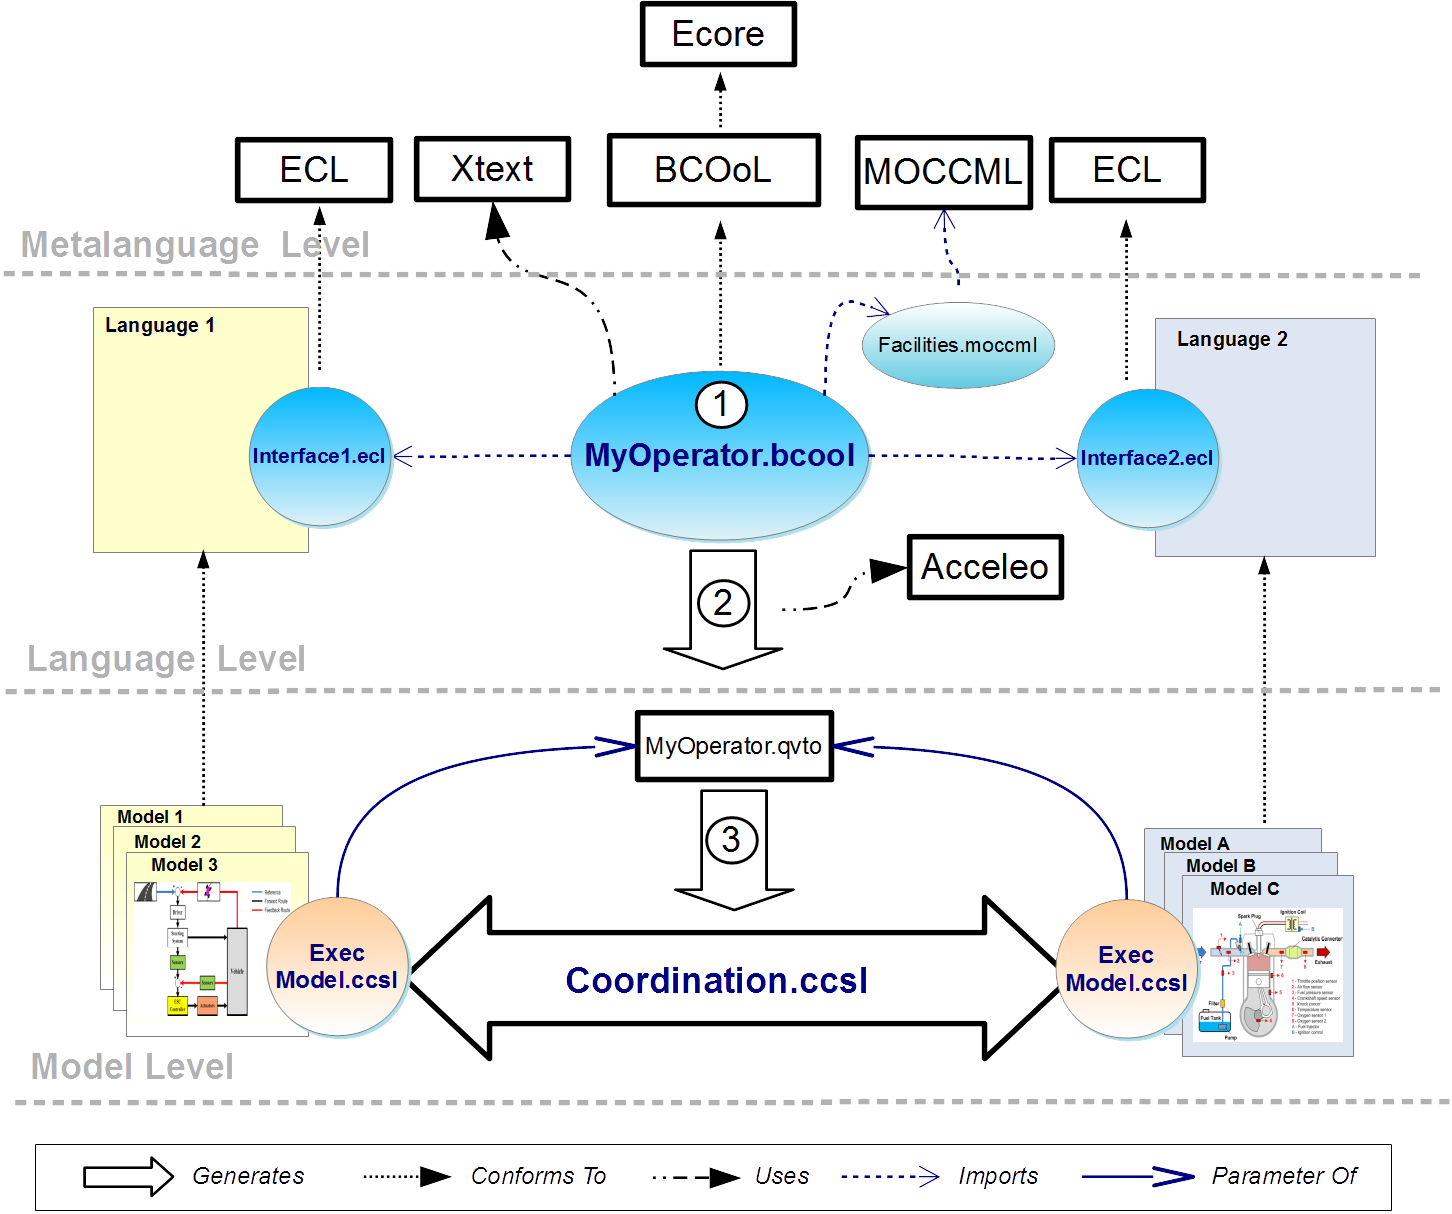
\includegraphics[width=1\textwidth]{bcool/figs/bcooltechnos}
		\caption{Overview of the \bcool Framework}
		\label{fig:bcooltechnos}
	\end{center}
\end{figure}

\bcool is developed as a set of plugins based on the EMF (at top of Figure~\ref{fig:bcooltechnos}). The \bcool abstract syntax has been developed using Ecore (\ie the metalanguage associated with EMF) and the textual concrete syntax has been developed in Xtext~\footnote{http://eclipse.org/Xtext/}, thus providing advanced editing facilities. For the running example operator, we use the TFSM and Activity languages that are integrated into the studio. Then, we use \bcool to specify the Listing~\ref{lst:bcoolrunningexample}. In the \bcool specification, we can import the language behavioral interfaces of each language that are automatically deployed (Figure~\ref{fig:bcooltechnos}: step 1). In addition, the language workbench provides \moccml thus helping the integrator to specify relations and expression.      

%When languages are deployed into the language workbench, an integrator can define a new \bcool specification and then import the language behavioral interfaces that are automatically deployed (Figure~\ref{fig:bcooltechnos}: step 1). Also, the language workbench provides \moccml thus helping the integrator to specify relations and expression. For the running example, we use the TFSM and Activity languages that are integrated into the studio. 
	\begin{lstlisting}[language=bflow,
	caption={\bflow specification for the models of the coffee machine},
	label={lst:bflowcoffeemachine}, 
	basicstyle=\scriptsize\ttfamily, backgroundcolor=\color{LGrey}, numbers=left, xleftmargin=2pt]
	BCOoLFlow CoffeeMachine
	ImportBCOoL  "TFSMAndActivity.bcool" ;
	Model CoffeCoin "coffeecoin.tfsm"
	Model CoffeeAlgorithm "coffeeAlgorithm.ad"
	Flow 
	applies SyncFSMEventsAndActions between (CoffeeAlgorithm, CoffeCoin);
	end Flow;
	\end{lstlisting}


In the modeling workbench, a system designer can use \bcool operators to automate the coordination of models. To ease this task, we provide a simple language named \bflow that enables a system designer to specify how operators of a \bcool specification are applied on a set of models (Figure~\ref{fig:bcooltechnos}: step 2). Listing~\ref{lst:bflowcoffeemachine} shows the \bflow specification for the models of the coffee machine. The \bflow specification begins by importing the \bcool specification that contains the operators (Listing~\ref{lst:bflowcoffeemachine}: line 2). Then, it specifies the models that will be coordinated. For the running example, this corresponds with the TFSM named \emph{CoffeeCoin.tfsm} and the Activity named \emph{CoffeAlgorithm.ad} (Listing~\ref{lst:bflowcoffeemachine}: line 3 and 4). Then, the specification contains \emph{Flows} that defines which operators are used and on which models are applied. Flows define a sequential order of application of operators. In other words, the first defined flow is the first operator that will be applied and soon on. For instance, in Listing~\ref{lst:bflowcoffeemachine}, line 6 specifies that the operator named \emph{SyncFMEventsAndActions} must be applied between the models CoffeeCoin and CoffeeAlgorithm. This corresponds with the first and the only operator to be applied to coordinate the models of the coffee machine. However, a \bflow specification can contain several flows, this is further discussed in the validation chapter.  


In the modeling workbench, the \bflow specification is used by the \emph{Gemoc Coordinated Execution Engine} to execute the coordinated system (Figure~\ref{fig:bcooltechnos}: step 3). We automate the generation of the coordination by relying on Acceleo\footnote{http://www.eclipse.org/acceleo/} and QVTo\footnote{https://projects.eclipse.org/projects/modeling.mmt.qvt-oml}. First, an acceleo transformation is used to translate the \bcool specification into a QVTo transformation. Then, the QVTo transformation can be applied between models to generate the coordination specification in \ccsl. These steps have been automated by relying on a set of plugins that are integrated into the modeling workbench. To illustrate the use of the Coordinated Execution Engine, we coordinate and execute the models of the coffee machine. First, we configure the launcher that contains information about the \bcool specification, the \bflow specification and the configuration launcher for each model. In Figure~\ref{fig:execenginemenu}, by clicking on \emph{Debug}, the simulation is launched. Then, the engine provides several options to drive the execution of the models. For instance, it provides to the system designer a list of the next valid execution steps (Figure~\ref{fig:runningworkbench}: point 3). Also, the workbench provides the animation of models (Figure~\ref{fig:runningworkbench}: point 4). 

\todo{The modeling workbench also provides tools to analize the resulting \ccsl specification (Figure~\ref{fig:runningworkbench}: point 1). For example, the modeling workbench offers the possibility to obtain by exploration quantitative results on the scheduling state-space of the coordinated system. The exploration of all schedules can be captured explicitly in a state space graph as presented~\ref{fig:statespace}. Any cyclic path in this graph (starting from the initial configuration) represents a valid schedule of the model. The state space is always computable if the behavior of models are finite.}

\begin{figure}[h]
	\centering
	\subfigure[Gemoc Coordinated Execution Engine launcher]{
		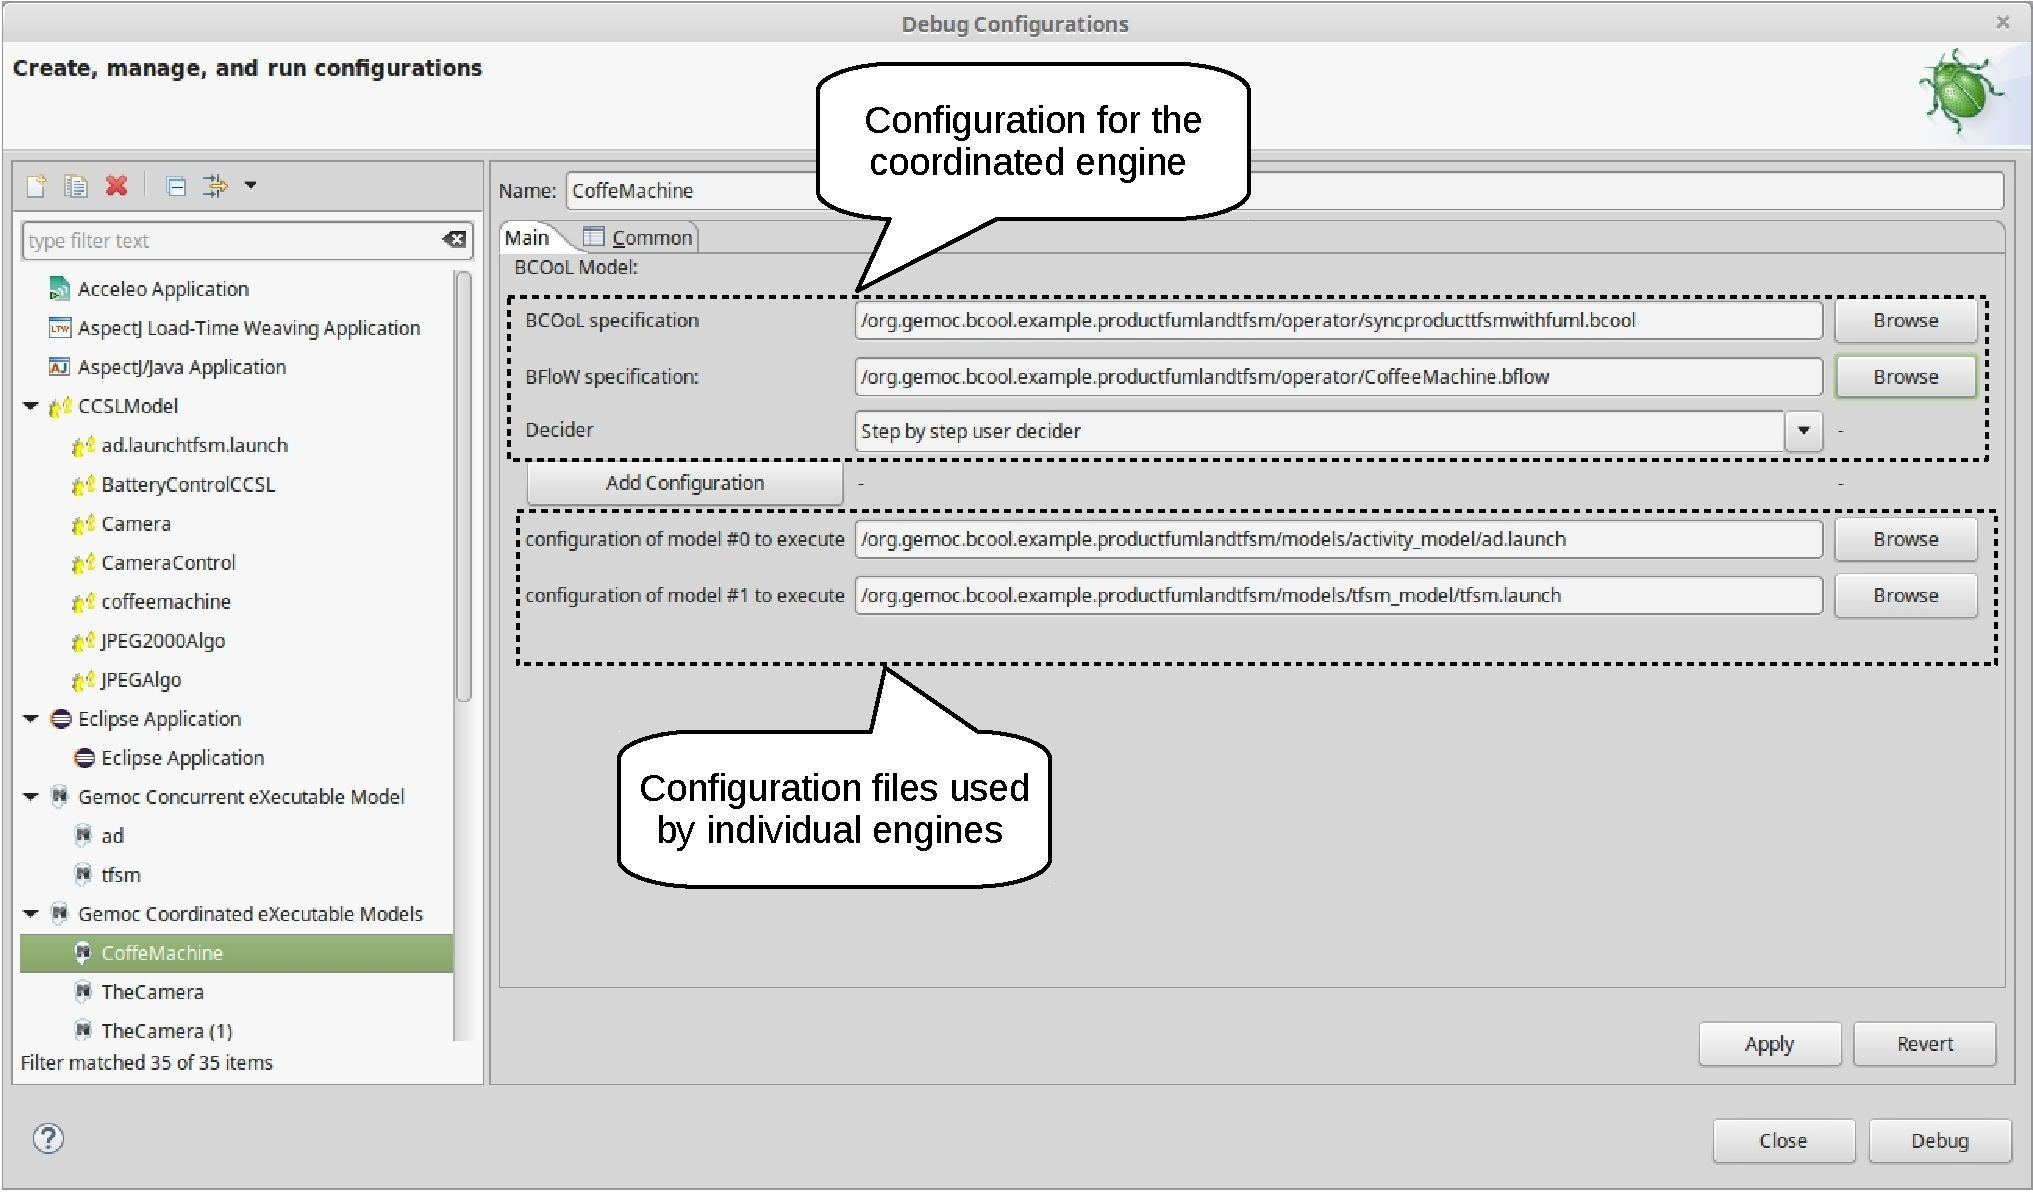
\includegraphics[width=.7\textwidth]{bcool/figs/execenginemenu}
		\label{fig:execenginemenu}
	}
	\subfigure[Coordinated Execution of the models of the Coffee Machine]{
		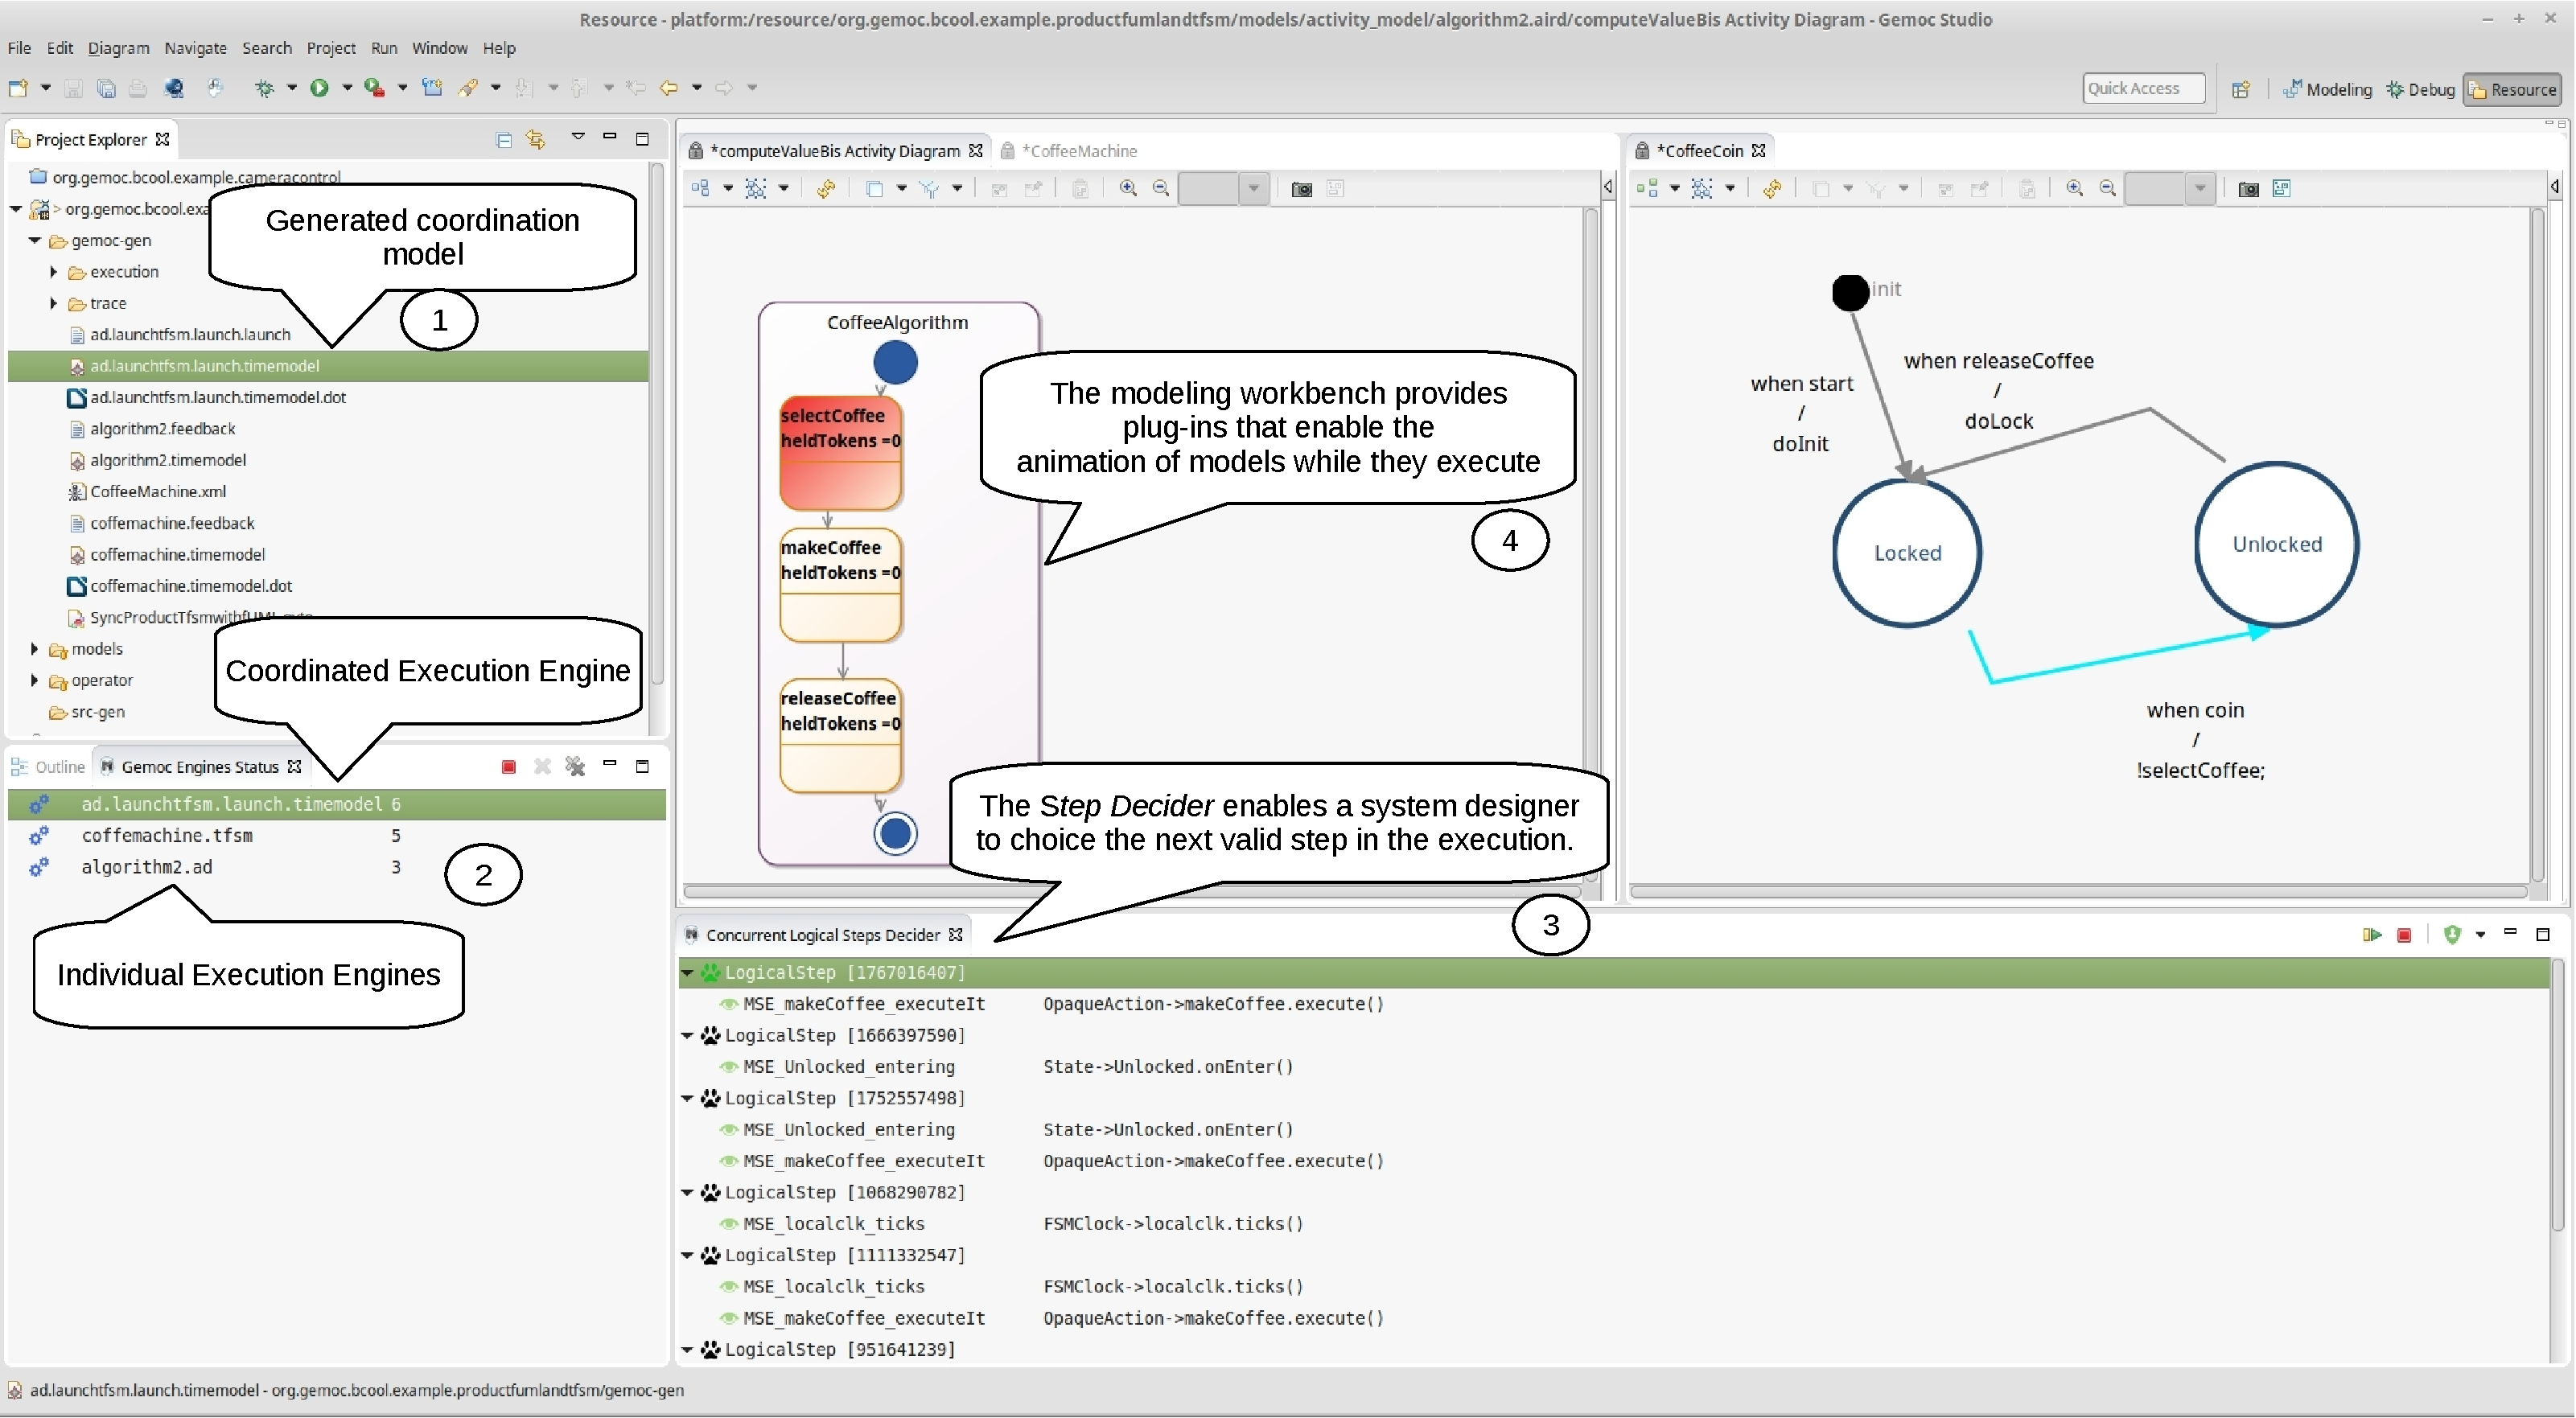
\includegraphics[width=.7\textwidth]{bcool/figs/runningworkbench}
		\label{fig:runningworkbench}
	}
	\caption{Coordinated Execution of models in the Modeling Workbench}
	\label{fig:subfigureExample1}
\end{figure}

\bcool is currently integrated into the GEMOC studio\footnote{The reader can download studio the from http://gemoc.org/studio-download/} that includes the coffee machine as a deployable example. To try it, we need only to download the studio and then to follow the wizard to create a new example project. The project \bcool is hosted on Github\footnote{http://github.com} as part of the GEMOC project\footnote{http://github.com/gemoc/coordination} thus making the source code public and available. In addition, we built a website that contains more examples with full descriptions\footnote{http://timesquare.inria.fr/BCOoL}. For example, it contains a video that presents the whole flow of the coffee machine example. 

In this section, we have presented the current integration of \bcool into the GEMOC studio. The framework eases the task of integrators and system designer to coordination models and languages. Integrators can develop operators between languages that a system designer can use to coordinate and execute their models. In the next section, we compare our approach with coordination languages and coordination frameworks.  

\begin{figure}[h]
	\begin{center}
		\includegraphics[width=.8\textwidth]{bcool/figs/statespace}
		\caption{State space representation of the coordinated model of the coffee machine, encoding the set of valid schedules}
		\label{fig:statespace}
	\end{center}
\end{figure}

%\bcool is developed as set of plugins for Eclipse Modeling Framework (EMF)\footnote{http://www.eclipse.org}. Its abstract syntax has been developed using Ecore (\ie the meta-language associated with EMF) and the textual concrete  syntax has been developed in Xtext, thus providing advanced editing facilities (see Figure~\ref{fig:bcooltechnos}). A \bcool specification is defined between languages by relying on its language behavioral interface made of \dse. To get the \dse, the \ecl specification of each language must be imported (Figure~\ref{fig:bcooltechnos}: point 1). From a \bcool specification, the generation of the coordination between models has been automated by relying on two technologies: Acceleo\footnote{http://www.eclipse.org/acceleo/} and QVTo\footnote{https://projects.eclipse.org/projects/modeling.mmt.qvt-oml}. The acceleo transformation translates the \bcool specification into a QVTo transformation (Figure~\ref{fig:bcooltechnos}: point 2). The transformation can be applied between models to generate the coordination specification in \ccsl (Figure~\ref{fig:bcooltechnos}: point 3).    
	

	
%These technologies has been integrated into the GEMOC Studio, an Eclipse package atop EMF, which includes both a \emph{language workbench} to design and implement tool-supported xDSMLs, and a \emph{modeling workbench} where the xDSMLs are automatically deployed to allow system designers to edit, execute, simulate, and animate their models. In this context, \bcool takes advantages of this collaborative environment by adding coordination facilities. 

%\begin{figure}[h]
%	\begin{center}
%		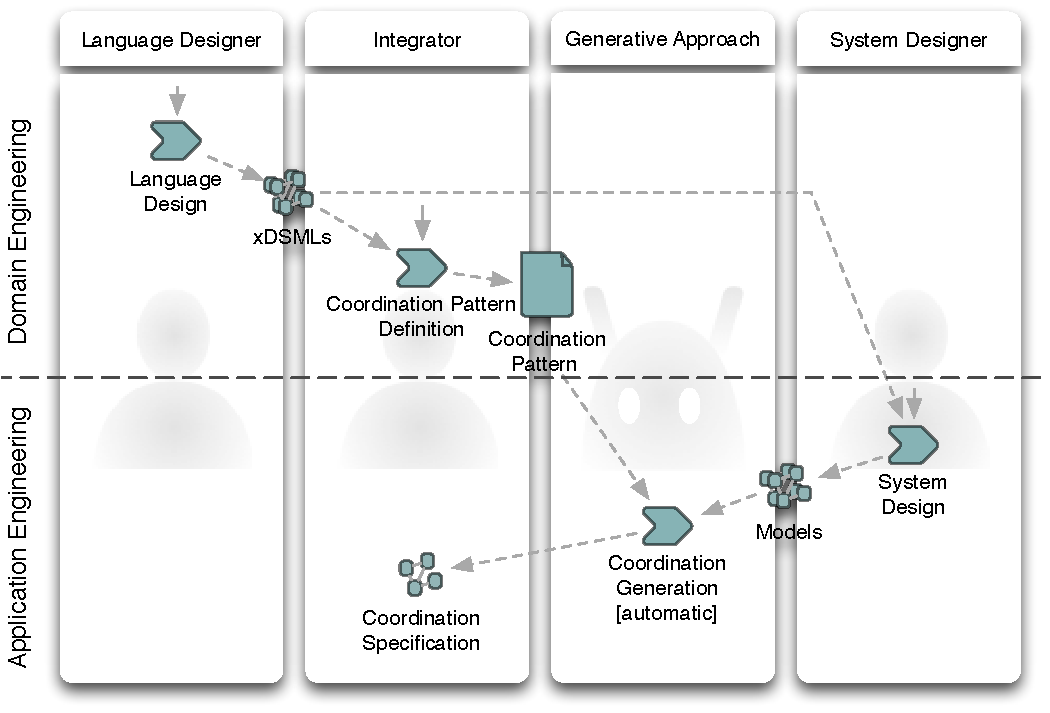
\includegraphics[width=.6\textwidth]{bcool/figs/process}
%		\caption{The Proposed Workflow}
%		\label{fig:proposedworkflow}
%	\end{center}
%\end{figure}

%Based on the GEMOC studio, Figure~\ref{fig:proposedworkflow} illustrates the proposed workflow. Such a workflow relies mainly in two stakeholders: an integrator that uses the language workbench and an system designer that uses the model workbench. 

%In the language workbench, an integrator develop operators by relying on the deployed languages. The \bcool specification can import the language behavioral interface that are automatically deployed into the workbench. To build its own libraries, the workbench provides \moccml thus helping the integrator to specify EventRelations and EventExpression. 

%Operators are automatically deployed into the modeling workbench and can be used by a system designer to generate the coordination. This task is automated by relying on a set of plugins\footnote{\todo{I have to talk about how the operators are applied by the plugin, this is not evident!}}. The workbench provides several tools to perform verification activities \eg execution and animation, space-state exploration, etc.  

%To summarize, a \bcool developer (\ie integrator) develops a set of operators by relying on the language behavioral interface (\ecl) and libraries (\moccml). Then, a \bcool user (\ie system designer) applies these operator on his models to: 
%		\begin{itemize}
%			\item Generate a coordination specification.
%			\item Perform execution and verification activities.
%		\end{itemize}

%We implement the running example in the GEMOC studio. We rely on the languages TFSM and Activity that are integrated into the study. Then, we use \bcool to specify the operator in Listing~\ref{lst:bcoolrunningexample} (Figure~\ref{fig:screenbcool}: point 1). In the model workbench, we build the models of the coffee machine: a TFSM named \emph{CoffeeCoin} and an Activity named \emph{CoffeeAlgorithm} (Figure~\ref{fig:screenbcool}: point 2). Then, we use the workbench to execute, verify and animate the coordinated models. In particular, Figure shows the animation proposed by Sirius.   

%\begin{figure}[h]
%	\begin{center}
%		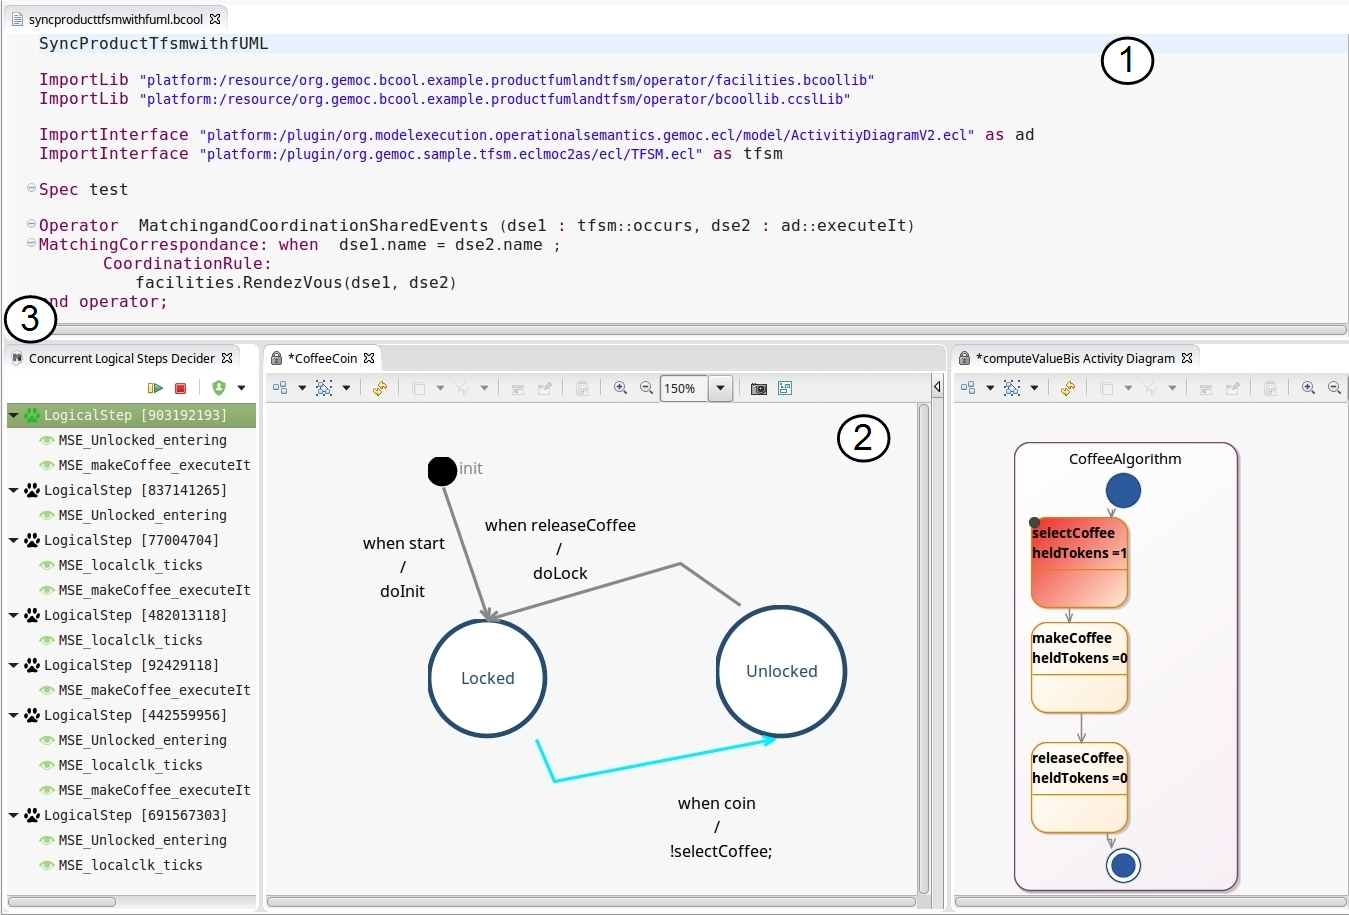
\includegraphics[width=.6\textwidth]{bcool/figs/bcoolscreen.png}
%		\caption{Screenshot}
%		\label{fig:screenbcool}
%	\end{center}
%\end{figure}

%A video presenting the whole flow can be found on the companion website~\footnote{http://timesquare.inria.fr/BCOoL}, which also contains more examples with full descriptions. These examples are hosted in Github~\footnote{http://github.com} at BCOoLExamples~\footnote{http://matiasvara.github.io/BCOoLExamples/}. The \bcool code is hosted in the open source project Gemoc~\footnote{http://github.com/gemoc/} thus making the project fully available.

%\subsection{Flow by using the plugins}
%\subsection{Flow by using ANT}
%	\begin{itemize}
%		\item Ant\footnote{http://www.eclipse.org/eclipse/ant/}
%		\item Operational QVT Ant tasks let you launch QVTO transformations from the Ant script.
%		\item The flow can be implemented by using Ant.
%		\item This enables to define explicitly how a \bcool specification is invoked. 
%		\item However, the specification of a ANT script must be partially defined by the user. For instances, several parameters must be defined by the user, \eg model paths, generated timemodel. 
		  
%	\end{itemize}


 % \begin{figure}[h]
  %	\begin{center}
  %		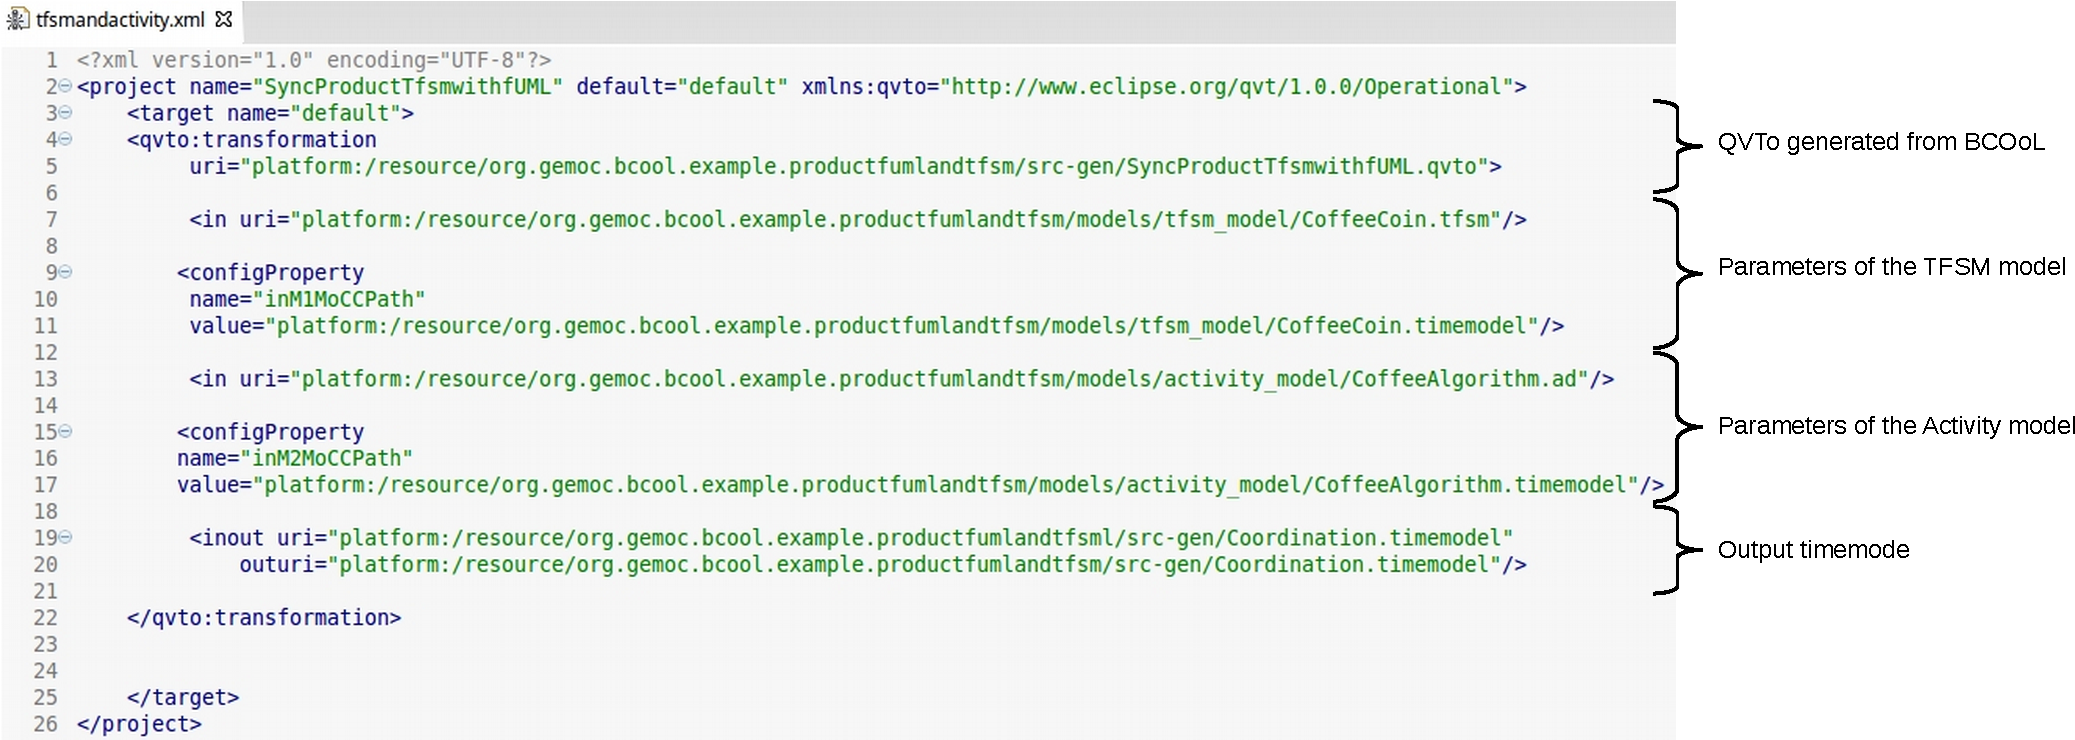
\includegraphics[width=1\textwidth]{bcool/figs/antbcool.pdf}
  %		\caption{ANT script to build the coordination specification for the coffee machine}
  %		\label{fig:screenantbcool}
 % 	\end{center}
 % \end{figure}

\section{Evaluation}
\label{sec:evaluation}
In this section, we evaluate \bcool in term of four criteria:
	\begin{enumerate}
		\item Definition of the coordination between languages, \ie understandability and adaptability of coordination operators. 
		\item Automation of the coordination between models. 
		\item Studies of the coordinated system, \ie analysis capabilities.
		\item Tooling support.
	\end{enumerate}  
We use these criteria to compare our approach with coordination languages and coordination frameworks.

In \bcool, the definition of the coordination between languages is based on operators. In particular, coordination rules explicitly define the semantics of the resulting coordination. Notice that an integrator can vary the semantics of the resulting coordination by only modifying the coordination rules of the operators. In frameworks like Ptolemy, an integrator is unable to change the proposed coordination without modifying the framework itself. For instance, in Ptolemy, this means changing the current implementation of a \emph{director} written in Java. The same problem appears in ad-hoc translational approaches~\cite{dinatale}, where the transformation needs to be changed. Since this state-of-the-art approaches is using general-purpose transformation frameworks, this work needs a good knowledge of coordinated languages as well as a good knowledge of the transformation language itself. This is beyond the expected skills of an integrator. In our approach, we are using a language dedicated to integrator experts thus easing the understanding and adaptation of the \bcool specification. 

The definition of domain specific coordination operators enables the automation of the coordination between models. The manual coordination of models (as proposed by coordination languages) requires an system designer that specifies each relation. The reader can notice that the number of relations increases with the number of model elements involved in the coordination. Our proposition is to leverage this task for the system designer at the language level and then to generate all the required relations accordingly.

%\subsection{Analysis Capabilities}
Regarding system execution and verification, both coordination languages and coordination frameworks allow to execute the coordinated system, however, the verification varies from one approach to another. Some coordination languages rely on a formal language thus providing verification. Differently, in Ptolemy, the main validation method is based on the execution of the coordinated system~\cite{ptoleframebib}. In our approach, by relying on \ccsl, a system designer is able to provide execution and verification of the coordinated system.

%\subsection{Tooling Support}
Current Coordination Frameworks like Ptolemy~\cite{ptoleframebib} and ModHel'X~\cite{modhelxbib} provide a dedicated environment to develop and coordinate heterogeneous models. They rely on a common syntax based on actors and a semantics given by Models of Computation. In addition, they enable the system designer to hierarchical coordinate models. The environments include a graphical editor, an execution engine, plotters and so on. These environments, however, are ad-hoc solutions to manage both the development and the coordination of heterogeneous models. Differently, in our approach, the studio is the integration of several plug-ins that deal with different aspects of the heterogeneous development of models, \eg the GEMOC studio for the design and implementation of DSMLs, the Sirius animator for graphical representation, TimeSquare for the analysis of model execution. Our approach takes advantages of this collaborative environment, and it provides the means for model coordination.


\section{Conclusion}



\chapter{Validation}
\label{ch:examples}
\section{Introduction}
In this chapter, we validate the use of \bcool through the developing of two coordination operators between the TFSM and Activity language. These operators specify a hierarchical coordination pattern between in which states from TFSM are coordinated with Activities. Such patterns are common in coordination frameworks~\cite{giraultbib}, however, their specification is hidden inside a tool. We propose to use \bcool in order to make their specification explicit. We illustrate the use of these operators by coordinating the heterogeneous model of surveillance camera system. This chapter is organized as follows. We begin by presenting the operators together with its \bcool definition. We continue by using these operators to coordinate the model of a surveillance video system. We use the \bcool framework to validate the coordinated model. Then, in the discussion, we compare our approach with current coordination approaches, and finally, we conclude.  
\section{Definition of Coordination Operators between the TFSM and Activity Languages}




\begin{itemize}
	\item This section presents the \bcool specification of three operators between the TFSM and Activity languages. In the following, we describe each operator and we discuss their semantics. We then present the \bcool specification according with the chosen semantics.  
	
	\item The \emph{SyncFSMEventsAndSignals} operator differs from the running example operator because it synchronizes FSMEvents and Signals. Whereas in the running example the occurrences of FSMEvents were synchronized with the starting of Actions, here they are synchronized with the occurrences of Signals, \ie by coordinating instances of \dse \emph{occurs} and \emph{doSignal}. This operator only requires a slight modification of the specification presented in the running example (see Listing~\ref{lst:bcoolrunningexample}). The only modification is the type of the \dse used in the operator (see Listing~\ref{lst:bcoolsigandfsmevents}: line 1). The rest of the definition (\ie the correspondence matching and coordination rule) is unchanged (see Listing~\ref{lst:bcoolsigandfsmevents}: line 2 and 3). We want to highlight that the adaptation has been done only by identifying the new \dse to be constrained. This should also be the case for other coordination pattern.
	

	 
\begin{lstlisting}[language=bcool,
caption={\bcool specification of the \emph{SyncFSMEventsAndSignals} operator},
label={lst:bcoolsigandfsmevents}, 
basicstyle=\scriptsize\ttfamily, backgroundcolor=\color{LGrey}, numbers=left, xleftmargin=2pt]
Operator SyncFSMEventsAndSignals(SignalOccurs:activity::doSignal, FSMEventOccurs:tfsm::occurs)
when (SignalOccurs.name = FSMEventOccurs.name);
do   RendezVous(SignalOccurs, FSMEventOccurs)
end operator
\end{lstlisting}
	 
	 
	 
	 \item The \emph{startActivityWhenEnter} operator specifies a hierarchical coordination pattern between the TFSM and Activity languages, unlike hierarchical coordination frameworks where the semantics is hidden, this operator explicitly specifies how the hierarchical coordination is implemented. In our case, we chose the semantics in which entering a specific state of a TFSM model triggers the execution of a given Activity. When leaving a state, several semantic variation points may be chosen. The outgoing transitions from a state can be considered, for instance, as preemptive for the activity model (\ie firing a transition from a state to another preempts the internal activity). Alternatively, the transition can be considered as non-preemptive (\ie the states cannot be left before the associated activity finishes). In our case, we chose non-preemptive transitions because the activity should not be interrupted until the information has been sent. 
	
	
	 \item We define the \emph{startActivityWhenEnter} (Listing~\ref{lst:bcoolStartActivityWhenEnter}: line 1) operator that coordinates the entering and leaving of a state with the execution of an activity. The entering into a state is identified by the \dse \textit{entering} defined in the context of State. Instances of such \dse have to be coordinated with instances of the \dse \textit{startActivity}. Similarly, leaving a state is identified by \dse \textit{leaving} and finishing an activity is identified by \dse \textit{finishActivity}. To identify pairs of such events, the correspondence matching selects instances of \dse \emph{startActivity} and \emph{finishActivity} by using their context (Listing~\ref{lst:bcoolStartActivityWhenEnter}: line 2). The pairs selected identify the starting and finishing of the same activity. Besides, we select the activities that represent a state by comparing the \emph{onEnterAction} defined in the states and the name of the activities. OnEnterAction is a string defined in the context of State (see Figure~\ref{fig:tfsmmm}) that specifies the method invoked when a state is entered. In our case, we use this attribute to specify the name of the activity that the state represents (Listing~\ref{lst:bcoolStartActivityWhenEnter}: line 2).
	
	 
	 \begin{lstlisting}[language=bcool,
	 caption={Hierarchical operator between TFSM and Activity languages},
	 label={lst:bcoolStartActivityWhenEnter}, 
	 basicstyle=\scriptsize\ttfamily, backgroundcolor=\color{LGrey}, numbers=left, xleftmargin=2pt]
	 Operator  startActivityWhenEnter (activityStart : ad::startActivity , activityStop : ad::finishActivity, enterState : tfsm::entering, leaveState : tfsm::leaving)
	 when ((activityStart = activityStop) and (enterState = leaveState) and (activityStart.name = enterState.onEnterAction));
	 do 
		 ExecuteActivityNonPeemptive (enterState, leaveState, activityStart, activityStop)
	 end operator;
	 \end{lstlisting}
	 
	 \item To coordinate the selected instances of \dse, the coordination rule uses the event relation \emph{ExecuteActivityNonPeemptive}, which is defined in \moccml (see Figure~\ref{fig:looprelation}). The relation takes four events as parameters: the events \emph{modeEnter} and \emph{modeLeave} that represents respectively the entering and leaving of a state; and the events \emph{startActivity} and \emph{finishActivity} that represents respectively the starting and finishing of an activity. The state-based representation is made of two states named \emph{waitEnterState} and \emph{WaitFinishActivity}. In waitEnterState state, the events modeEnter, modeLeave and startActivity are allowed to tick. Only when modeEnter and startActivity happen simultaneously, the state \emph{waitFinishActivity} is reached. In this state, only the finishActivity is allowed to happen. When this event occurs, \ie the activity has finished, the state \emph{waitEnterState} is reached and the modeLeave is allowed to occur. The use of this relation in the coordination rule results in transitions cannot preempt the execution of the internal activities. The entering a state makes the activity to start to execute synchronously. Then, only after the activity has finished, the state can be left.
	 
	 \item We want to highlight that an integrator can vary the semantics of the coordination by only modifying the event relation in the coordination rule. For instance, by slightly modifying the event relation, the transition may become preemptive.
	 
	 \begin{figure}[h]
	 	\center
	 	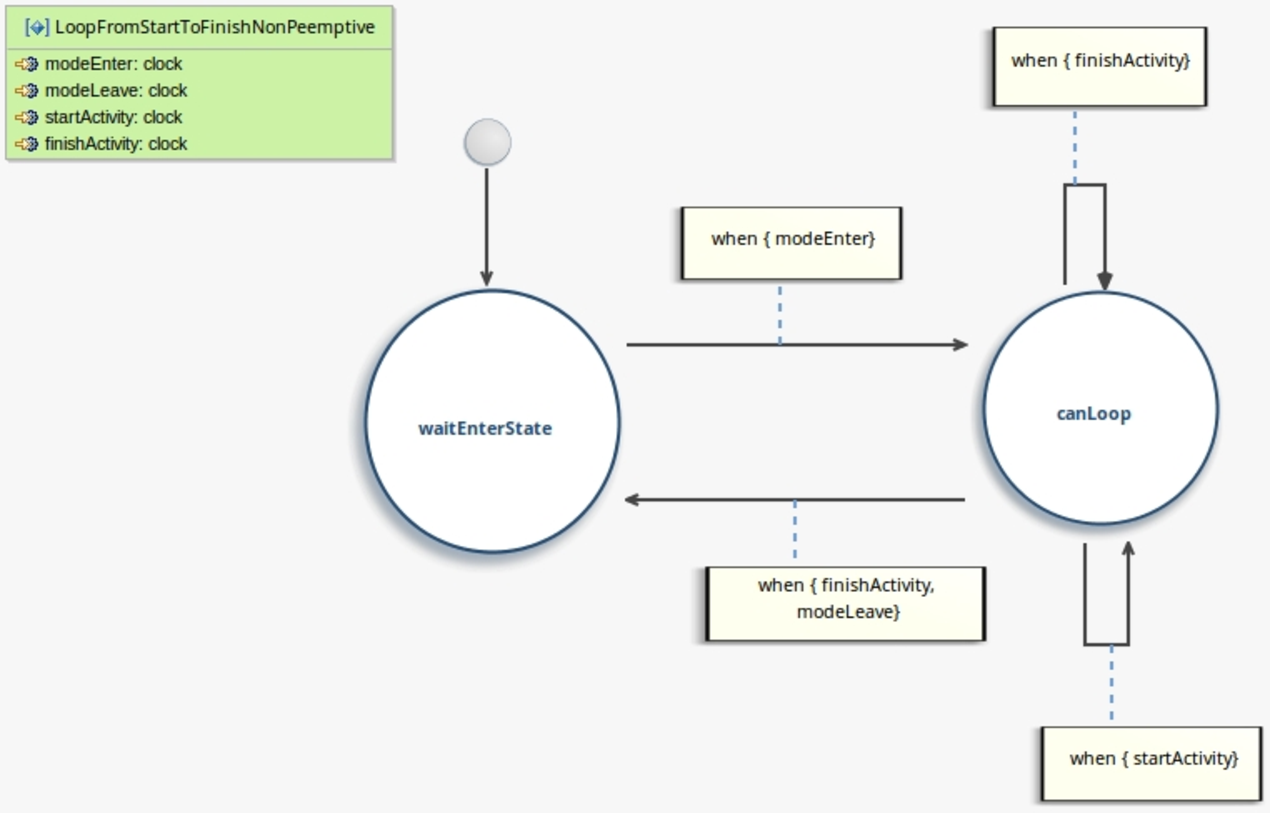
\includegraphics[width=.7\columnwidth]{examples/figs/LoopFromStartToFinishNonPreemptive}
	 	\caption{\emph{ExecuteActivityNonPeemptive} event relation}
	 	\label{fig:looprelation}
	 \end{figure}
	 
	
	 \item In the \emph{AtomicActivity} operator, we deal with the temporal aspects the model coordination. The operator specifies how the time in the TFSM elapses during the execution of an activity. In these languages, the time is represented differently. In the TFSM language, each state machine has a \emph{localClock} used to measure the time while the Activity language is untimed. The local clock is a \emph{FSMClock}, which defines a \dse named \emph{ticks} whose occurrences represent a physical time increment. In the Activity language, the duration of activities can be represented as the time between the \dse \emph{startActivity} and \dse \emph{finishActivity}. To coordinate the time, it is necessary to specify the number of \emph{ticks} of the local clock between the occurrence of the \dse \emph{startActivity} and \emph{finishActivity}. Again, several semantic variation points may be chose. For instance, the coordination rule could express that the execution of the activities takes a fixed amount of time. In our example, we propose to enforce the execution of the activity to be atomic with respect to the time in the TFSM model. As a result, there are no occurrences of the \dse ticks of the corresponding local clock during the execution of the activity.
	 
	 
	 \item In \bcool, we define the operator \emph{AtomicActivity} (Listing~\ref{lst:bcoolAtomicExec}: line 6) that specifies how time is consumed during the execution of the activities. The correspondence matching selects instances of \dse \emph{startActivity} and \emph{finishActivity} by using their context. In this case, the correspondence matching does not filter instances of \dse \emph{ticks}, as a result, the selected activities will be atomic respect to all the instances of \dse \emph{ticks}, \ie to all the clocks in the TFSM. Note that th TFSM language forces to one the number of localClocks in a TFSM. Thus, there is only one instance of \dse \emph{ticks} in each TFSM. 
	 
	 
	 \begin{lstlisting}[language=bcool,
	 caption={Timing operator between TFSM and Activity languages},
	 label={lst:bcoolAtomicExec}, 
	 basicstyle=\scriptsize\ttfamily, backgroundcolor=\color{LGrey}, numbers=left, xleftmargin=2pt, firstnumber=6]
	 Operator AtomicActivity (activityStart : ad::startActivity , activityStop : ad::finishActivity, timeTicks : tfsm::ticks)
	 when (activityStart = activityStop );
	 do 
		 AtomicExec (activityStart, activityStop, timeTicks)
	 end operator;
	 \end{lstlisting}
	 
	 
	 \item To express the coordination rule, we use the event relation \emph{AtomicExec} which makes the execution of the activities atomic with respect to the local clock of the TFSM. We specify this relation in \moccml (see Figure~\ref{fig:atomicexec}). The event relation accepts three events as parameters: \emph{ticks}, \emph{startAct} and \emph{finishAct}. While the event ticks represents the ticking of the local clock, the startAct and finishAct events represent respectively the starting and finishing of an activity. In \emph{waitstartActivity} state, the event ticks is allowed to occur, thus making the time elapse. When the startAct event happens, \ie the activity starts to execute, the \emph{waitfinishActivity} state is reached and the event ticks is forbidden to occur, \ie the time in the TFSM does not elapse while the activity executes. Only when the event finishAct happens, the \emph{waitstartActivity} state is reached, and \emph{ticks} is allowed to occur again. In the operator, we use this relation to make the execution of the activities atomic, \ie there is no occurrence of the \dse ticks of the corresponding local clock during the execution of the activity.
	 
	 
	 
	 \begin{figure}
	 	\center
	 	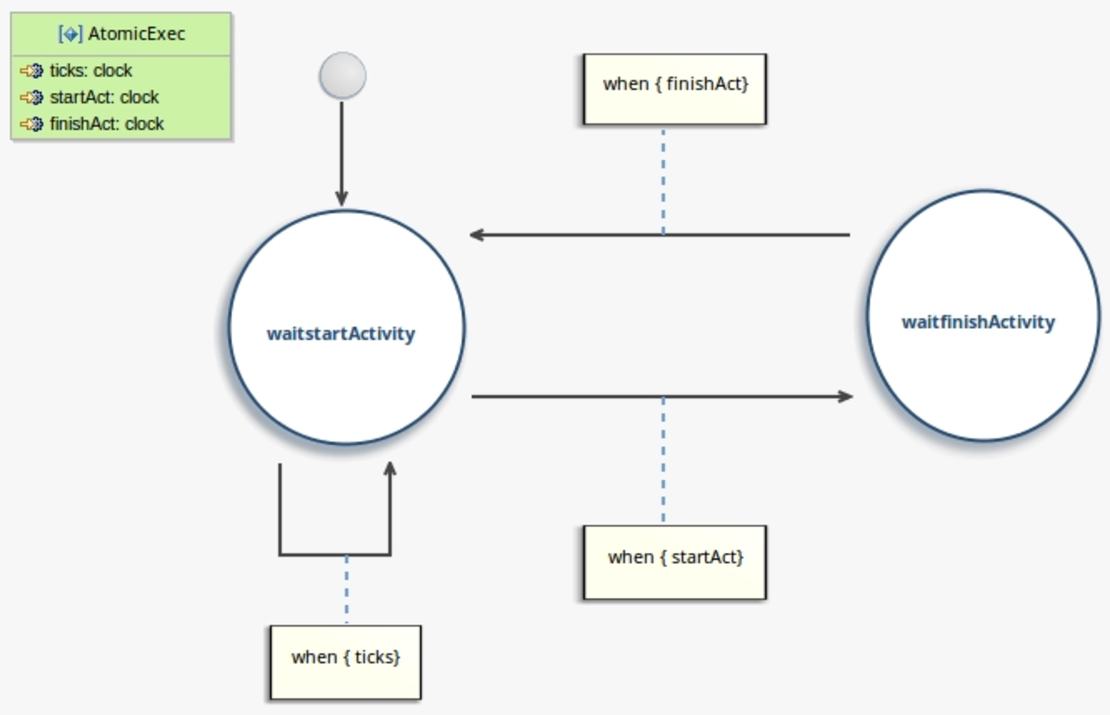
\includegraphics[width=.7\columnwidth]{examples/figs/AtomicExec}
	 	\caption{\emph{AtomicActivity} event relation}
	 	\label{fig:atomicexec}
	 \end{figure}
	 
	 
	 
	 \item In this section, we have used \bcool to define a set of coordination operators that deal with both control and timing aspects of the coordination between TFSM and Activity languages. Unlike hierarchical coordination frameworks where the semantics is hidden, these operators explicitly specified how the coordination is implemented. More precisely, coordination rules explicitly define the semantics of the resulting hierarchical coordination. Furthermore, we ease the definition of relations by using \moccml, a dedicated language to express constraints between events. Thus, an integrator can vary the semantics of the coordination by only modifying the event relation in the coordination rule. Frameworks like Ptolemy do not support such a variation without changing the current implementation of the framework. This means modifying the implementation of a \emph{director} written in Java, which needs a good knowledge of the framework. In our approach, we are using a language dedicated to language integrator experts thus easing the understanding and adaptation of the \bcool specification. In the next section, we use these operators to coordinate and execute the models of the surveillance camera system.
	 
\end{itemize}


  










%Similar than the \emph{startActivityWhenEnter} operator, the \emph{AtomicActivity} operator also defines a coordination between states and activities, but in this case, it deals with the temporal aspects of the coordination. The operator specifies how the time in the TFSM elapses during the execution of the activities that specify the on-entry action of a state. Thus, this coordination is also hierarchical, but in this case, only considers the timing aspects. %In these languages, the time is represented differently. In the TFSM language, each state machine has a \emph{localClock} used to measure the time while the Activity language is untimed. The local clock is a \emph{FSMClock}, which defines a \dse named \emph{ticks} whose occurrences represent a physical time increment. In the Activity language, the duration of activities can be represented as the time between the \dse \emph{startActivity} and \dse \emph{finishActivity}. Thus, to coordinate the time, it is necessary to specify the number of \emph{ticks} of the local clock between the occurrence of the \dse \emph{startActivity} and \emph{finishActivity}. In this operator, we propose to enforce the execution of the ``internal'' activity to be atomic with respect to the time in the TFSM model. As a result, there is no occurrence of the \dse ticks of the corresponding local clock during the execution of the activity. 











%\section{Operators between TFSM and Activity}
	\begin{itemize}
		\item \todo{To show only the hierarchical coordination!}
		\item \todo{This example has to show the benefice of our approach in term of automatic coordination and variations of the semantics of the coordination}
		\item \todo{The no timing hierarchical coordination must be specify in one operator by relying on a library}
			
		\item Operator captures a given coordination pattern between TFSM and the fUML language
		\item We capture a timing and hierarchical coordination pattern.
		\item We use these operators to coordinate a surveillance camera system (Moto)
		\item We verify and verify the coordinated system.

	\end{itemize}
	
	
	\subsection{Definition}
	
	In a \bcool specification (see Listing~\ref{fig:bcoolsyncrohetero}: line 1), we define four coordination operators between the TFSM and fUML languages. The specification begins by importing (see Listing~\ref{fig:bcoolsyncrohetero}: line 3 and 4) the behavioral interfaces of each language, defined as an \ecl specification.
	
	
	\todo{The first operator, named \emph{SyncProduct} (see Listing~\ref{fig:bcoolsyncrohetero}: line 6), differs from the running example because it applies to heterogeneous languages (namely fUML and TFSM). 
	Whereas in the running example the occurrences of FSMEvents were synchronized with the occurrences of other FSMEvents, here they are synchronized with the start of fUML \emph{Actions}, \ie by coordinating instances of \dse \emph{occurs} and \emph{startAction}.} 

	For the second and third operators, we specify a hierarchical coordination pattern between the TFSM and fUML languages, unlike hierarchical coordination frameworks where the semantics is hidden, these operators explicitly specify how the hierarchical coordination is implemented. In our case, we chose the semantics in which entering a specific state of a TFSM model triggers the execution of a given fUML activity. When leaving a state, several semantic variation points may be chosen. The outgoing transitions from a state can be considered, for instance, as preemptive for the activity model (\ie firing a transition from a state to another preempts the internal activity). Alternatively, the transition can be considered as non-preemptive (\ie the states cannot be left before the associated activity finishes). In this paper, we chose non-preemptive transitions, preemptive ones are detailed on the companion webpage. Listing~\ref{fig:bcoolnopremtive} presents the \bcool specification that is organized around two operators: \textit{StateEntering} and \textit{StateLeaving}. 
	
	\begin{lstlisting}[language=bcool,
	caption={Heterogeneous synchronized product operator between the TFSM and fUML languages},
	label={fig:bcoolsyncrohetero}, 
	basicstyle=\scriptsize\ttfamily, backgroundcolor=\color{LGrey}, numbers=left, xleftmargin=2pt]
	BCOoLSpec TFSM-fUMLOperators
	ImportLib "facilities.bcoollib"
	ImportInterface "activitySemantics.ecl" as activity
	ImportInterface "TFSM.ecl" as tfsm
	
	Operator SyncProduct(dse1 : activity::startAction, dse2 : tfsm::occurs)
	CorrespondenceMatching: when(dse1.name = dse2.name)
	CoordinationRule: RendezVous(dse1, dse2)
	end operator
	\end{lstlisting}
	
	
	
	\begin{lstlisting}[language=bcool,
	caption={Hierarchical coordination operators between TFSM and fUML languages},
	label={fig:bcoolnopremtive}, 
	basicstyle=\scriptsize\ttfamily, backgroundcolor=\color{LGrey}, numbers=left,firstnumber=10, xleftmargin=2pt]
	Operator StateEntering(dse1 : activity::startActivity, dse2 : tfsm::entering)
	CorrespondenceMatching: 
	when(dse1.name = dse2.onEnterAction.name)
	CoordinationRule: RendezVous(dse1, dse2)
	end operator
	
	Operator StateLeaving(dse1 : activity::finishActivity, dse2 : tfsm::leaving)
	CorrespondenceMatching: 
	when(dse1.name = dse2.onEnterAction.name)
	CoordinationRule: Causality(dse1, dse2)
	end operator
	
	\end{lstlisting}
	
	For the fourth operator, we deal with the temporal aspects of the model coordination. The operator specifies how the time in the TFSM elapses during the execution of the activities that specify the on-entry action of a state. This coordination is also hierarchical, but in this case, only considers the timing aspects. In the TFSM language, each state machine has a \emph{localClock} used to measure the time (see Figure~\ref{fig:tfsmmm}) while the fUML language is untimed. The local clock is a \emph{FSMClock}, which defines a \dse named \emph{ticks} whose occurrences represent a physical time increment. In the fUML language, the duration of activities can be represented as the time between the \dse \emph{startActivity} and \dse \emph{finishActivity} (Listing~\ref{fig:eclfuml}). To coordinate the time, it is necessary to specify the number of \emph{ticks} of the local clock between the occurrence of the \dse \emph{startActivity} and \emph{finishActivity}. We propose an operator that enforces the execution of the ``internal'' activity to be atomic with respect to the time in the TFSM model. As a result, there is no occurrence of the \dse ticks of the corresponding local clock during the execution of the activity. 
	
	Listing~\ref{fig:bcooltimeinactions} captures the corresponding coordination pattern by defining the operator named \emph{NoTimeinRefinedActivity}. The operator selects instances of \dse startActivity and finishActivity by using their context. As a result, the pairs selected identify the starting and finishing of an activity. Then, we select the activities that represent a state (Listing~\ref{fig:bcooltimeinactions}: line 24). To do so, we use the onEnterAction defined in the context of State. Then, we use the selected instances of \dse entering to select instances of \dse ticks of the corresponding local clock (Listing~\ref{fig:bcooltimeinactions}: line 25). The coordination rule must specify how much time is consumed during the execution of an activity. First, we use the event expression \emph{SampledBy} to create a local event named \emph{sampled} which ticks always after the startActivity instance, and coincides with the occurrences of the instance of the corresponding \dse ticks (Listing~\ref{fig:bcooltimeinactions}: line 27). Second, we synchronize the event sampled with the finishing of the activity by using a causality relation (Listing~\ref{fig:bcooltimeinactions}: line 28). This results for instances of ticks to occur only after the activity has finished its execution.
	
	The coordination rule presented earlier can be built by relying on a \bcool library. In this case, we have to extend the library \emph{facilities.bcoollib} and add a new event relation named \emph{atomicActivity}. Then, we have to replace the event expressions and relations by the event relation atomicActivity with the corresponding parameters (\ie dse1, dse2, dse4). The use of the library to define domain specific relations has two major benefits. First, once defined in the library, event relations can be reused in various \bcool specifications. Second, by defining a dedicated event relation, we improve the readability and modularity of the \bcool specification.
	
	\begin{lstlisting}[language=bcool,
	caption={Timing coordination operator between TFSM and fUML language},
	label={fig:bcooltimeinactions}, 
	basicstyle=\scriptsize\ttfamily, backgroundcolor=\color{LGrey}, numbers=left,firstnumber=21, xleftmargin=2pt, aboveskip=3pt] 
	Operator NoTimeinRefinedActivity(dse1 : activity::startActivity, dse2 : activity::finishActivity, dse3 : tfsm::entering, dse4 : tfsm::ticks)
	CorrespondenceMatching:
	when (dse1.name = dse2.name)
	and  (dse1.name = dse3.onEnterAction.name)
	and  (dse3.owningFSM.localClock = dse4)
	CoordinationRule:
	Local Event sampled = SampledBy(dse1, dse4);
	Causality(dse2, sampled)
	end operator	 
	\end{lstlisting}
	
	\subsection{Use of the Operators in a Surveillance Camera System}
	In this section, we develop the heterogeneous model of a surveillance camera system (see Figure~\ref{fig:camerasystem}). To model different aspects of the system, we use the TFSM and the fUML languages. Then, we use the operators developed in the previous section to generate the coordination specification. 
	
	The video surveillance system is composed of a camera and a battery control. The camera takes pictures by using either the \emph{JPEG2000} or \emph{JPG} algorithm and is powered by a battery. When the battery is low, the battery control makes the camera use the \emph{JPG} algorithm, thus reducing the quality of the picture but also the energy consumption~\cite{encodingcomparison}. When the battery is high, the JPEG2000 algorithm is used instead. In Figure~\ref{fig:camerasystem}, the activity diagrams named \emph{BatteryControl} represents the simple algorithm implemented in the battery control. At the bottom of Figure~\ref{fig:camerasystem}, the TFSM named \emph{CameraControl} represents a partial view of the camera. When the TFSM model is in state \emph{BatteryHigh}, the JPEG2000 algorithm is used (specified by the activity diagram on the right of Figure~\ref{fig:camerasystem} named \emph{doJPEG2000}). When in state \emph{BatteryLow}, the encoding algorithm is replaced by a mere JPEG algorithm represented by an activity named \emph{doJPEG} (The activity is not shown for lack of space). The transition from one state to another is done when either the \emph{BatteryIsHigh} event or the \emph{BatteryIsLow} event occurs, depending on the current state.	 
	
	\begin{figure}
		\center
		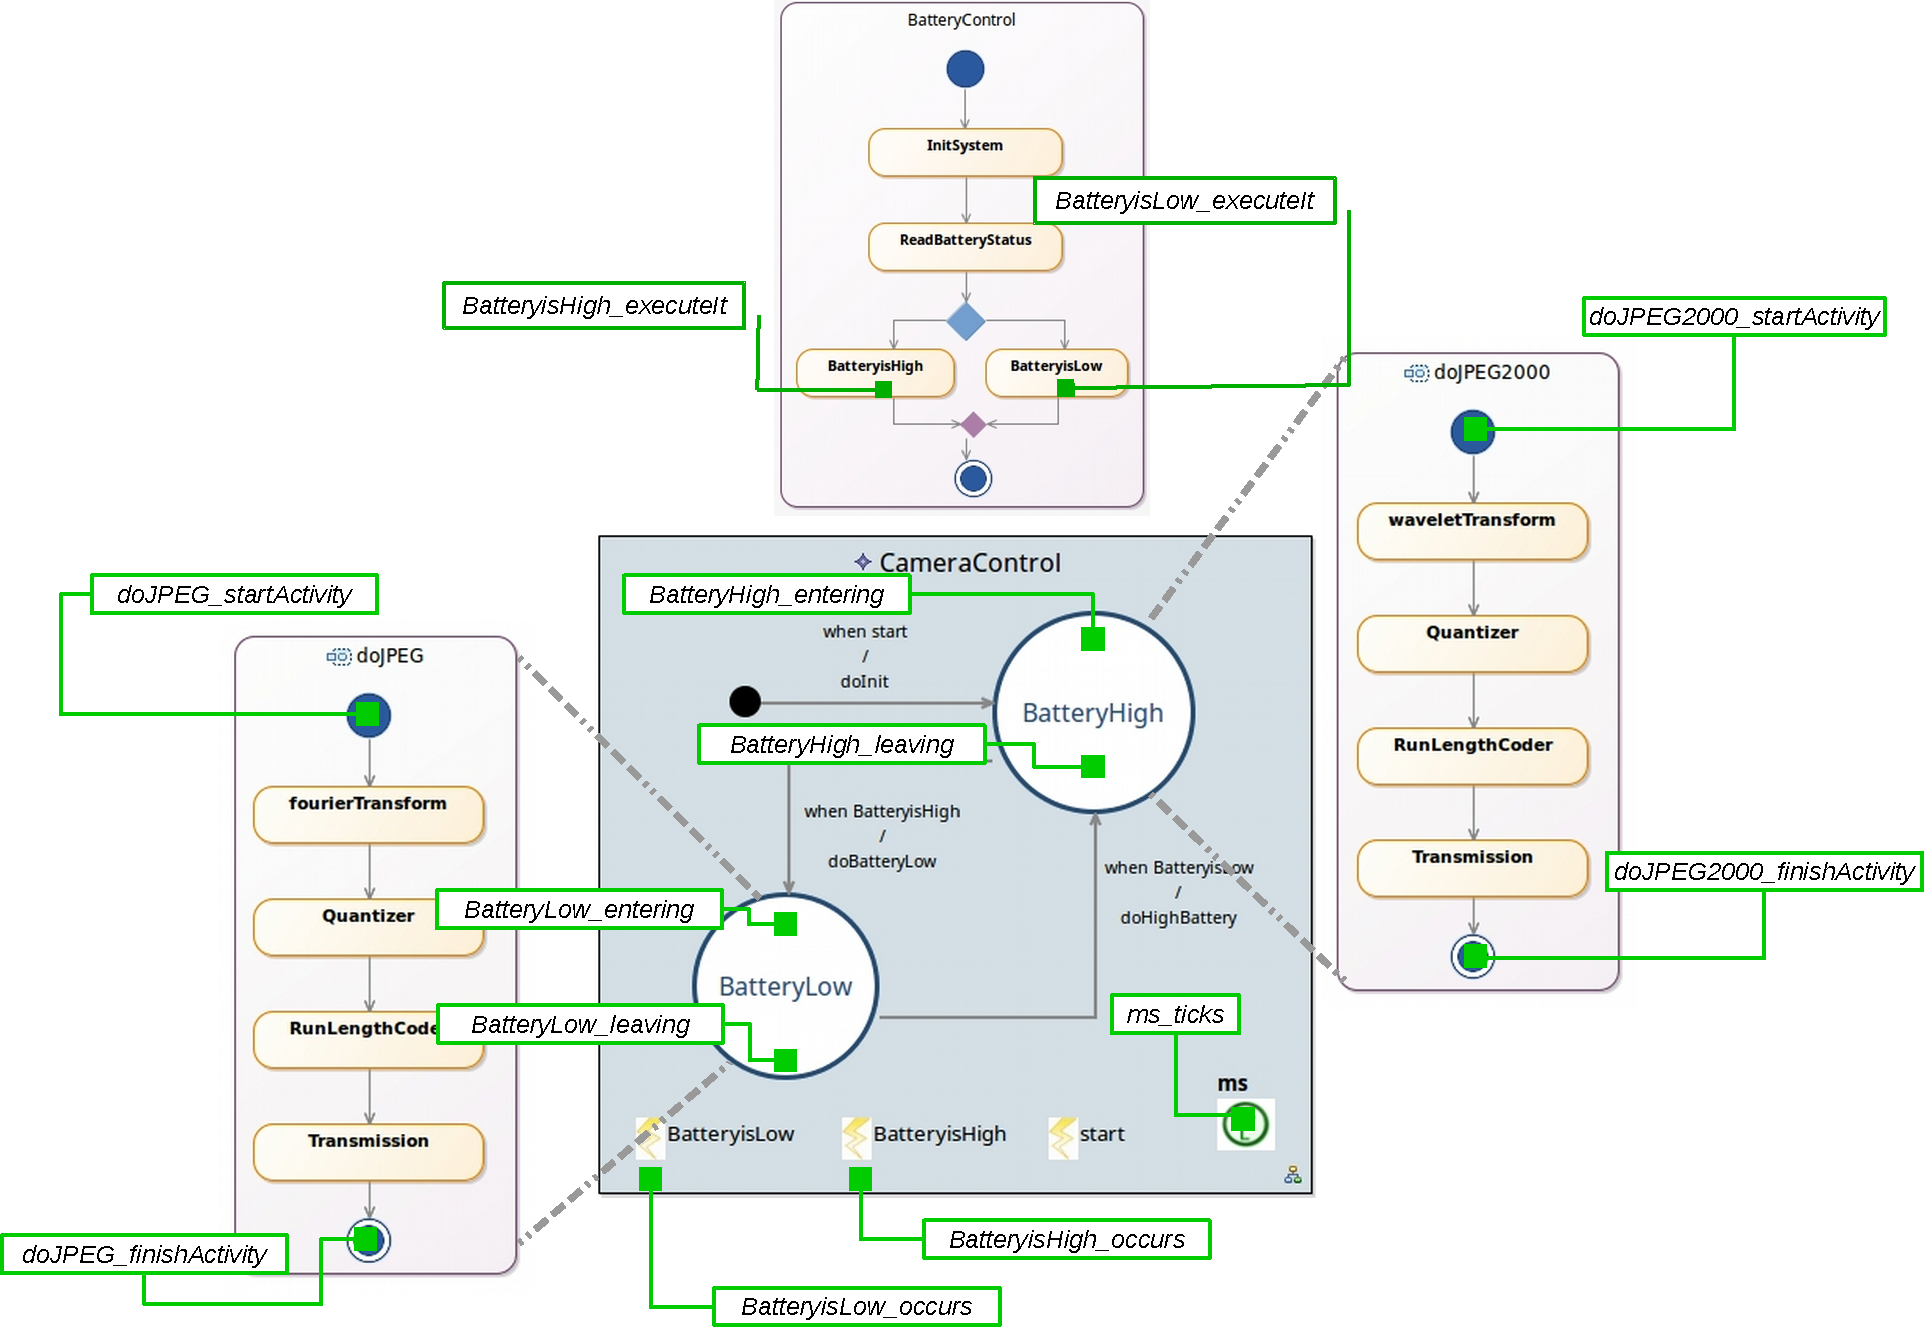
\includegraphics[width=.6\columnwidth]{examples/figs/picmodels.pdf}
		\caption{Hierarchical model of a surveillance camera system and a partial representation of the behavioral interface}
		\label{fig:camerasystem}
	\end{figure}
	
	To coordinate the models, we have to specify a timing and hierarchical coordination between the states of the TFSM CameraControl and the activities doJPEG and doJPEG2000. In addition, we have to synchronize the activity BatteryControl and the TFSM CameraControl by coordinating the corresponding Action and FSMEvent. Applying the four operators on these simple models, we generate the expected coordination specification. The coordination generated by using our approach corresponds to eight \ccsl relations.
	 
	In \bcool, the generated coordination specification conforms to the CCSL language. Since we are using a formal language, the integrator can execute and verify the coordination specification of the system.
	
	By using the language workbench presented in Section~\ref{section:bcoollengbench}, the coordination specification generated for the surveillance camera system can be executed and analysed. More precisely, we are able to execute the coordination specification by using TimeSquare, and to explore the state space. For lack of space we do not show the timing output of the execution of the surveillance camera system, however, the models together with a procedure to execute and verify them can be found in the companion web site.
	
	\todo{to show a timing and state space exploration}
	\subsection{Discussion}
	
	\begin{itemize}
		\item Discussion by relying on the criteria presented in evaluation.
		\item Semantics variation of the hierarchical coordination. 
		\item automatic generation of the coordination, eight relation.
		\item Verification and validation. 
	\end{itemize}

\section{Discussion}
	
\section{Conclusion}



% body of thesis comes here

\chapter{Conclusion}
\label{ch:conclusions}
In this thesis, we have proposed \bcool, a dedicated language that enables language integrators to specify coordination patterns between heterogeneous languages. By relying on this specification at language level, system designers can automatically generate the coordination between heterogeneous models. Such a model of coordination can be used to verify and execute the coordinated system. In the following, we summarize the main findings of this thesis. We finish this chapter by proposing future works. 

\section{Overview}
	
	
This thesis has focused on the coordination of heterogeneous behavioral models to provide execution and verification of the global system behavior. 

In the background section, we studied approaches that aim at getting the global representation of a heterogeneous system, in both structural and behavioral way. 

We first studied approaches that proposed to compose model/languages into a new model/languages. 

We have determined that theses approaches only focus on the syntactic of models. Only a few considers the behavior of models. However, they only compose homogeneous models thus limiting its in use in heterogeneous systems.     

Then, we presented approaches that proposed to coordination the behavior of heterogeneous models. 

They proposed to explicitly specify the interaction between behavioral models by using a dedicated language, \ie Coordination Languages and ADLs. 

We have noted that, in some of these approaches, the coordination is expressed in a formal language thus providing reasoning about the coordinated system. 


We have note that, to ease the task of a system designer, ADLs' community has successfully identified the need of connector types. Thus, a system designer has only to instantiate and bind connector types as needed by its architecture.

However, we have determined that the major drawback of coordination languages and ADLs is that the coordination is specified between particular models. With the increasing number and heterogeneity of the components, this task can quickly become difficult and error prone.

Then, we have presented four approaches that have identified that the instantiation and binding of connector types can be a systematic activity the system designer repeats many times and may consequently be defined as a coordination pattern. Such a pattern is based on the \emph{know-how} of the system designer and sometimes on naming or organizational conventions adopted by the models. These approaches have captured the specification of a behavioral coordination pattern inside a tool/framework to automate the instantiation and binding of connector types. These approaches go one step beyond Coordination Languages and ADLs by leveraging on the know-how of a system designer.

However, we have noted that, in these approaches, the knowledge about the coordination is hidden inside a tool, thus limiting reasoning. Moreover, they express the coordination in a GPL thus limiting the verification and validation of the coordinated system. Based on the state-of-art approaches, we have determined that:

\begin{itemize}
\item The specification of coordination patterns is specified at language level;
	 
\item The specification of coordination patterns should be done by using a dedicated language; 
	 
\item The coordination between models should be generated in a formal language to enable system designers to verify and validate the coordinated system. 		
\end{itemize}

We have determined that only four approaches have achieved to capture the specification of coordination patterns. We have determined that the lack of a systematic way to specify a coordination pattern makes these approaches ad-hoc and not flexible. Furthermore, this prevents a wider adoption of this sort of approaches. To understand how current approaches have achieved to capture a given coordination pattern, we have proposed a framework for the specification of coordination patterns. We have determined three building-blocks:

	\begin{itemize}
	\item A Language Behavioral Interface, which exposes partial information about the syntax and the behavioral semantics of languages for coordination purpose; 
	
	\item A Correspondence Rule, which specifies what and when elements from different languages must be coordinated;
	
	\item A Coordination Rule, which specify how the selected elements must be coordinated. 
\end{itemize}

We have used this frameowork to compare existing approaches. Then, we stated the requirements to make them more flexible and better customizable. More precisely, we proposed the requirements for a language to specified coordination patterns which supports heterogeneous languages and in which the coordination patterns can be customized. Based on these requirements, we proposed \bcool, a dedicated language to capture coordination patterns between languages. In our approach, we have proposed a language behavioral interface made of event types, \ie \dse. These event types act as coordination points on the language behavioral semantics. Then, we have proposed to specify coordination patterns by using operators that define a correspondence matching that selects instances of \dse, and a coordination rule that defines how the selected instances of \dse must be coordinated. Using \bcool, the know-how of a system designer is made explicit, stored and shared in libraries. Furthermore, such coordination patterns, expressed at the language level, can be applied on particular models to automatically generate the corresponding coordination model in \ccsl language. The use of the formal \ccsl language to express the coordination allowed us to provide execution and verification of the coordinated system.
	
We implemented \bcool as a set of Eclipse plugins integrated into the GEMOC studio. The studio proposed a language workbench and a modeling workbench. In the language workbench, an integrator can develop operators between languages. Then, in the modeling workbench, a system designer can use these operators to automate the coordination of models. We have proposed a dedicated language named \bflow that allows a system designer to specify what operators are applied on a set of models. Then, from this specification, a system designer can generate a model of coordination in \ccsl so that the whole system can be executed and verified.  
	
To validate our approach, we have presented the coordination of the heterogeneous models of a surveillance camera system. We modeled the different parts of the system by using the TFSM and Activity languages. To coordinate these models, we specified in \bcool three coordination patterns that we captured by using three operators. Unlike coordination frameworks in which the semantics of the coordination is hidden, we have explicitly specified these patterns by using a dedicated language. We used this specification to generate the coordination for the surveillance camera system, and then we executed the overall system.

	  
\section{Future Works}
\bcool provides some perspectives to extend and to improve the work carried out in this thesis. We list the propositions we consider essential to the continuity of this work:

\begin{itemize}
	\item \textbf{Extending \bcool to support the coordination of data:} System designers build coordination models to specify how models interact. The interactions between models can rely on events but also on data, \ie data-driven coordination. In this case, a model exchanges data with another model. With \bcool, we have managed interactions that rely on events, \ie control-driven coordination. To support the specification of coordination patterns that involve the exchange of data between models, we have to extend \bcool to support data driven coordination. More precisely, we have to add a way to specify when a value of a variable in a model is carried to a new value in a variable in another model. 
	%This makes arrive several questions:
	%		\begin{itemize}
	%			\item \emph{What} value must be carry, \eg the first one, the last one;
	%			\item \emph{When} the value of two variables must be synchronized, \eg immediately after one of them changes, after a period;
	%			\item \emph{How} the value of a variable must be carry from one model to another, \eg the same value, with some conversion. 
	%		\end{itemize}
	In \bcool, such information should be encoded in a \emph{data coordination rule}. In addition, the current coordination rule should be used to synchronize the events associated with the change of the value of a variable. Thus, the resulting model of coordination would have some \ccsl specification but also some code that represents the exchange of data between models. During the execution of models, such an exchange of data could be handled by the heterogeneous engine. Thus, a configuration file should be also generated to tell the engine what and when data from different models must be exchanged.	
	   	 
	\item \textbf{Generalizing the specification of correspondences by using a dedicated language:} In \bcool, the correspondence matching can capture implicit and explicit correspondences between elements of models. Currently, the explicit correspondence is only supported if one of the metamodel is modified to refer concepts from a different metamodel. To avoid such modification, we need a language to specify correspondences between concepts from different languages without modifying the metamodels (\eg like in megamodels~\cite{bezivinmegamodels}). This is, for instance, the case of Atlas Model Weaver~\cite{amwbib}, a tool that enables to create links between model elements. In~\cite{amwcompobib}, such links are used for model composition. Once links between models are established, a model transformation written in ATL can compose the model elements into a composed model. In our case, these links could be used to identified the elements to be coordinated. This is interesting, for instance, in the case of allocation in which there is a model of the hardware, a model of the application and a mapping model that is often generated by using some heuristic. Thus, the mapping model could be the input for a \bcool specification to generate the coordination model that represents the deployment between the hardware model and the platform model.
	%\item \textbf{Extending \bcool to generate a model of coordination in other language:} \bcool relies on \ccsl to express the coordination. However, we could rely on other coordination language to take advantages of the tooling from other environment. To do so, we have to investigate if the current event relations can be translated to another coordination language.\todo{bof...}
	
	\item \textbf{Using \bcool for the synthesis of the orchestrator for Co-Simulation of Functional Mock-up Units:} The analysis of Cyber-Physical Systems (CPS) involves the use of physical components (for instance described by differential equations evaluated according to the continuous time simulation paradigm) but it also involves the use of cyber components (usually relying on discrete time or discrete event simulation paradigms). Each language comes with existing tooling and several simulation tools and techniques are needed for CPS simulation and analysis. In this context, the Functional Mock-up Interface (FMI)~\cite{fmibib2} is a tool independent standard to support the co-simulation of dynamic models. The FMI standard provides a well defined specification and API to integrate heterogeneous simulation components. One key requirement for Co-Simulation via FMI is to develop a Master Algorithm that orchestrates the steps of Co-Simulation~\cite{fmibib}. For instance, the master algorithm has to control the data exchange and the time advancement among individual simulations. The FMI standard, however, does not describe or limit the implementation of the master algorithms. Currently, it is specified each time a particular system has to be co-simulated, which remains tedious and error prone. An interesting future work would be to generate such algorithm from a \bcool specification and the particular model used. Currently, the control and timing coordination is well managed by \bcool. However, to exploit the data exchange proposed by the FMI standard, it is mandatory to first extend \bcool to support data-driven coordination. 
	
	\item \textbf{Generalizing the specification of coordination patterns between existing modeling languages:} The development of heterogeneous system is currently done by using different existing modeling languages like Matlab, SDL or Modelica, which are developed by using very different technologies. To specify coordination patterns between these languages, we have to investigate how to add support for existing modeling languages in \bcool. Currently, to capture the specification of coordination patterns, we rely on partial information about the syntax and the behavioral semantics of languages that is contained in the language behavioral interface. It is thus mandatory that current modeling languages expose part of its syntax and behavioral semantics. The language behavioral interface may be a standard way to do it. In other words, modeling languages could provide a language behavioral interface for coordination purpose.    
				
		%\item It is thus mandatory a standard language behavioral interface. Such a language behavioral interface may be generated from code.   
	

	
	

	

	
		
				%\item To analyze CPS, some components can be easily described by differential equations, while others like communication networks require Discrete-Event Simulation (DEVS) techniques. As a result, several simulation tools and techniques are needed for CPS simulation and analysis. In particular, Co-Simulation (Cooperative Simulation) enables system designers to simulate individual components using different simulation tools.   
				
				%\item Cyber-Physical Systems (CPS) are composed of several collaborating physical and computing components that interact through embedded communication capabilities. 
		
		
		
		%\item Theoretically, an MA for direct co-ordination among FMUs can be developed for each distributed simulation problem, but that would be expensive and subject to errors.
		
\end{itemize}

%\appendix
% appendices come here
%\chapter{The TFSM and Activity Languages}
\label{ap:languages}
To illustrate the approach, we introduce a simple state-based language named Timed Finite State Machine (TFSM) and its behavioral interface; a state machine language augmented with timed transitions (see Figure~\ref{fig:tfsmmm}). The metamodel describes the abstract syntax of the TFSM language (see Figure~\ref{fig:tfsmmm}). A \emph{System} is composed of \emph{TFSMs}, global \emph{FSMEvents} and global \emph{FSMClocks}. Each \emph{TFSM} is composed of \emph{States}. Each state can be the source of outgoing guarded \emph{Transitions}. A guard can be specified either by the reception of an \emph{FSMEvent} (\emph{EventGuard}) or by a duration relative to the entry time in the source state of the transition (\emph{TemporalGuard}). When fired, transitions generate a set of simultaneous \emph{FSMEvent} occurrences.

The TFSM language defines the following \dse: \emph{entering} and \emph{leaving} a state, \emph{firing} a transition, the occurrences (\emph{occurs}) of a FSMEvent and the \emph{ticks} of a FSMClock (see at the top of Figure~\ref{fig:tfsmmm}). These \dse are part of the language behavioral interface of TFSM. \dse are defined by using a specific language named \ecl (standing for Event Constraint Language~\cite{ECL}) which is an extension of OCL~\cite{omgocl2} with events. \ecl takes benefits from the OCL query language and its possibility to augment an abstract syntax with additional attributes (without any side effects). Consequently by using \ecl, it is possible to augment \as metaclasses and add \dse. A partial \ecl specification of TFSM is shown in Listing~\ref{fig:tfsmmmecl} where the \dse \textit{entering} and \textit{leaving} are defined in the context of State (Listing~\ref{fig:tfsmmmecl}: line 6) while \textit{occurs} is defined in the context of FSMEvent (Listing~\ref{fig:tfsmmmecl}: line 4). When a metaclass is instantiated, the corresponding \dse are instantiated; \eg for each instance of the metaclass \emph{State}, \dse \textit{entering} is instantiated. Each instance of \dse is a \mse. In the case of TFSM, since two States are instantiated (\emph{S1} and \emph{S2}), there are two \mse of \textit{entering}: \textit{S1\_entering} and \textit{S2\_entering}. All \mse are part of the model behavioral interface. 
%\eject
\begin{figure}
	\begin{center}
		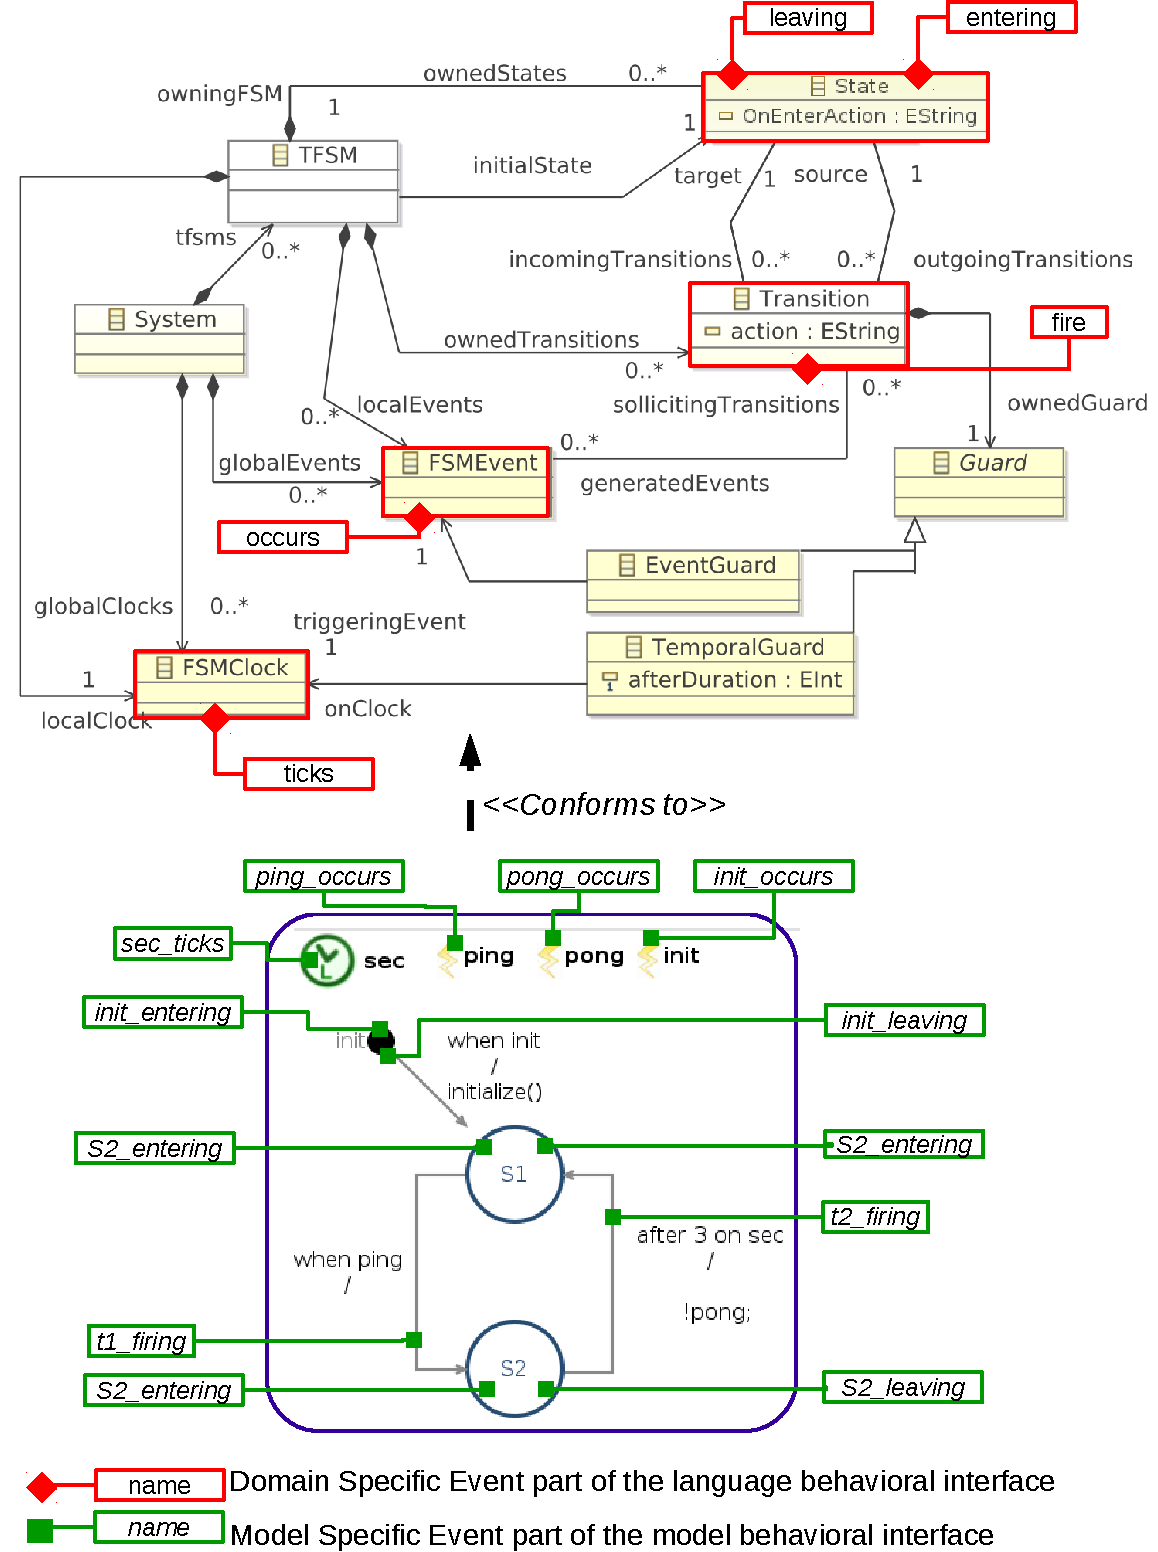
\includegraphics[width=1\textwidth]{bcool/figs/tfsmlang}
		\caption{(At the top) The TFSM metamodel with its language behavioral interface. (At the bottom)  a TFSM model with its model behavioral interface}
		\vspace{-2ex}
		\label{fig:tfsmmm}
	\end{center}
\end{figure}

\begin{lstlisting}[language=ecl,
caption={Partial \ecl specification of TFSM},
label={fig:tfsmmmecl}, 
basicstyle=\scriptsize\ttfamily, backgroundcolor=\color{LGrey}, numbers=left, xleftmargin=3pt]
package tfsm
context FSMClock
def: ticks : Event = self
context FSMEvent
def: occurs : Event = self
context State
def : entering : Event = self
def : leaving : Event = self
\end{lstlisting}

\todo{Interface of Activity}


Before going into the example, we briefly present the language behavioral interface of the fUML language partially shown in  Listing~\ref{fig:eclfuml}. For each \emph{Activity} two \dse are defined: \emph{startActivity} and \emph{finishActivity}, to identify respectively the starting and finishing instants of the activity. Similarly, Two \dse are defined for each \emph{Action}: \emph{startAction} and \emph{finishAction}, to identify the starting and the finishing of an Action. These \dse, part of the fUML language behavioral interface, are used throughout this section to specify the coordination operators.

\begin{lstlisting}[language=ecl,
caption={Partial \ecl specification of Activity Diagram},
label={fig:eclfuml}, 
basicstyle=\scriptsize\ttfamily, backgroundcolor=\color{LGrey}, numbers=left, xleftmargin=3pt, belowskip=-0.4em]
package uml
context Activity
def: startActivity : Event = self
def: finishActivity: Event = self
context Action
def : startAction : Event = self
def : finishAction : Event = self
\end{lstlisting}

%\chapter{Event Expression and Event Relations}
\label{ap:expressionandrelations}

\todo{To add Filter()}

\todo{To add Sample()}


\todo{To add Rendezvous()}


		
		\begin{figure}
			\center
			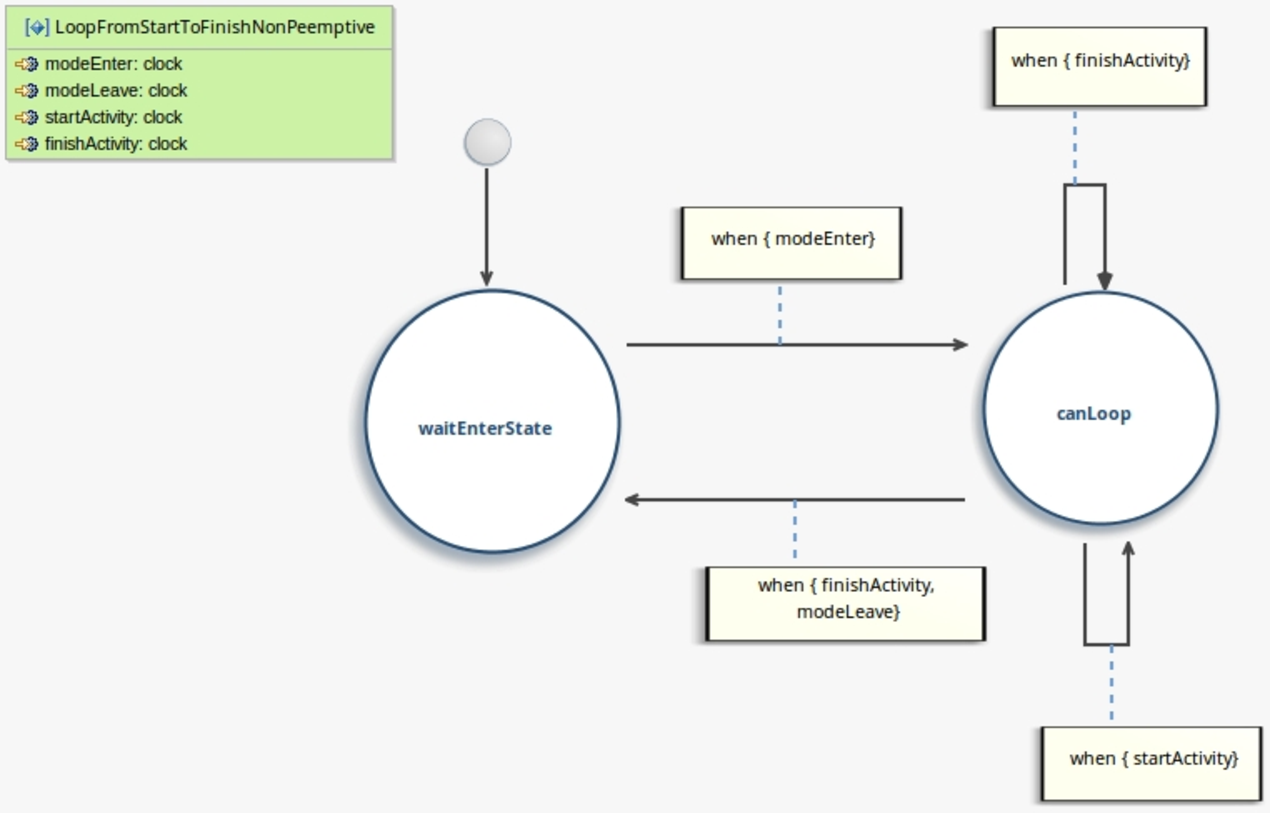
\includegraphics[scale=0.5]{examples/figs/LoopFromStartToFinishNonPreemptive}
			\caption{Graphical Representation of the Event Relation \emph{LoopFromStartToFinishNonPreemptive}}
			\label{fig:LoopFromStartToFinishNonPreemptive}
		\end{figure}



		\begin{figure}
			\center
			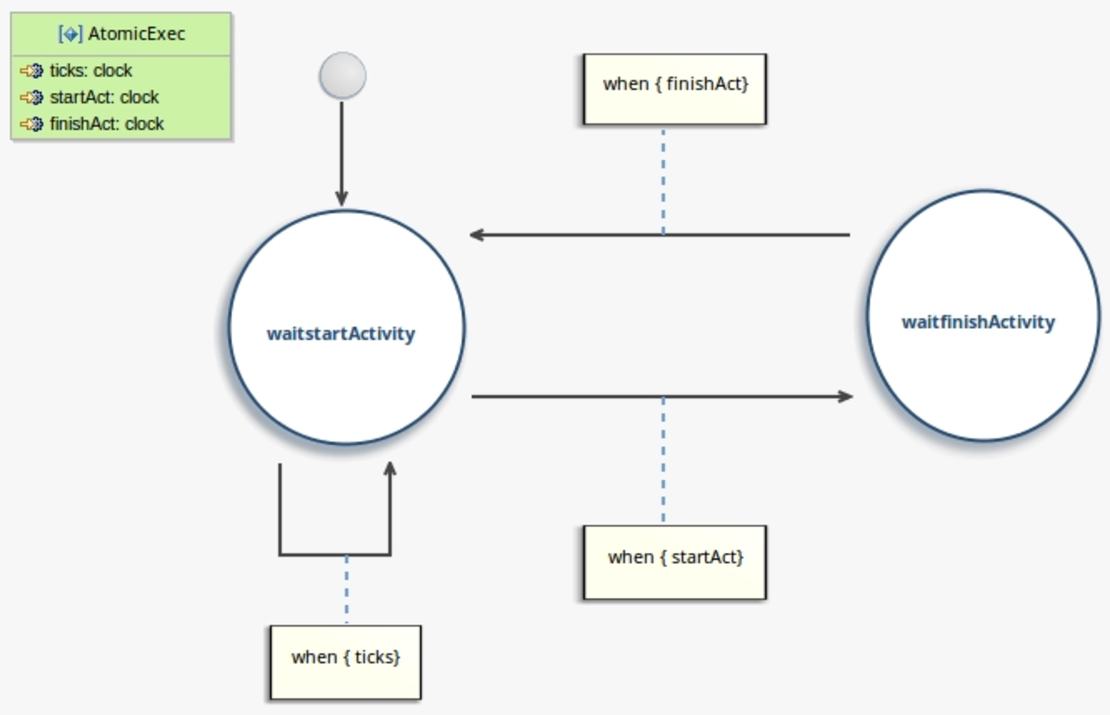
\includegraphics[scale=0.5]{examples/figs/AtomicExec}
			\caption{Graphical Representation of the Event Relation AtomicExec}
			\label{fig:AtomicExec}
		\end{figure}
		


\addcontentsline{toc}{chapter}{Bibliography}
\bibliographystyle{alpha}
\bibliography{bibliography/bibliography}

\end{document}